% !TEX encoding = ISO-8859-16
%%%%%%%%%%%%%%%%%%%%%%%%%%%%%%%%%%%%%%%%%%%%%%%%%%%%%%%%%%%%%%%%
%%%%%%%%%%%%%%%%%%%%%%%%%%%%%%%%%%%%%%%%%%%%%%%%%%%%%%%%%%%%%%%%
\section{Numerical Illustrations}
\label{sec:results}

We emphasize that this paper introduces two different approaches (Sliced and Radon) together with their corresponding discretization (Lagrangian and Eulerian) to cope with the variety of image processing and computer graphics applications that optimal transport is targeting. This section compares these two methods on synthetic examples and explores a few of these applications in order to illustrate the relative benefit of each method. 


%%%%%%%%%%%%%%%%%%%%%%%%%%%%%%%%%%%%%%%%%%%%%%%%%%%%%%%%%%%%%%%%
\subsection{A Case Study: Sliced Wasserstein Distance for Pairs of Diracs}
\label{subsec-twodiracs}

As discussed in Section~\ref{subsec-sliced-assignement}, we empirically found that the sliced Wasserstein distance $X \mapsto \SWass{\RR^d}(\mu_X,\mu_Y)$ to a given measure $\mu_Y$ for $Y \in \RR^{N \times d}$ has no local minimum, i.e., only has global minima satisfying $\mu_X=\mu_Y$, saddle points, and local maxima. This is of primary importance because in practice a descent scheme avoids saddle points and local maxima (since these are unstable stationary point of the flow), and the gradient flow~\eqref{eq-flow-swass} converges to a global minimum, which in turn defines an assignment. 

While we do not give a formal proof of this statement, we illustrate this point on a simple example in 2-D (i.e. $d=2$) with point clouds having two masses (i.e. $N=2$). We fix 
\eq{
	\choice{
		Y = \{ Y_1, Y_2 \} = \{ (0,-1), (0,+1) \}
		\qandq\\
		{X(u) = \{ X_1, X_2 \} = \{ u, -u \}},
	}
} 
and only let $u=(x,y) \in \RR^2$ varies (see Figure~\ref{fig-comparison} for an illustration). We then compare the Wasserstein and Sliced Wasserstein distances
\eq{
	\foralls u \in \RR^2, \quad \choice{
	\Ee^{W}(u) = \Wass{\RR^2}( \mu_{X(u)}, \mu_Y )^2, \\ 
	% = 2\left(x^2 + (\lvert y\rvert-1)^2\right), \\
	\Ee^{S}(u) = \SWass{\RR^2}( \mu_{X(u)}, \mu_Y )^2, \\
	% = x^2+y^2 +1 - \frac{4}{\pi} \left( x + y atan(\frac{y}{x}\right), \\
	\Ee^{S}_\Theta(u) =\frac{1}{\lvert \Th \rvert} \sum_{\th \in \Th} \Wass{\RR}( P_\th \sharp \mu_{X(u)}, P_\th \sharp \mu_Y )^2.
	}
}
After some calculations, we get the following expressions for $\Ee^{W}$ and $\Ee^{S}$
\eq{
	\foralls (x,y) \in \RR^2, \; \choice{
	\Ee^{W}(x,y) = 2\left(x^2 + (\lvert y\rvert-1)^2\right), \\
	\Ee^{S}(x,y) = x^2+y^2 +1 - \frac{4}{\pi} \left( x + y \cdot \text{atan}\left(\frac{y}{x}\right)\right)
	}
}
while $\Ee^{S}_\Theta(u)$ is evaluated numerically using a discrete set of orientations $\Theta$.
Figure~\ref{fig-comparison} shows a comparison of these two distances. We can see that the Sliced Wasserstein distance (as well as the Wasserstein distance) has no local minimum, although there are three saddle points at $u=(0,0)$ and {$u=\pm(\frac{2}{\pi}, 0)$}, which separate two basins of attraction associated to the two global 
minima. 
% \cmt{Note that the approximate energy $\Ee^{S}_\Theta$, here evaluated using $\lvert \Th \rvert=10$ equi-spaced directions, has the same properties.}


\begin{figure*}[!tb]
\begin{center}
\begin{minipage}[p]{0.2\linewidth}
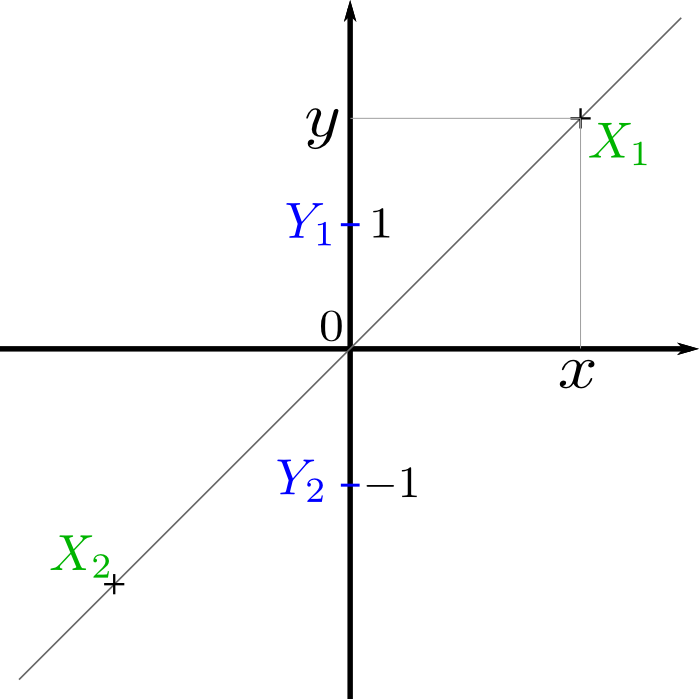
\includegraphics[width=\linewidth]{2diracs/Illustration_deux_points_symetrique_2D}
\end{minipage}
\hfill
\begin{minipage}[p]{0.79\linewidth}
\begin{tabular}{c@{}c@{}c@{}} % @{}c@{}
%\multirow{2}{*}{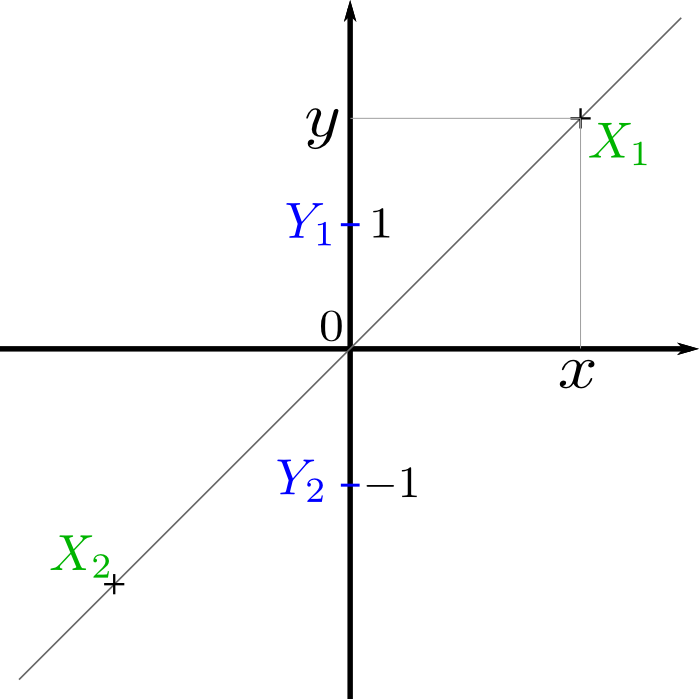
\includegraphics[width=0.24\linewidth]{2diracs/Illustration_deux_points_symetrique_2D}\vspace*{0.12\linewidth}} &
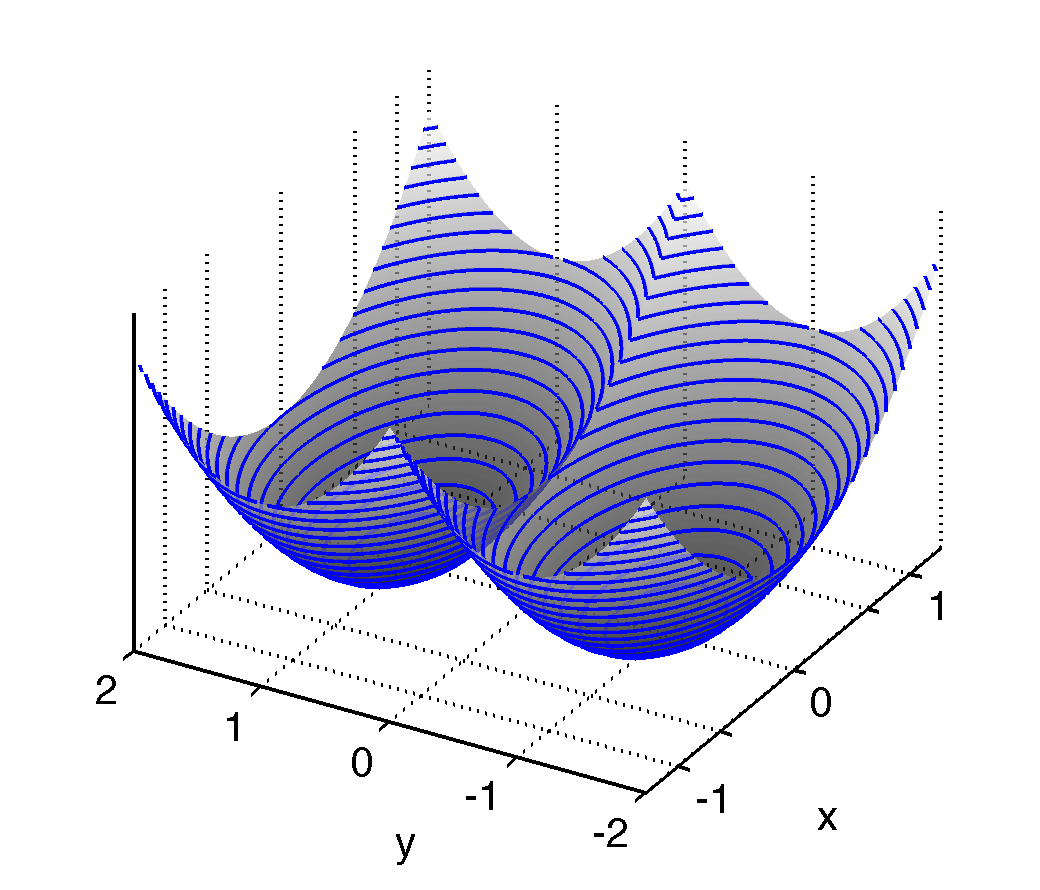
\includegraphics[width=0.33\linewidth]{2diracs/surf_W2_v3}&
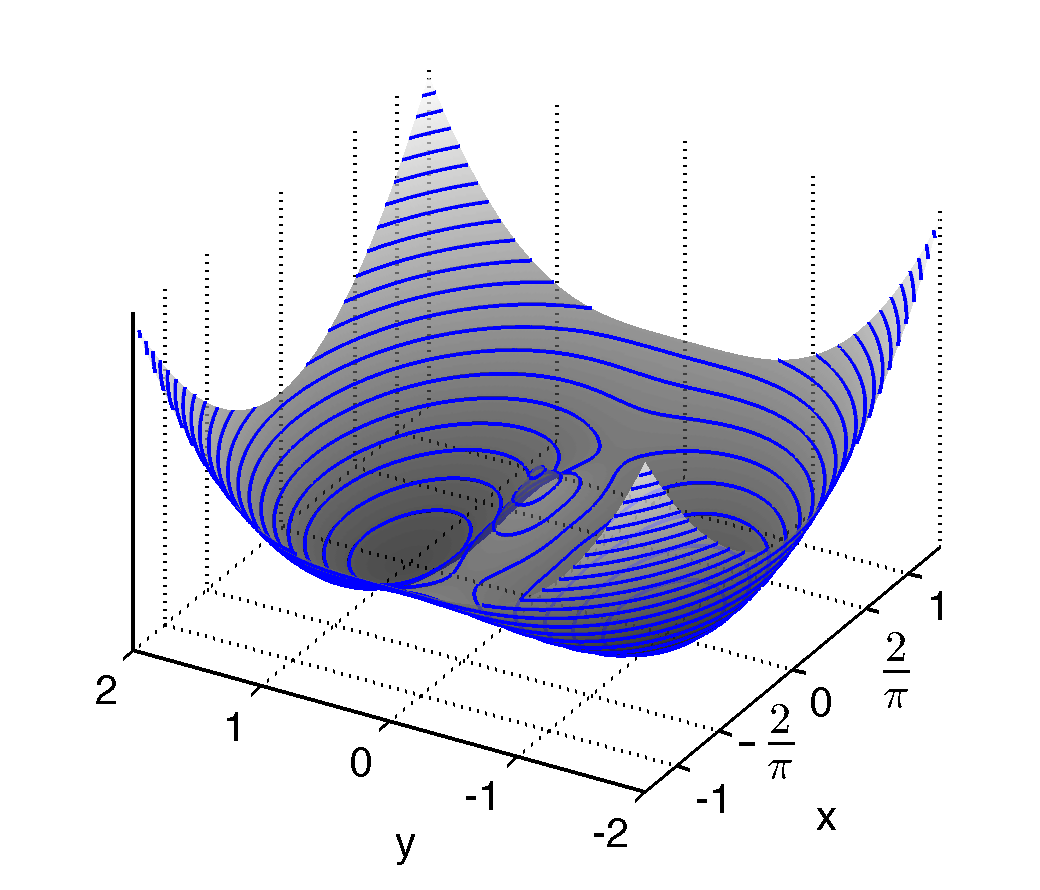
\includegraphics[width=0.33\linewidth]{2diracs/surf_SW2_v3}&
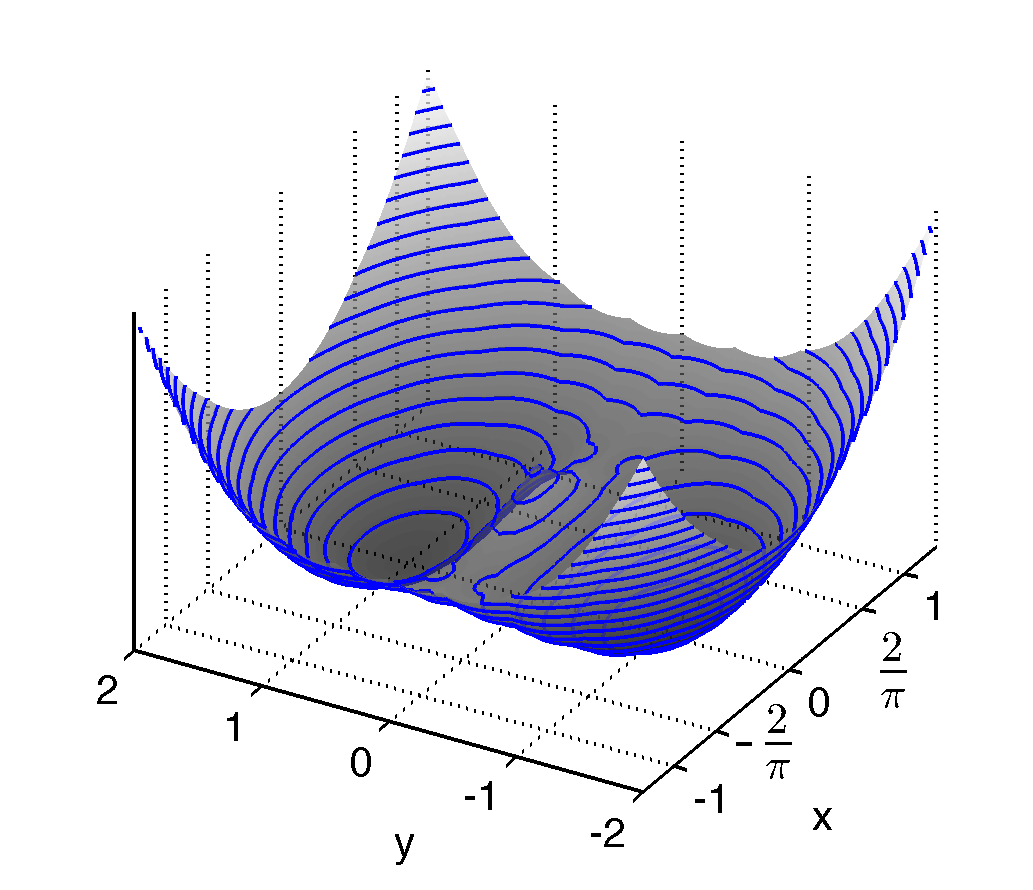
\includegraphics[width=0.33\linewidth]{2diracs/surf_SW2_10dir_v3}
\\
%&
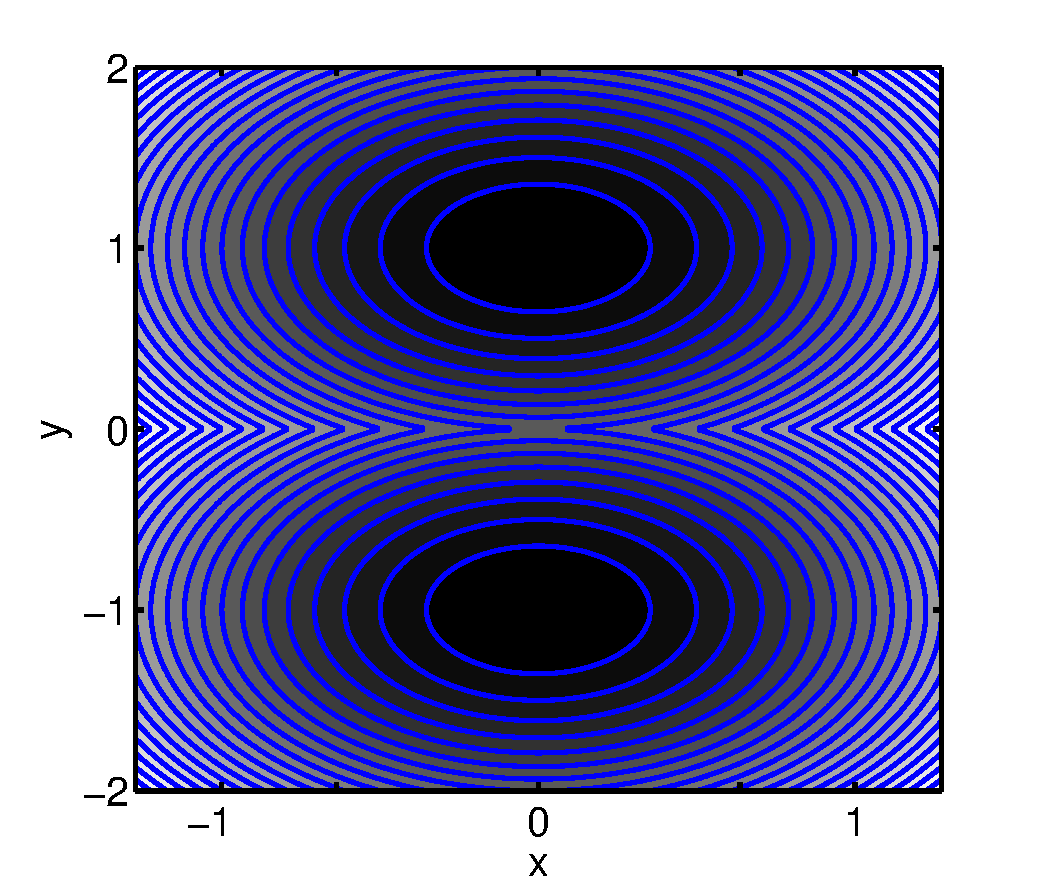
\includegraphics[width=0.33\linewidth]{2diracs/contour_W2_v3}&
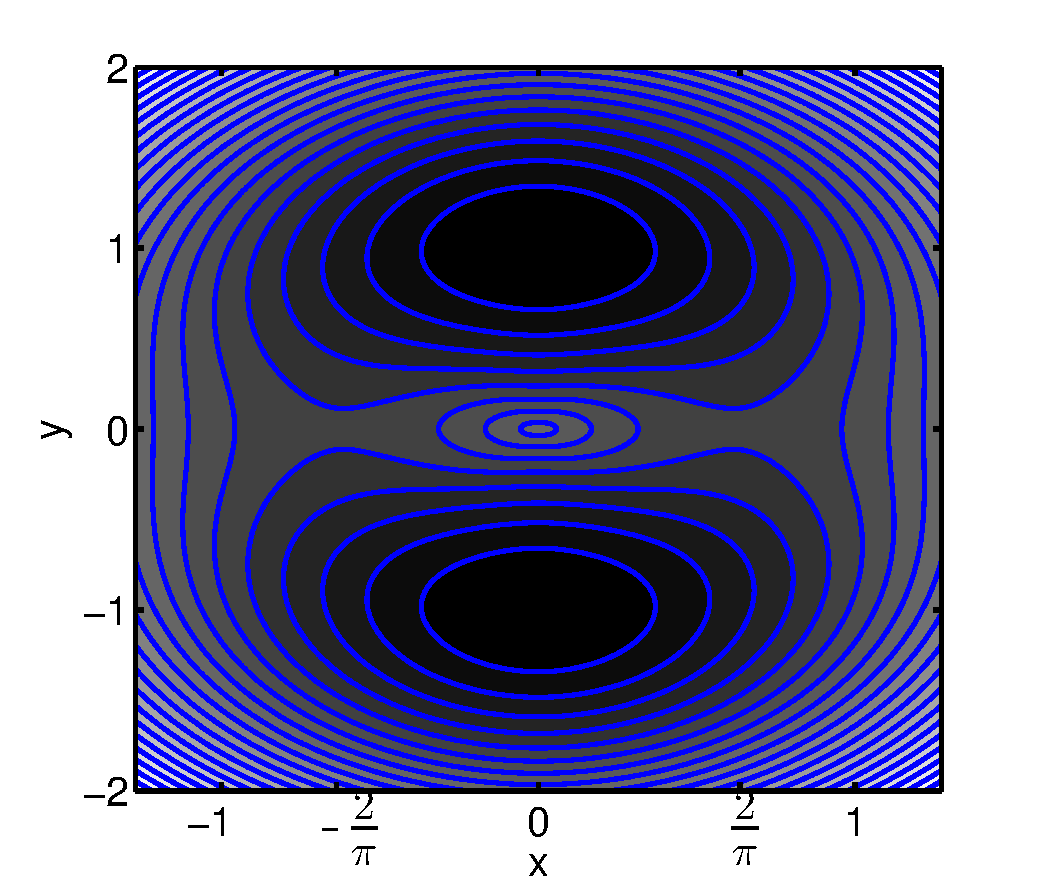
\includegraphics[width=0.33\linewidth]{2diracs/contour_SW2_v3}&
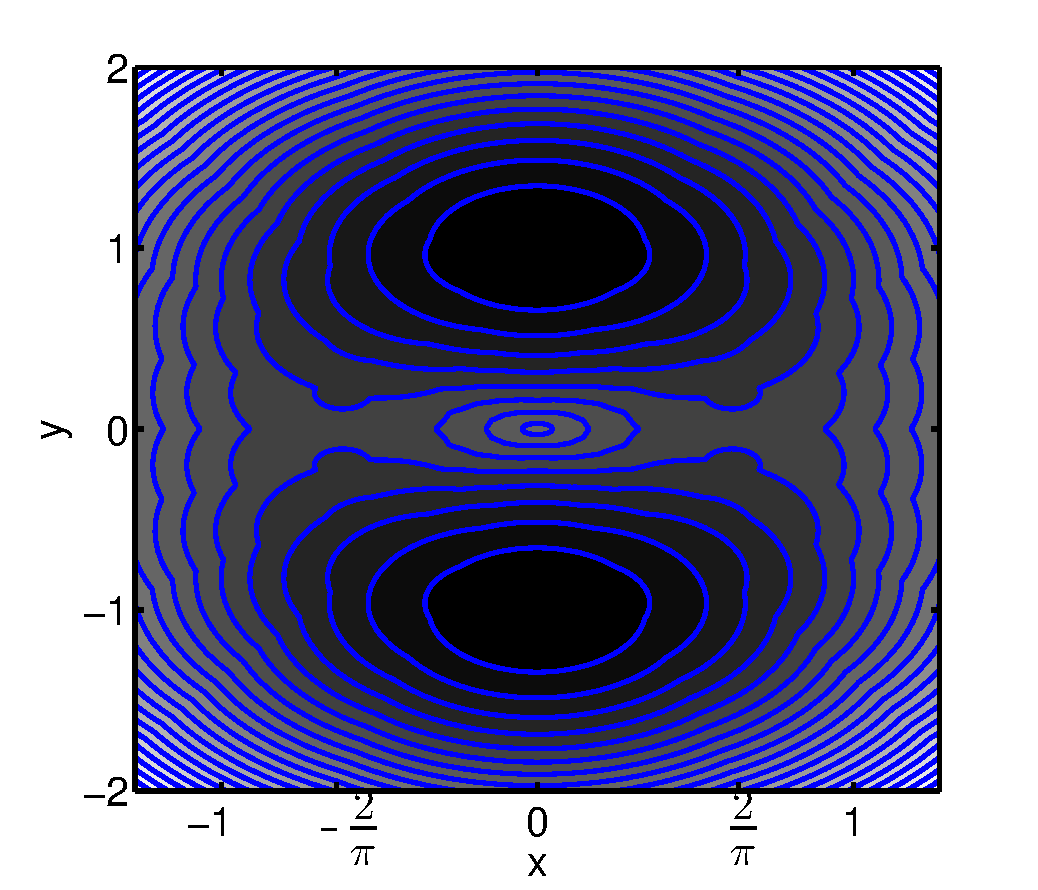
\includegraphics[width=0.33\linewidth]{2diracs/contour_SW2_10dir_v3}
\\
%&
$\Ee^{W}(x,y)$ & $\Ee^{S}(x,y)$ & $\Ee^{S}_\Theta(x,y)$ with $|\Theta|=10$.
\end{tabular}
\end{minipage}
\end{center}
\caption{Comparison of $\SWass{\RR^2}^2$ and $\SWass{\RR^2}^2$, and its numerical approximation using 10 directions, as an elevation surface (top row) and its corresponding 2d map (bottom row).}
\label{fig-comparison}
\end{figure*}



%%%%%%%%%%%%%%%%%%%%%%%%%%%%%%%%%%%%%%%%%%%%%%%%%%%%%%%%%%%%%%%%
\subsection{Numerical Considerations for the Sliced Transport}
\label{subsec-num-stochastic}


%%%%%
\newcommand{\mydisplay}[1]
{
%
\hline &\\
Ref. &
\begin{tabular}{c@{\hspace{6mm}}c@{\hspace{6mm}}c@{}}
\includegraphics[width=0.18\linewidth]{interp_stochastic/#1_mu_1}&
\includegraphics[width=0.18\linewidth]{interp_stochastic/#1_mu_W2bary}&
\includegraphics[width=0.18\linewidth]{interp_stochastic/#1_mu_2}
\\
 $\mu_0$ & $\mu^{W}_\frac{1}{2}$   & $\mu_1$
\end{tabular}
\\
$\mu^{S}_\frac{1}{2}$ &
\begin{tabular}{c@{\hspace{2mm}}c@{\hspace{2mm}}c@{\hspace{2mm}}c@{}}
\includegraphics[width=0.18\linewidth]{interp_stochastic/#1_mu_SW2interp_2dir}&
\includegraphics[width=0.18\linewidth]{interp_stochastic/#1_mu_SW2interp_20dir}&
\includegraphics[width=0.18\linewidth]{interp_stochastic/#1_mu_SW2interp_200dir}&
\includegraphics[width=0.18\linewidth]{interp_stochastic/#1_mu_SW2interp_2000dir}
\\
$\abs{\Th_\ell}=2$ &
$\abs{\Th_\ell}=20$ &
$\abs{\Th_\ell}=200$ &
$\abs{\Th_\ell}=2000$
\end{tabular} \\
%
}
%%%%%

\begin{figure}[!t]
\begin{center}
\begin{tabular}{|c|c|}
%
\mydisplay{48701}
\mydisplay{117925}
\mydisplay{799530}
%
\\
\hline
\end{tabular}
\end{center}
\caption{ %\textit{Influence of the $\Sph$ discretization for the Sliced Wasserstein transport.}
We consider the optimal Wasserstein barycenter $\mu^{W}_\frac{1}{2}$ between $\mu_0$ and $\mu_1$.
We show the Sliced Wasserstein interpolation $\mu^{S}_\frac{1}{2}$ using our stochastic Newton descent \eqref{eq-stoch-grad-desc} %\eqref{eq-grad-desc-sliced_newton}.
with different number of directions $\abs{\Th_\ell}$. The density is displayed using a Parzen density estimation.
}
\label{fig:interp_stochastic}
\end{figure}

\paragraph{Influence of the number of directions. } 

We first illustrate the special case discussed in Section~\ref{subsec-sliced-assignement} of the transport of a discrete distribution (a sum of Dirac masses) $\mu_0$ toward another, $\mu_1$. This boils down to an assignment problem. We resort to the stochastic gradient descent detailed in \eqref{eq-stoch-grad-desc} to compute a Sliced Wasserstein transport $T^S$.
This map $T^S$ always numerically verifies $T^S\#\mu_0 = \mu_1$. Nevertheless, it can be far from the optimal Wasserstein transport map $T^W$ when using a small number of directions at each iteration.
We illustrate this in Figure~\ref{fig:interp_stochastic}, that shows the distributions obtained when interpolating the transport map $T^S$, that is, we compute $\mu_{\lambda}^S = [(1-{\lambda}) \Id +  \lambda T^S] \sharp \mu_0$ for $\la \in [0,1]$, when varying the number of directions $\Th_\ell$ used at each iteration.
Using more sampling directions tends to provide more regular transport maps.  However, we note that the Sliced Wasserstein transport can provide a different assignment from the optimal Wasserstein map, even when using a large set of directions (Fig.~\ref{fig:interp_stochastic}, third example).

%%%
\paragraph{Influence of local minima.} 

Since the algorithm detailed in Section~\ref{subsec-algorithm-lagrangian} performs a non-convex energy minimization (see~\eqref{eq-non-convx-pointclouds}), it is important to understand the influence of the initialization of the descent. Figure~\ref{fig:rnd_init} analyzes on a simple example the effect of the presence of local minima. The center plots (b) and (c) each show two results (blue and red dots) approximating the sliced iso-barycenter $\mu^S_{1/2}$ %(middle point of the geodesic) \cmt{at this stage, we have already used it a lot, and the definition is obvious}
%\eq{
	%\mu_{1/2} = \Bary{\RR^d}^S \left( (\mu_0,\mu_1), (\tfrac{1}{2},\tfrac{1}{2}) \right).
%}
using our non-convex gradient descent, as well as the Wasserstein barycenter $\mu^W_{1/2}$ (black dots) computed via linear programming since there are only two distributions. 
Each result is obtained using a random initialization with samples independently drawn from an isotropic Gaussian having the same mean and variance as $\mu_0$. While this clearly shows that different initializations lead to different estimates, this also shows that the impact of the initialization is quite modest. 


\begin{figure*}[!t]
\begin{center} 
\begin{tabular}{@{}c@{\hspace{5mm}}c@{\hspace{5mm}}c@{\hspace{5mm}}c@{}}
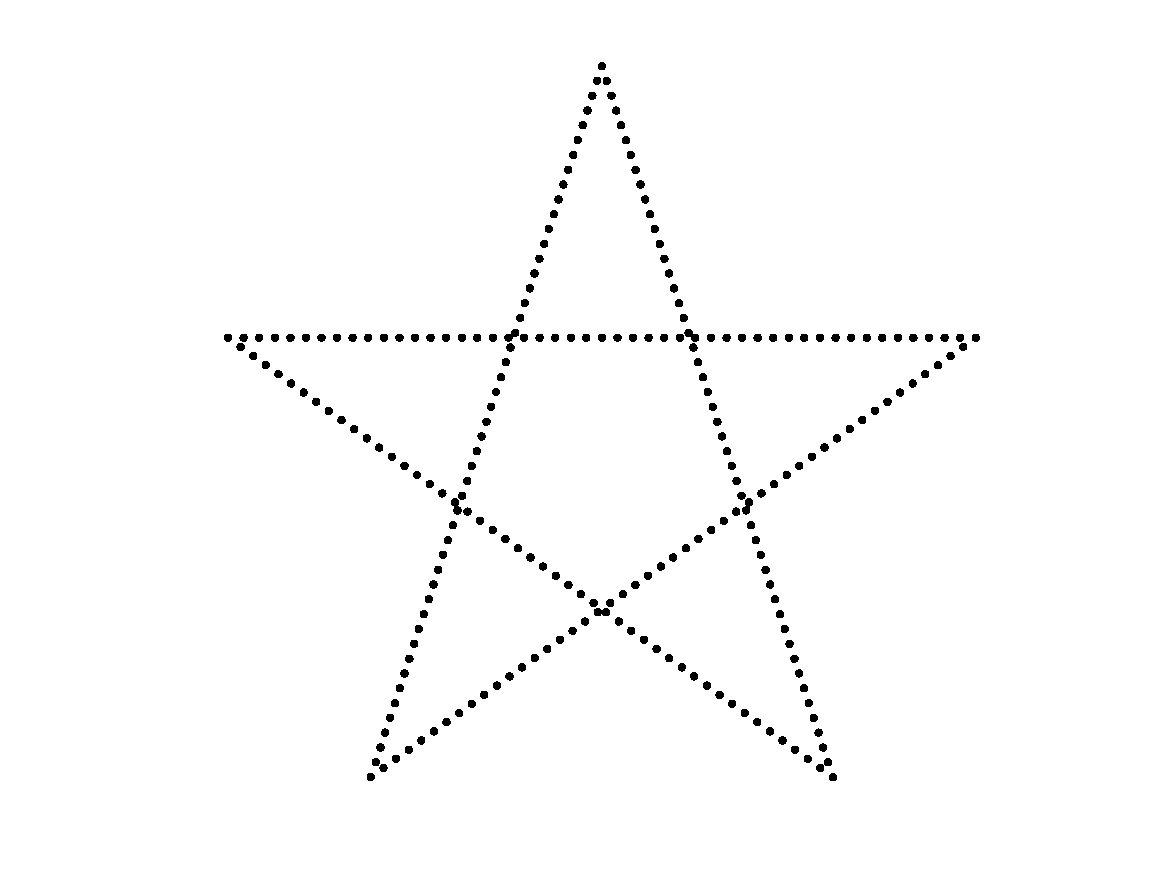
\includegraphics[width=0.23\linewidth]{init/star_v1}&
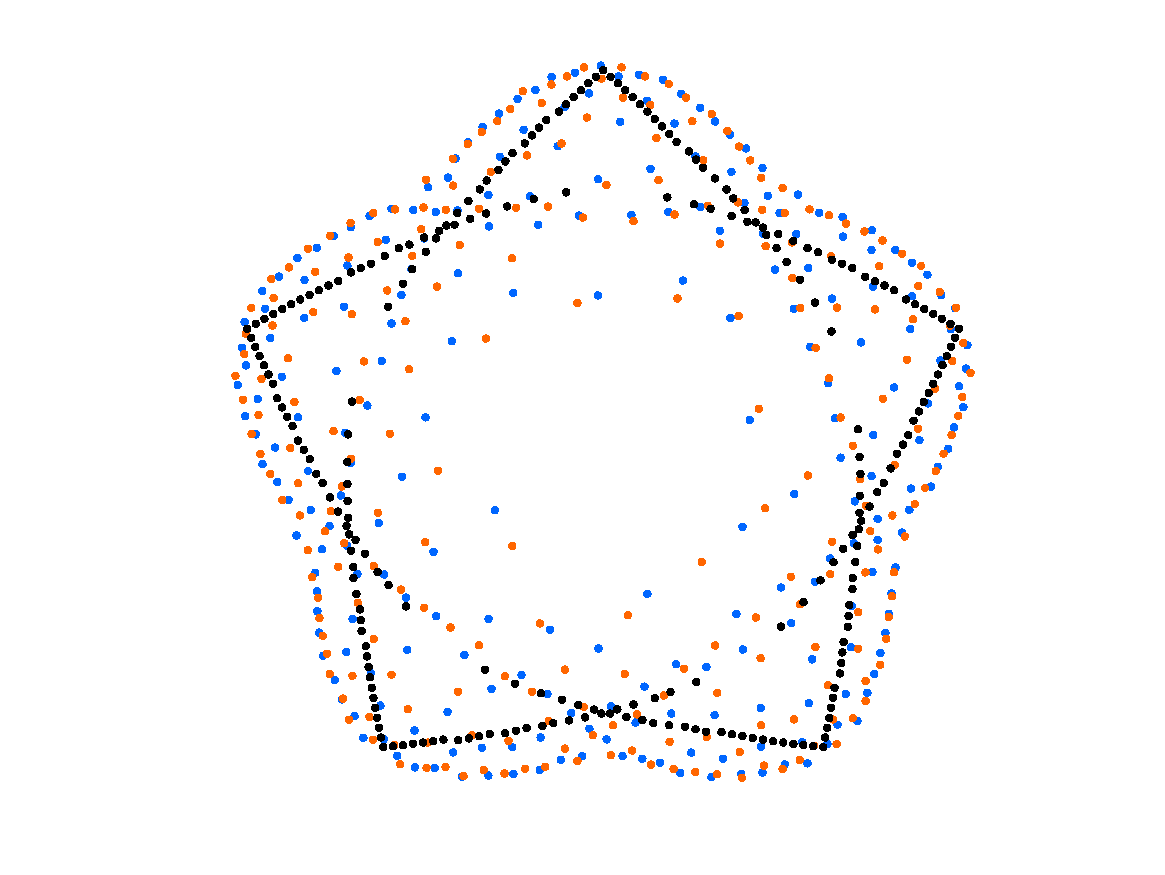
\includegraphics[width=0.22\linewidth]{init/circle_star_sw_bary_rnd_init_1000_v1}&
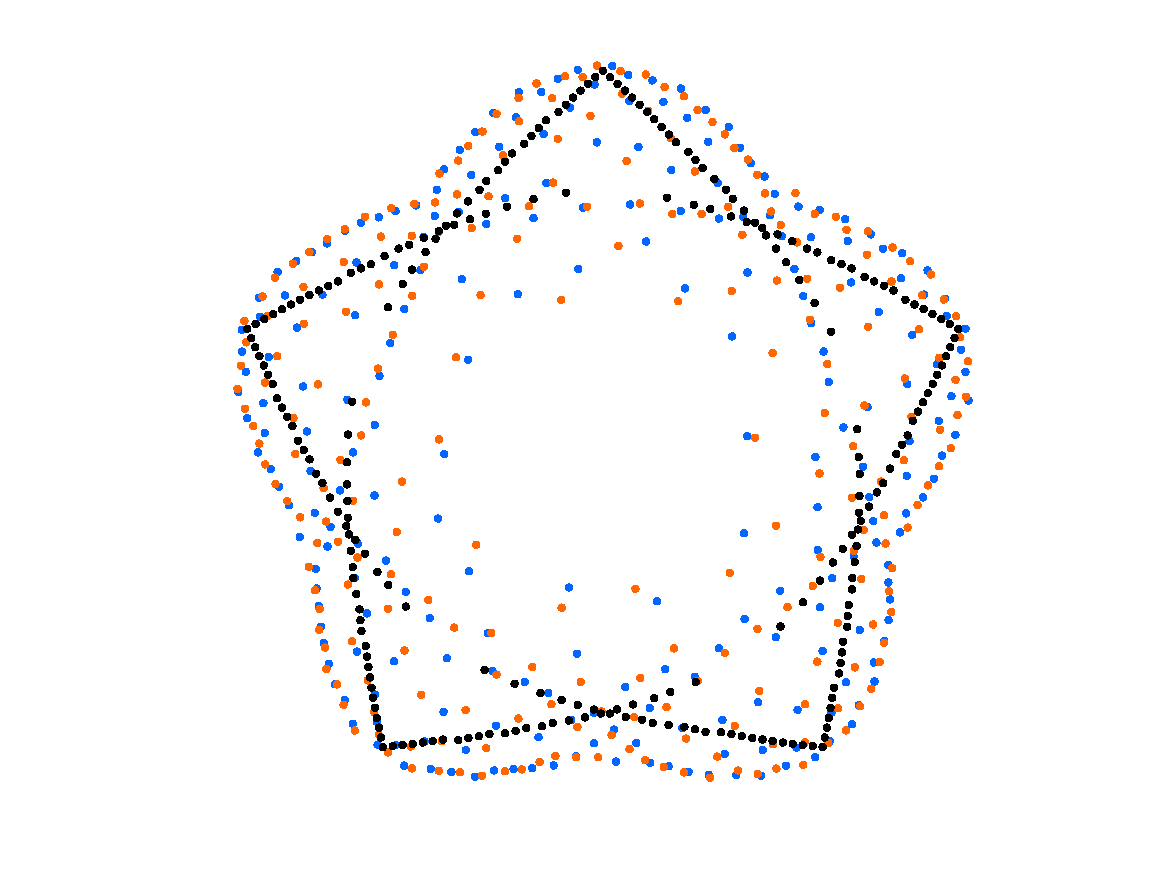
\includegraphics[width=0.22\linewidth]{init/circle_star_sw_bary_rnd_dir_1000_v1}&
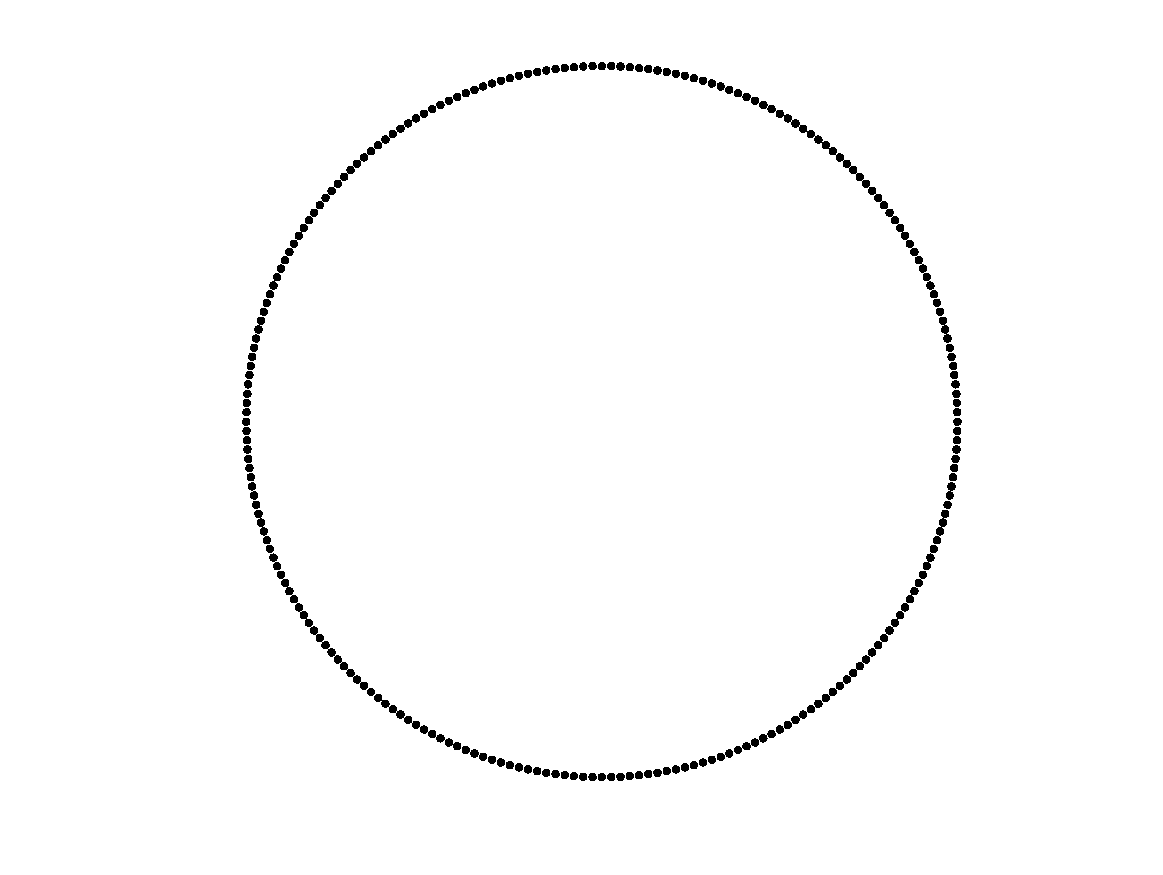
\includegraphics[width=0.22\linewidth]{init/circle_v1}\\
(a) $\mu_0$  & (b) $\mu^S_{1/2}$ (uniform $\Th$) & (c) $\mu^S_{1/2}$ (random $\Th$) & (d) $\mu_1$
\end{tabular}
\end{center}
\caption{ Influence of the initialization $X^{[0]}$ and the directions set $\Theta$ (here $\lvert\Theta\rvert=10^3$) on our Lagrangian discretization of the sliced barycenter. 
The black point cloud corresponds to the Wasserstein interpolation $\mu^W_{1/2}$ of the two distributions $\mu_0$ and $\mu_1$.  The red and blue point clouds correspond to the sliced Wasserstein barycenters obtained with different settings: (b) using two random point 
clouds initializations for $X^{[0]}$ with the same set of directions $\Theta$ (equi-spaced on the circle);  (c) using the same initializations $\mu_{X^{[0]}} = \mu_0$ but with different uniformly sampled random directions $\Theta$.}
\label{fig:rnd_init}
\end{figure*}



%%%%%%%%%%%%%%%%%%%%%%%%%%%%%%%%%%%%%%%%%%%%%%%%%%%%%%%%%%%%%%%%
\subsection{Numerical Comparison of the Barycenters}
\label{subsec-num-comparison}

This section compares the following barycenters in a 2-D ($d=2$) setting:
\begin{itemize}
	\item[--] The original Wasserstein barycenter $\Bary{\RR^d}^W$ (see Definition~\ref{defn-wass-baryc}), which can only be computed numerically for $2$ distributions, i.e. $|I|=2$, and thus corresponds to the Wasserstein geodesic between the two measures. We use the proximal splitting method of~\cite{FPapPeyOud13} to estimate this barycenter with a Eulerian discretization on a fixed grid.	%\todo{and which approach for the Lagrangian version? (in Fig.2) : I used Hungarian Algorithm for small point clouds and Mosek library for larger point clouds (simplex or interior point primal-dual methods)} 
	\item[--] The Radon barycenter $\Bary{\RR^d}^R$ (see Definition~\ref{defn-radon-baryc}). It is approximated with the numerical scheme presented in Section~\ref{subsec-algorithm-eulerian} with an Eulerian discretization. 
	\item[--] The sliced barycenter $\Bary{\RR^d}^S$ (see Definition~\ref{defn-sliced-baryc}). It is approximated with the numerical scheme presented in Section~\ref{subsec-algorithm-lagrangian} with a Lagrangian discretization. If not stated otherwise, we use $|\Theta|=10$ directions uniformly sampled on the half circle. 
\end{itemize}



%%%
\paragraph{Comparison of the Sliced, Radon and Wasserstein Geodesics.} 

In general, the sliced and Radon barycenters differ from the original Wasserstein barycenter. While the Wasserstein barycenter of Gaussian distributions is always a Gaussian distribution~\cite{Carlier_wasserstein_barycenter}, Figure~\ref{fig:aniso} shows that this is not the case for the Radon barycenter when the Gaussians are not isotropic.

\begin{figure}[!t]
\begin{center}
\begin{tabular}{@{}c@{}c@{}c@{}c@{}c@{}}

\includegraphics[width=0.19\linewidth]{gaussian-geod/anis0_padding}&
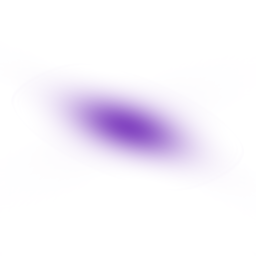
\includegraphics[width=0.19\linewidth]{gaussian-geod/anis1_padding}&

\includegraphics[width=0.19\linewidth]{gaussian-geod/anis2_padding}&

\includegraphics[width=0.19\linewidth]{gaussian-geod/anis3_padding}&

\includegraphics[width=0.19\linewidth]{gaussian-geod/anis4_padding}\\
$t=0$ & $t=1/4$ & $t=1/2$ & $t=3/4$ & $t=1$
\end{tabular}
\end{center}
\caption{ The Radon geodesic $\mu_t = \Bary{\RR^d}^R( (\mu_0,\mu_1), (t,1-t) )$ between two anisotropic Gaussians is not Gaussian.}
\label{fig:aniso}
\end{figure}

Figure~\ref{fig:compareRef} shows a more detailed comparison of both smooth (Gaussian mixture) and non-smooth (characteristic function of animal-like shapes) densities. Only the edge of the barycentric triangle is available for the Wasserstein barycenter, since there is no efficient algorithm to approximate the Wasserstein barycenter of more than two measures. 

\begin{figure*}[!ht]
\setlength{\tabcolsep}{1pt}
\setlength{\fboxsep}{1pt}
\begin{center} 
\begin{tabular}{c@{\hspace{5mm}}c@{\hspace{5mm}}c@{}}
%\includegraphics[width=0.24\linewidth]{twogauss/twogaussColorsRadon} &
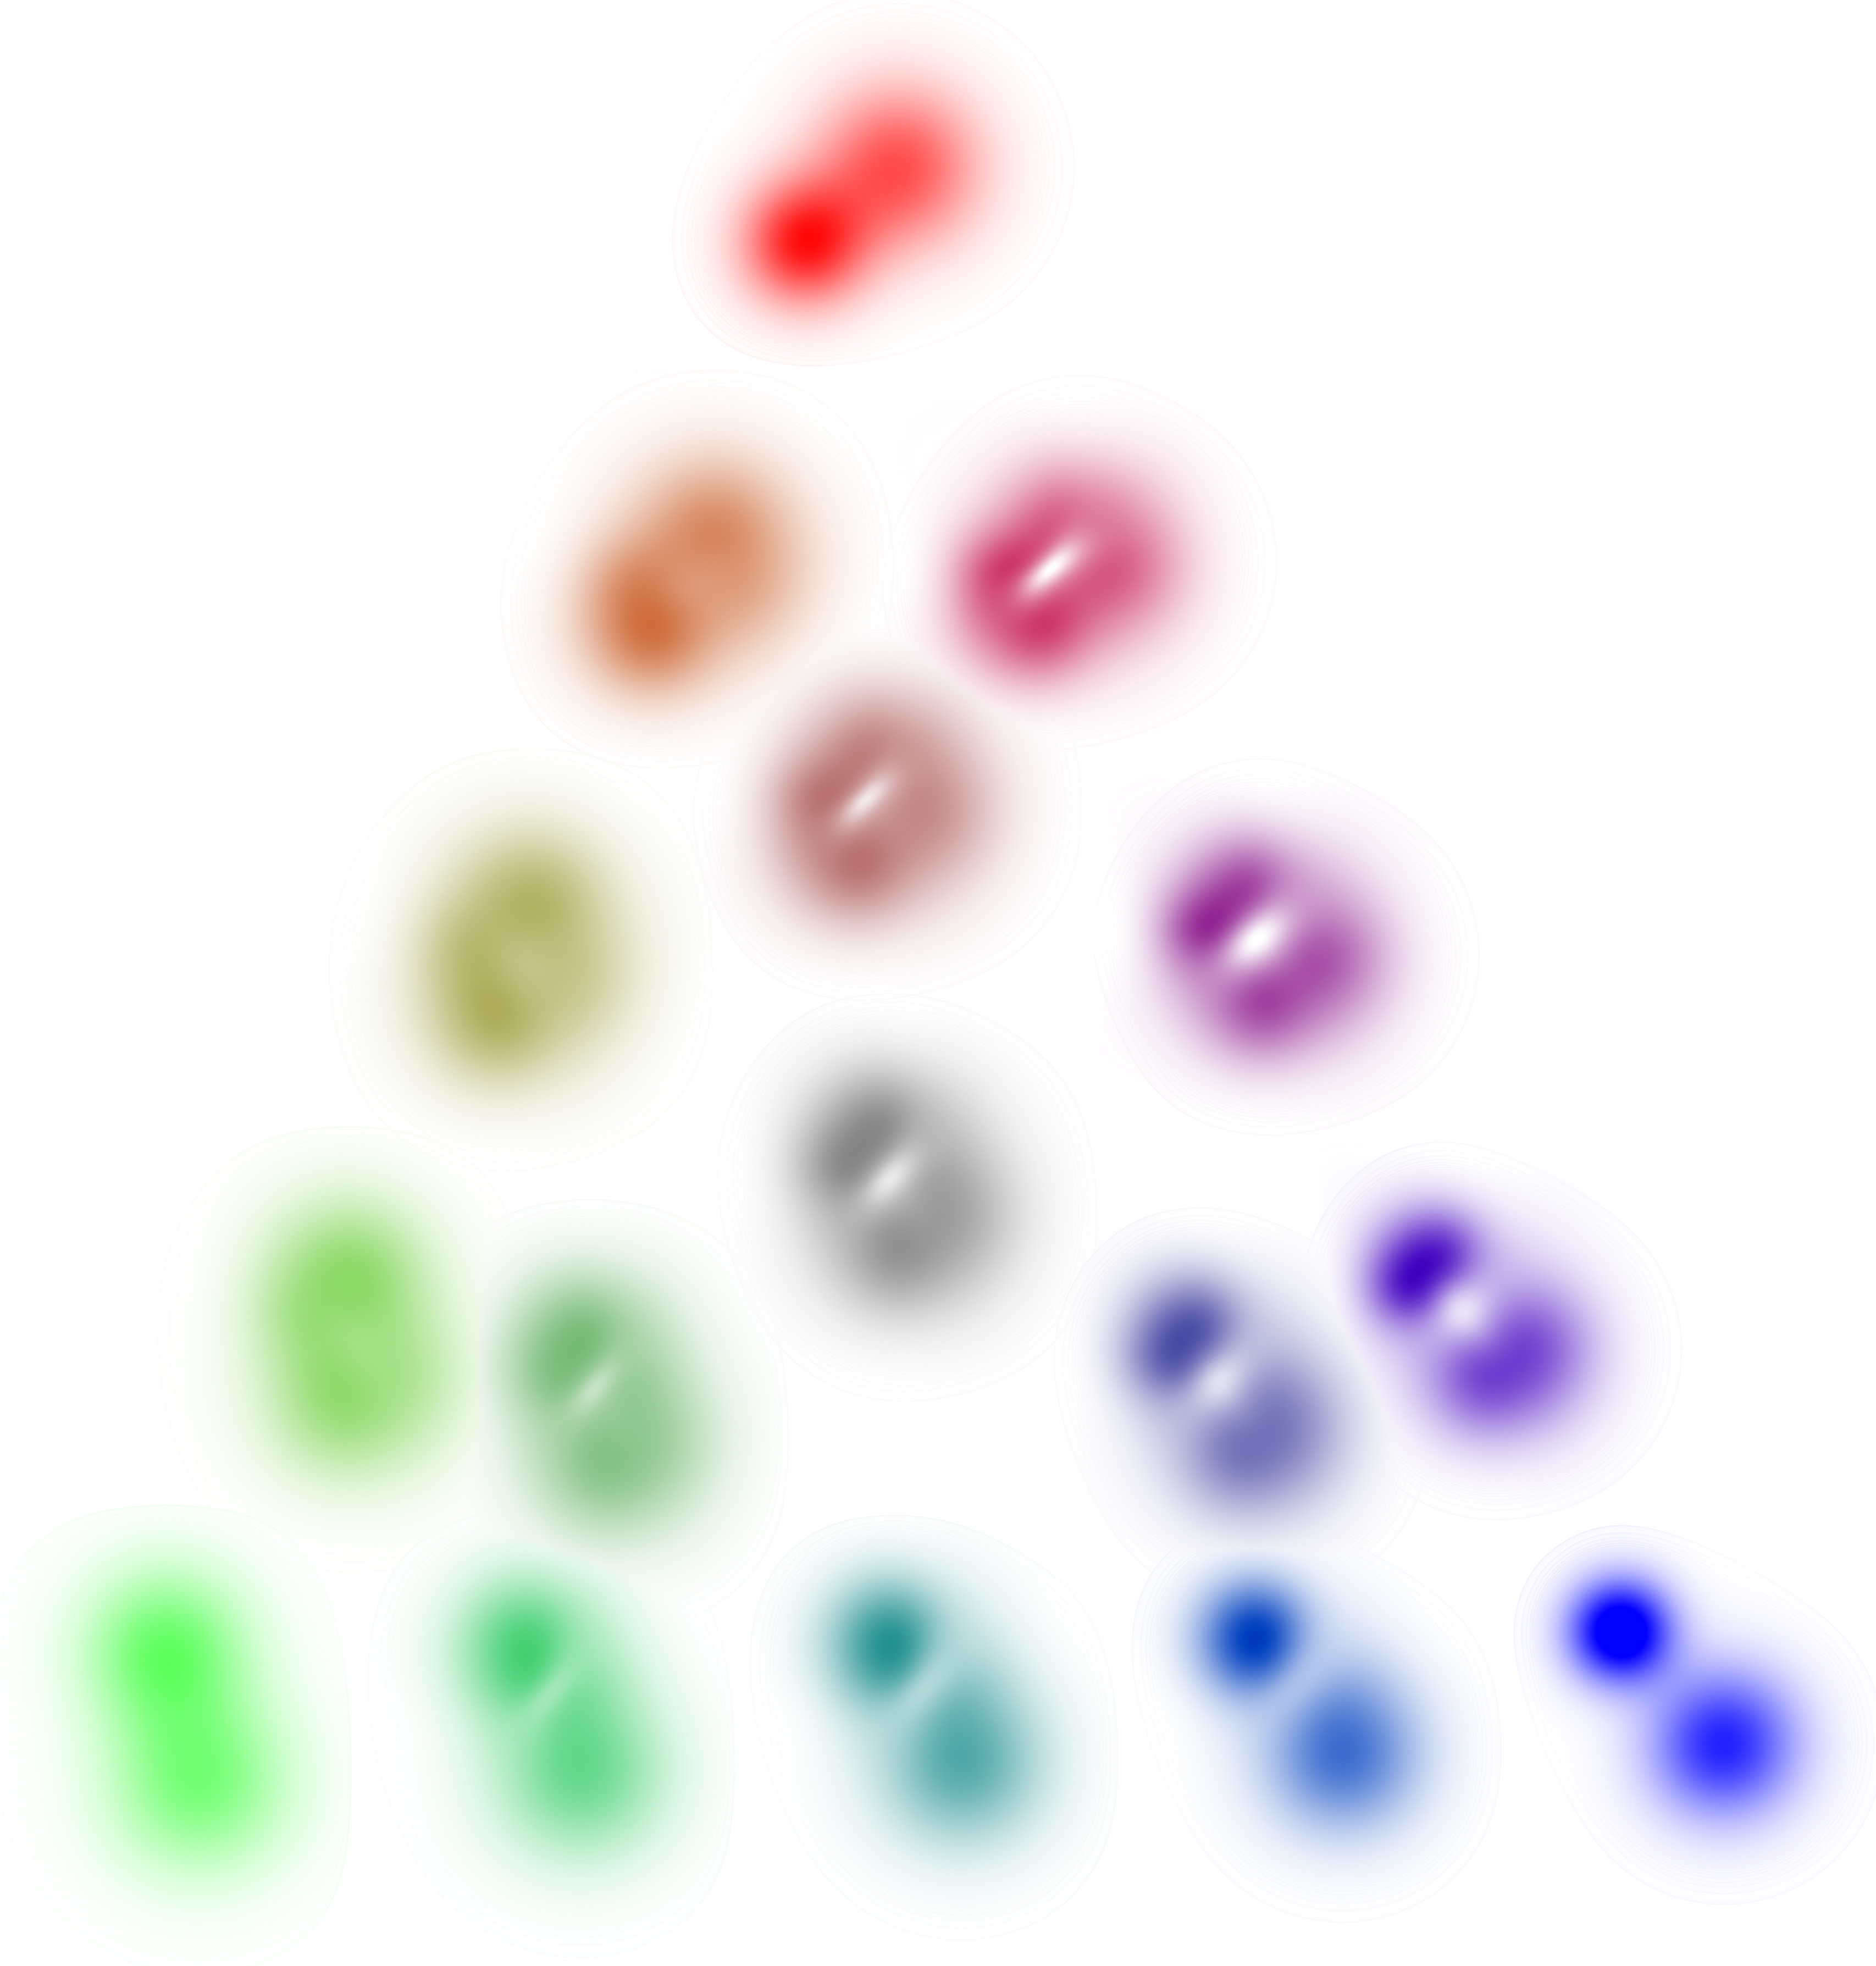
\includegraphics[width=0.31\linewidth]{twogauss/twogaussColorsFastSlant} &
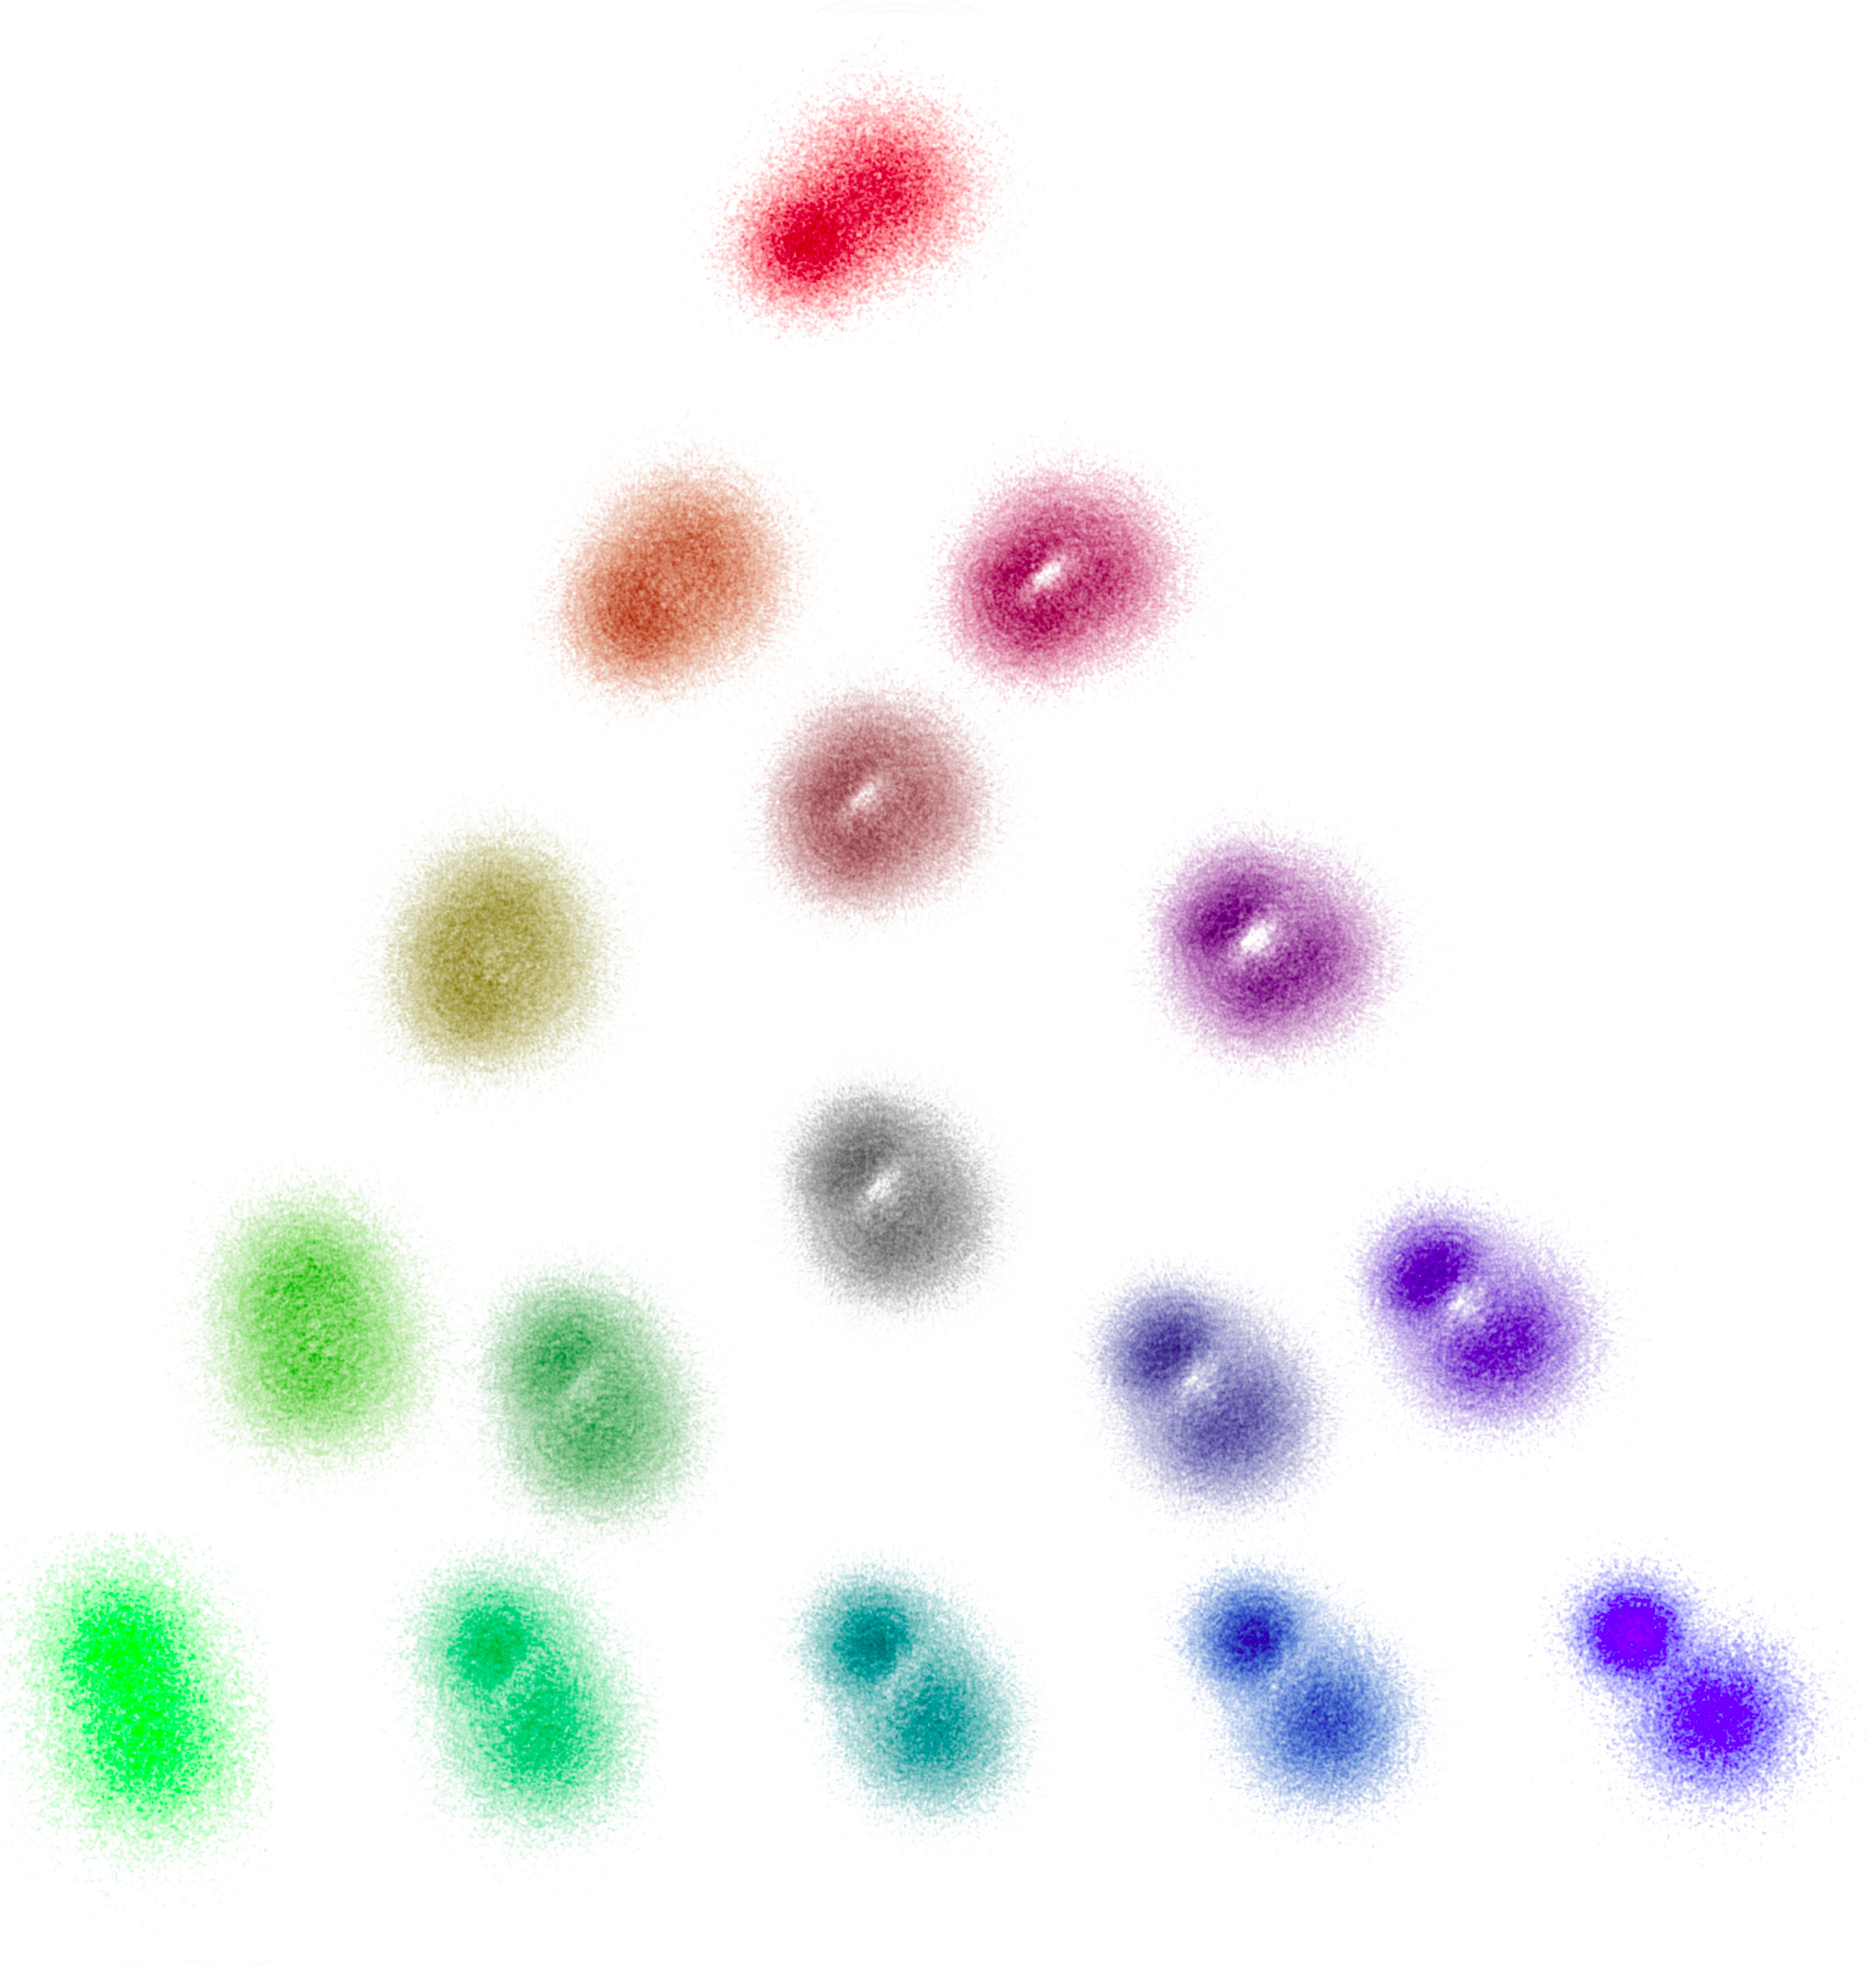
\includegraphics[width=0.31\linewidth]{twogauss/twogaussColorsSliced} &

\includegraphics[width=0.31\linewidth]{twogauss/twogaussColorsRef} \\
%\includegraphics[width=0.24\linewidth]{animals/animalsColorRadon_padded} &
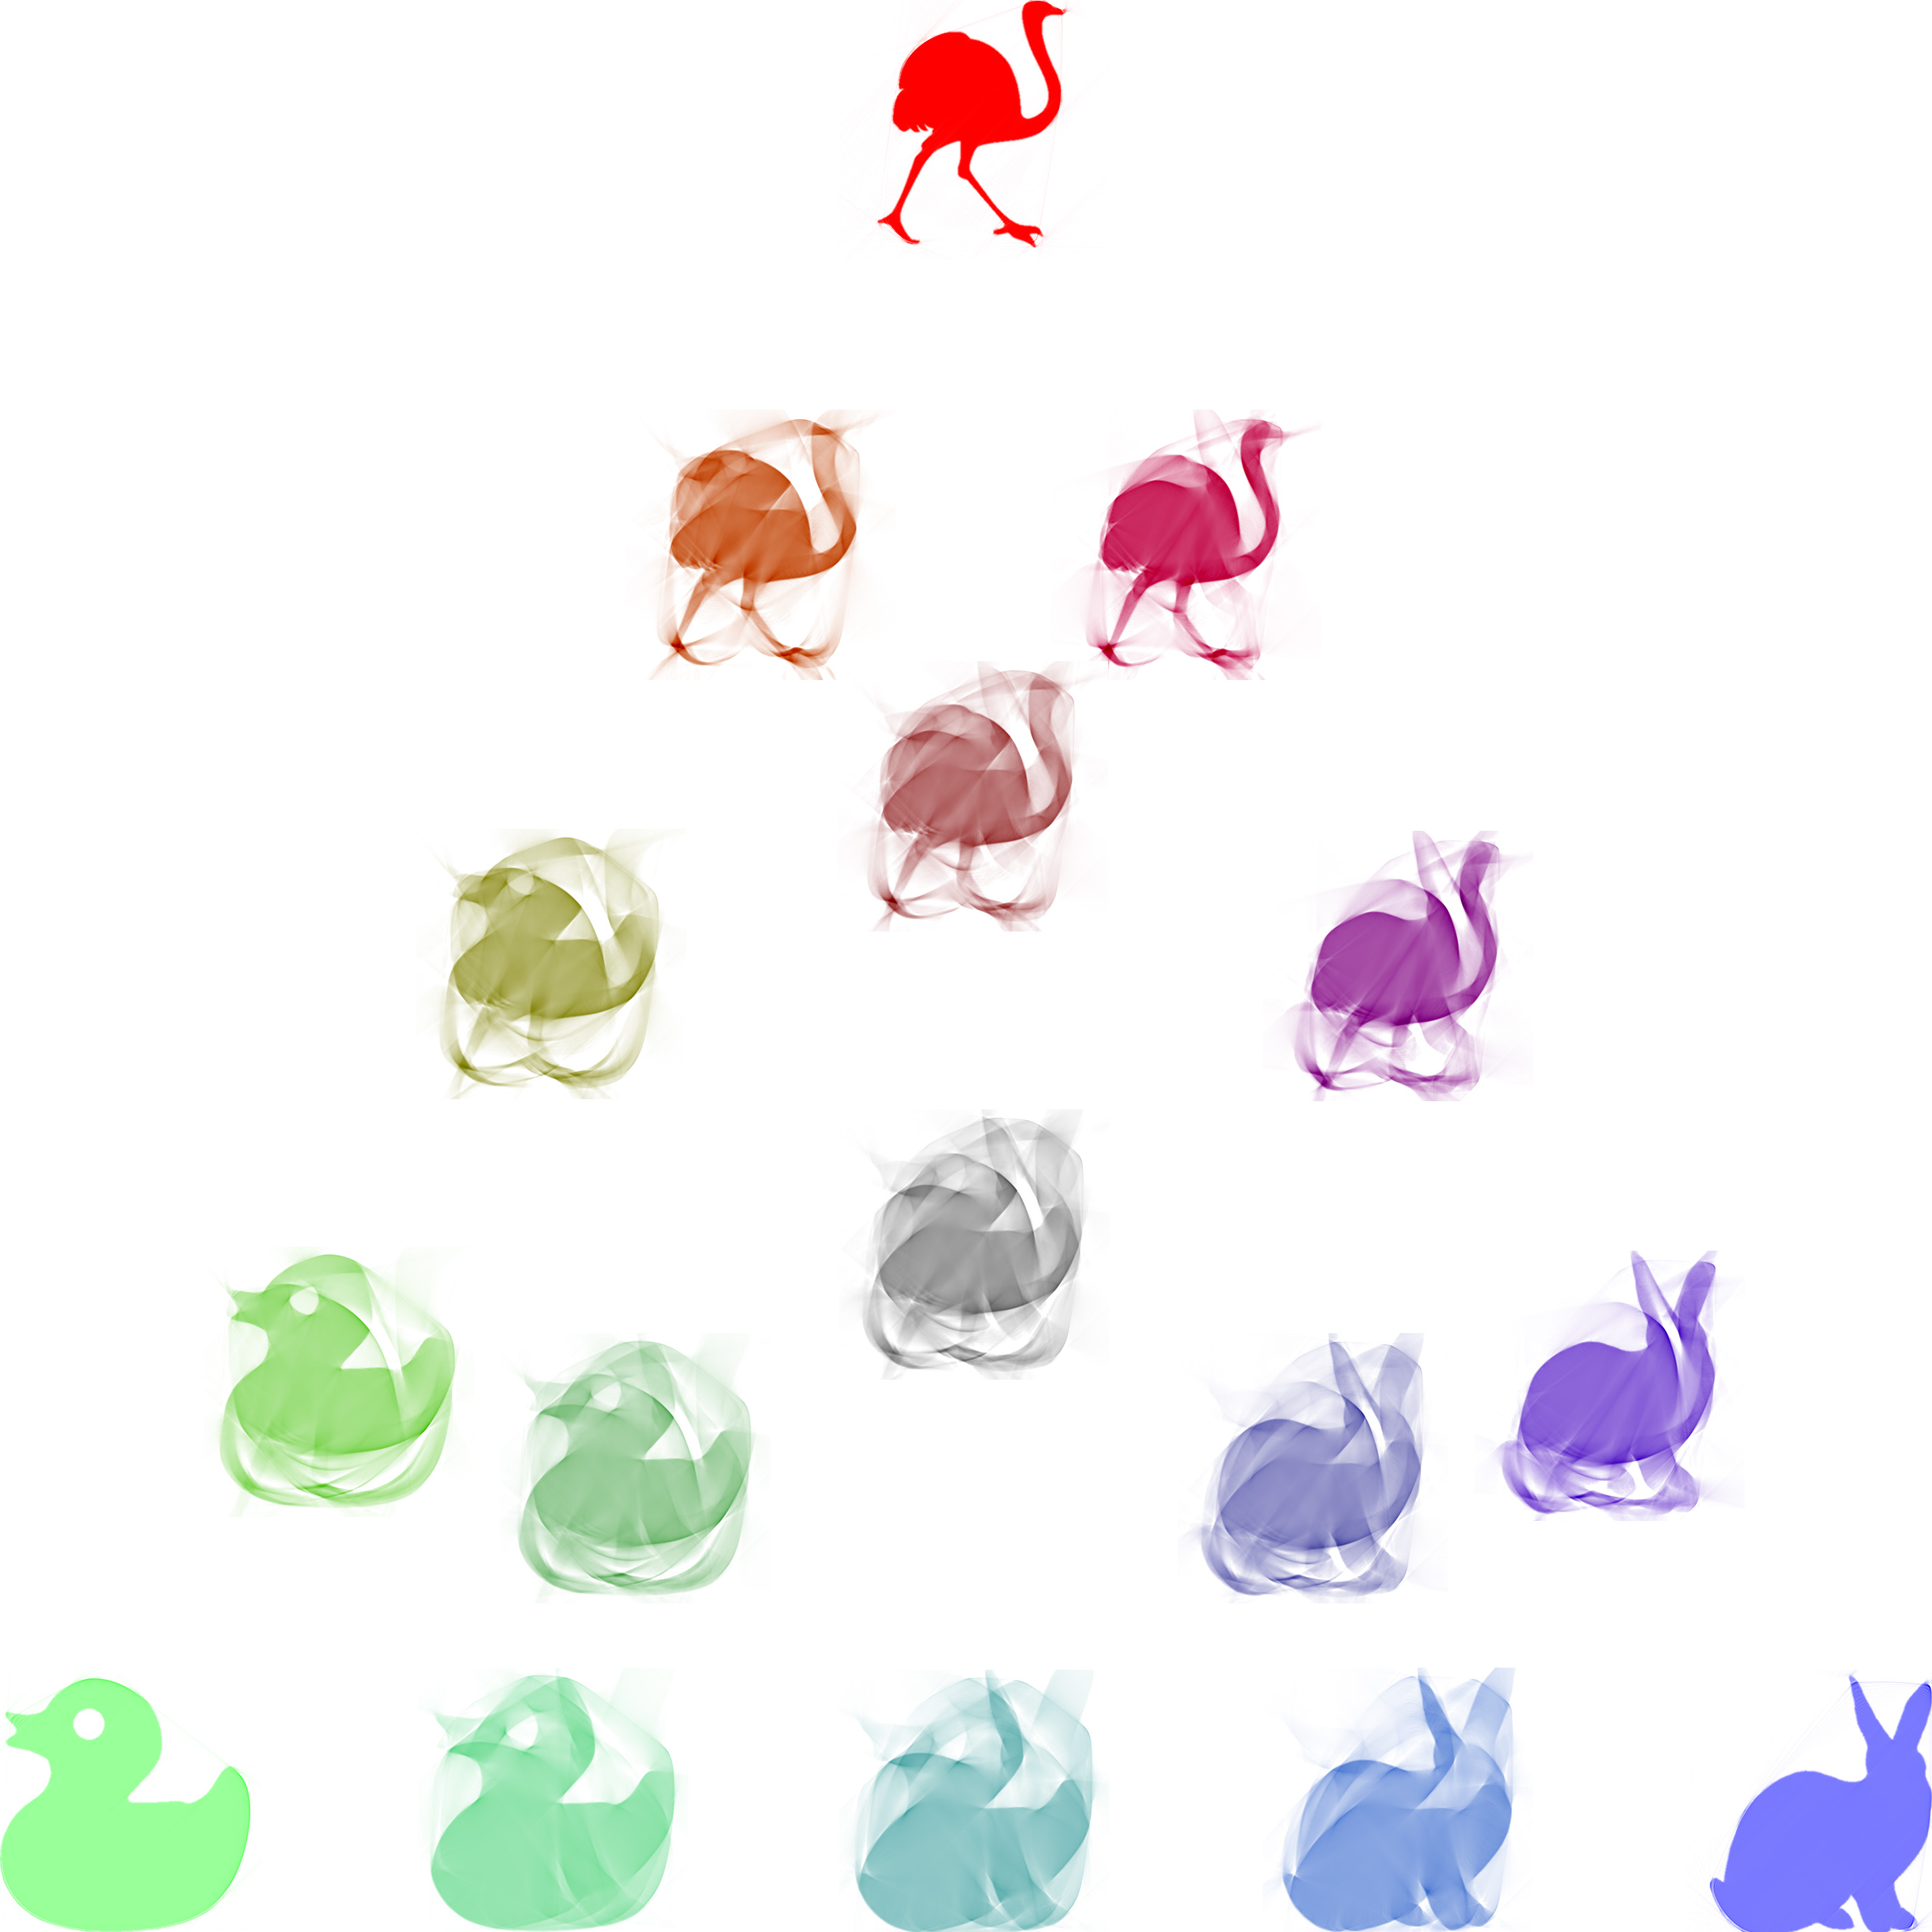
\includegraphics[width=0.31\linewidth]{animals/animalsColorFastSlant_padded} &
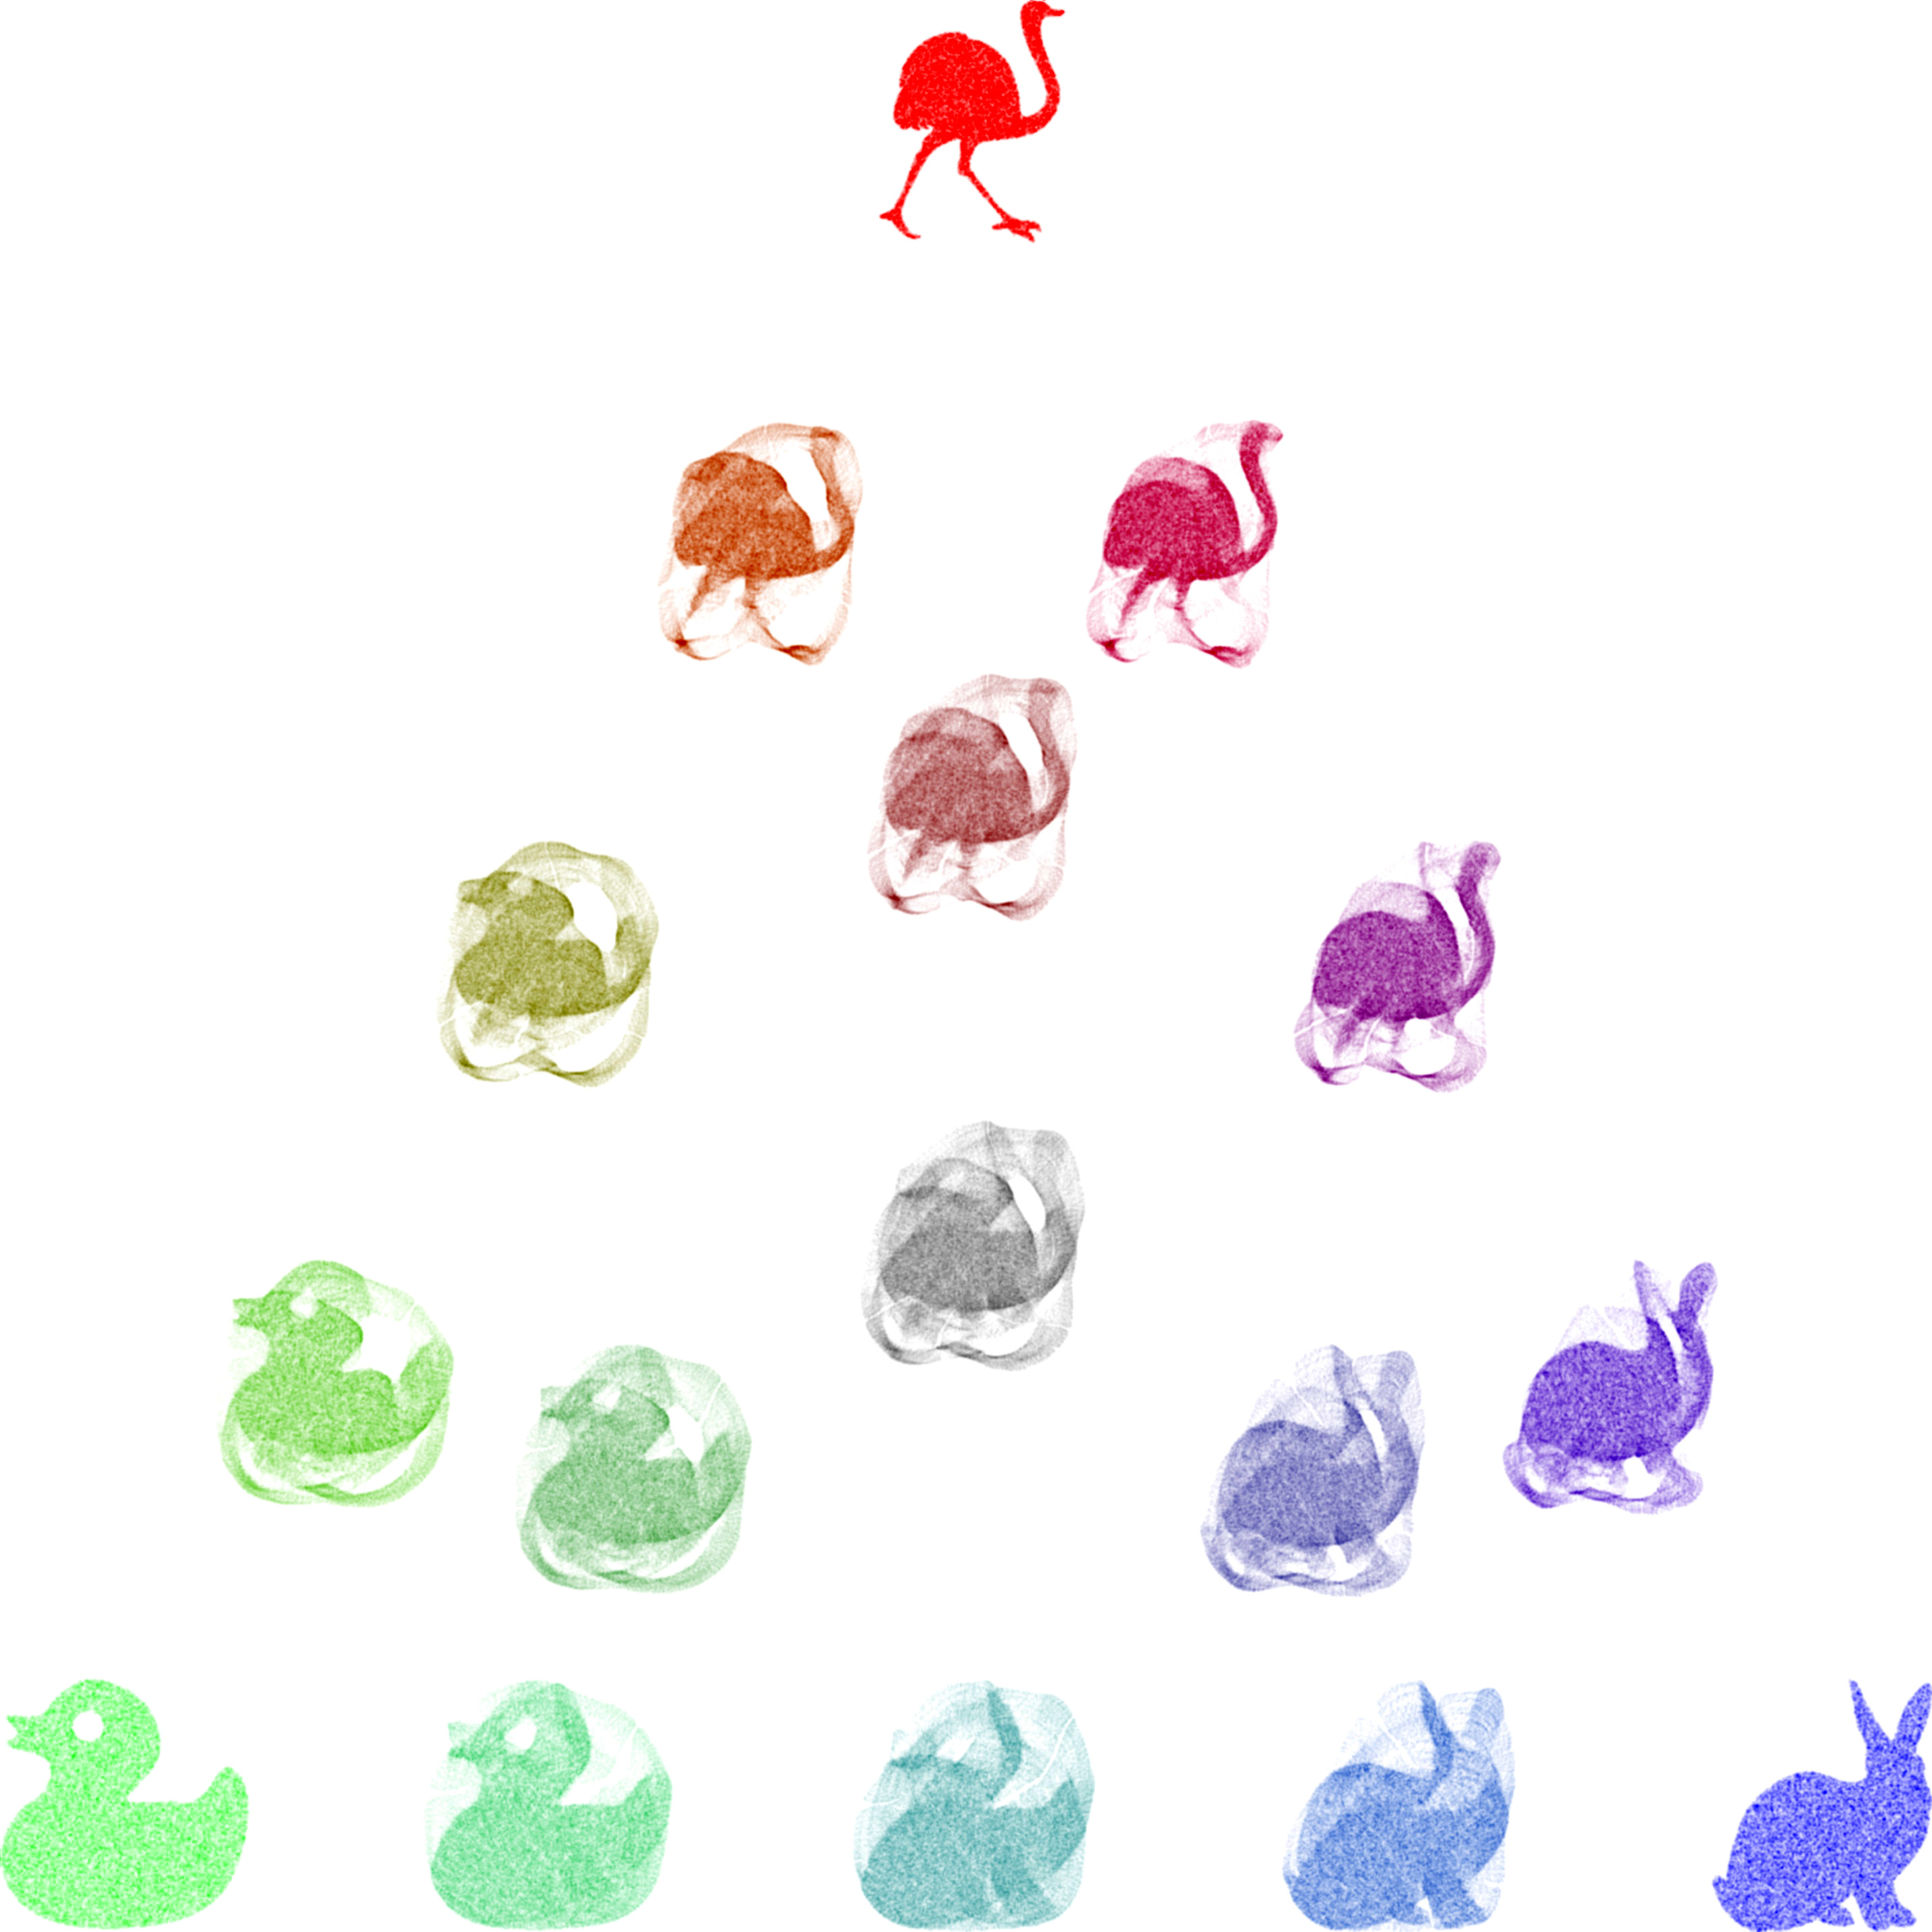
\includegraphics[width=0.31\linewidth]{animals/animalsColorSliced} &
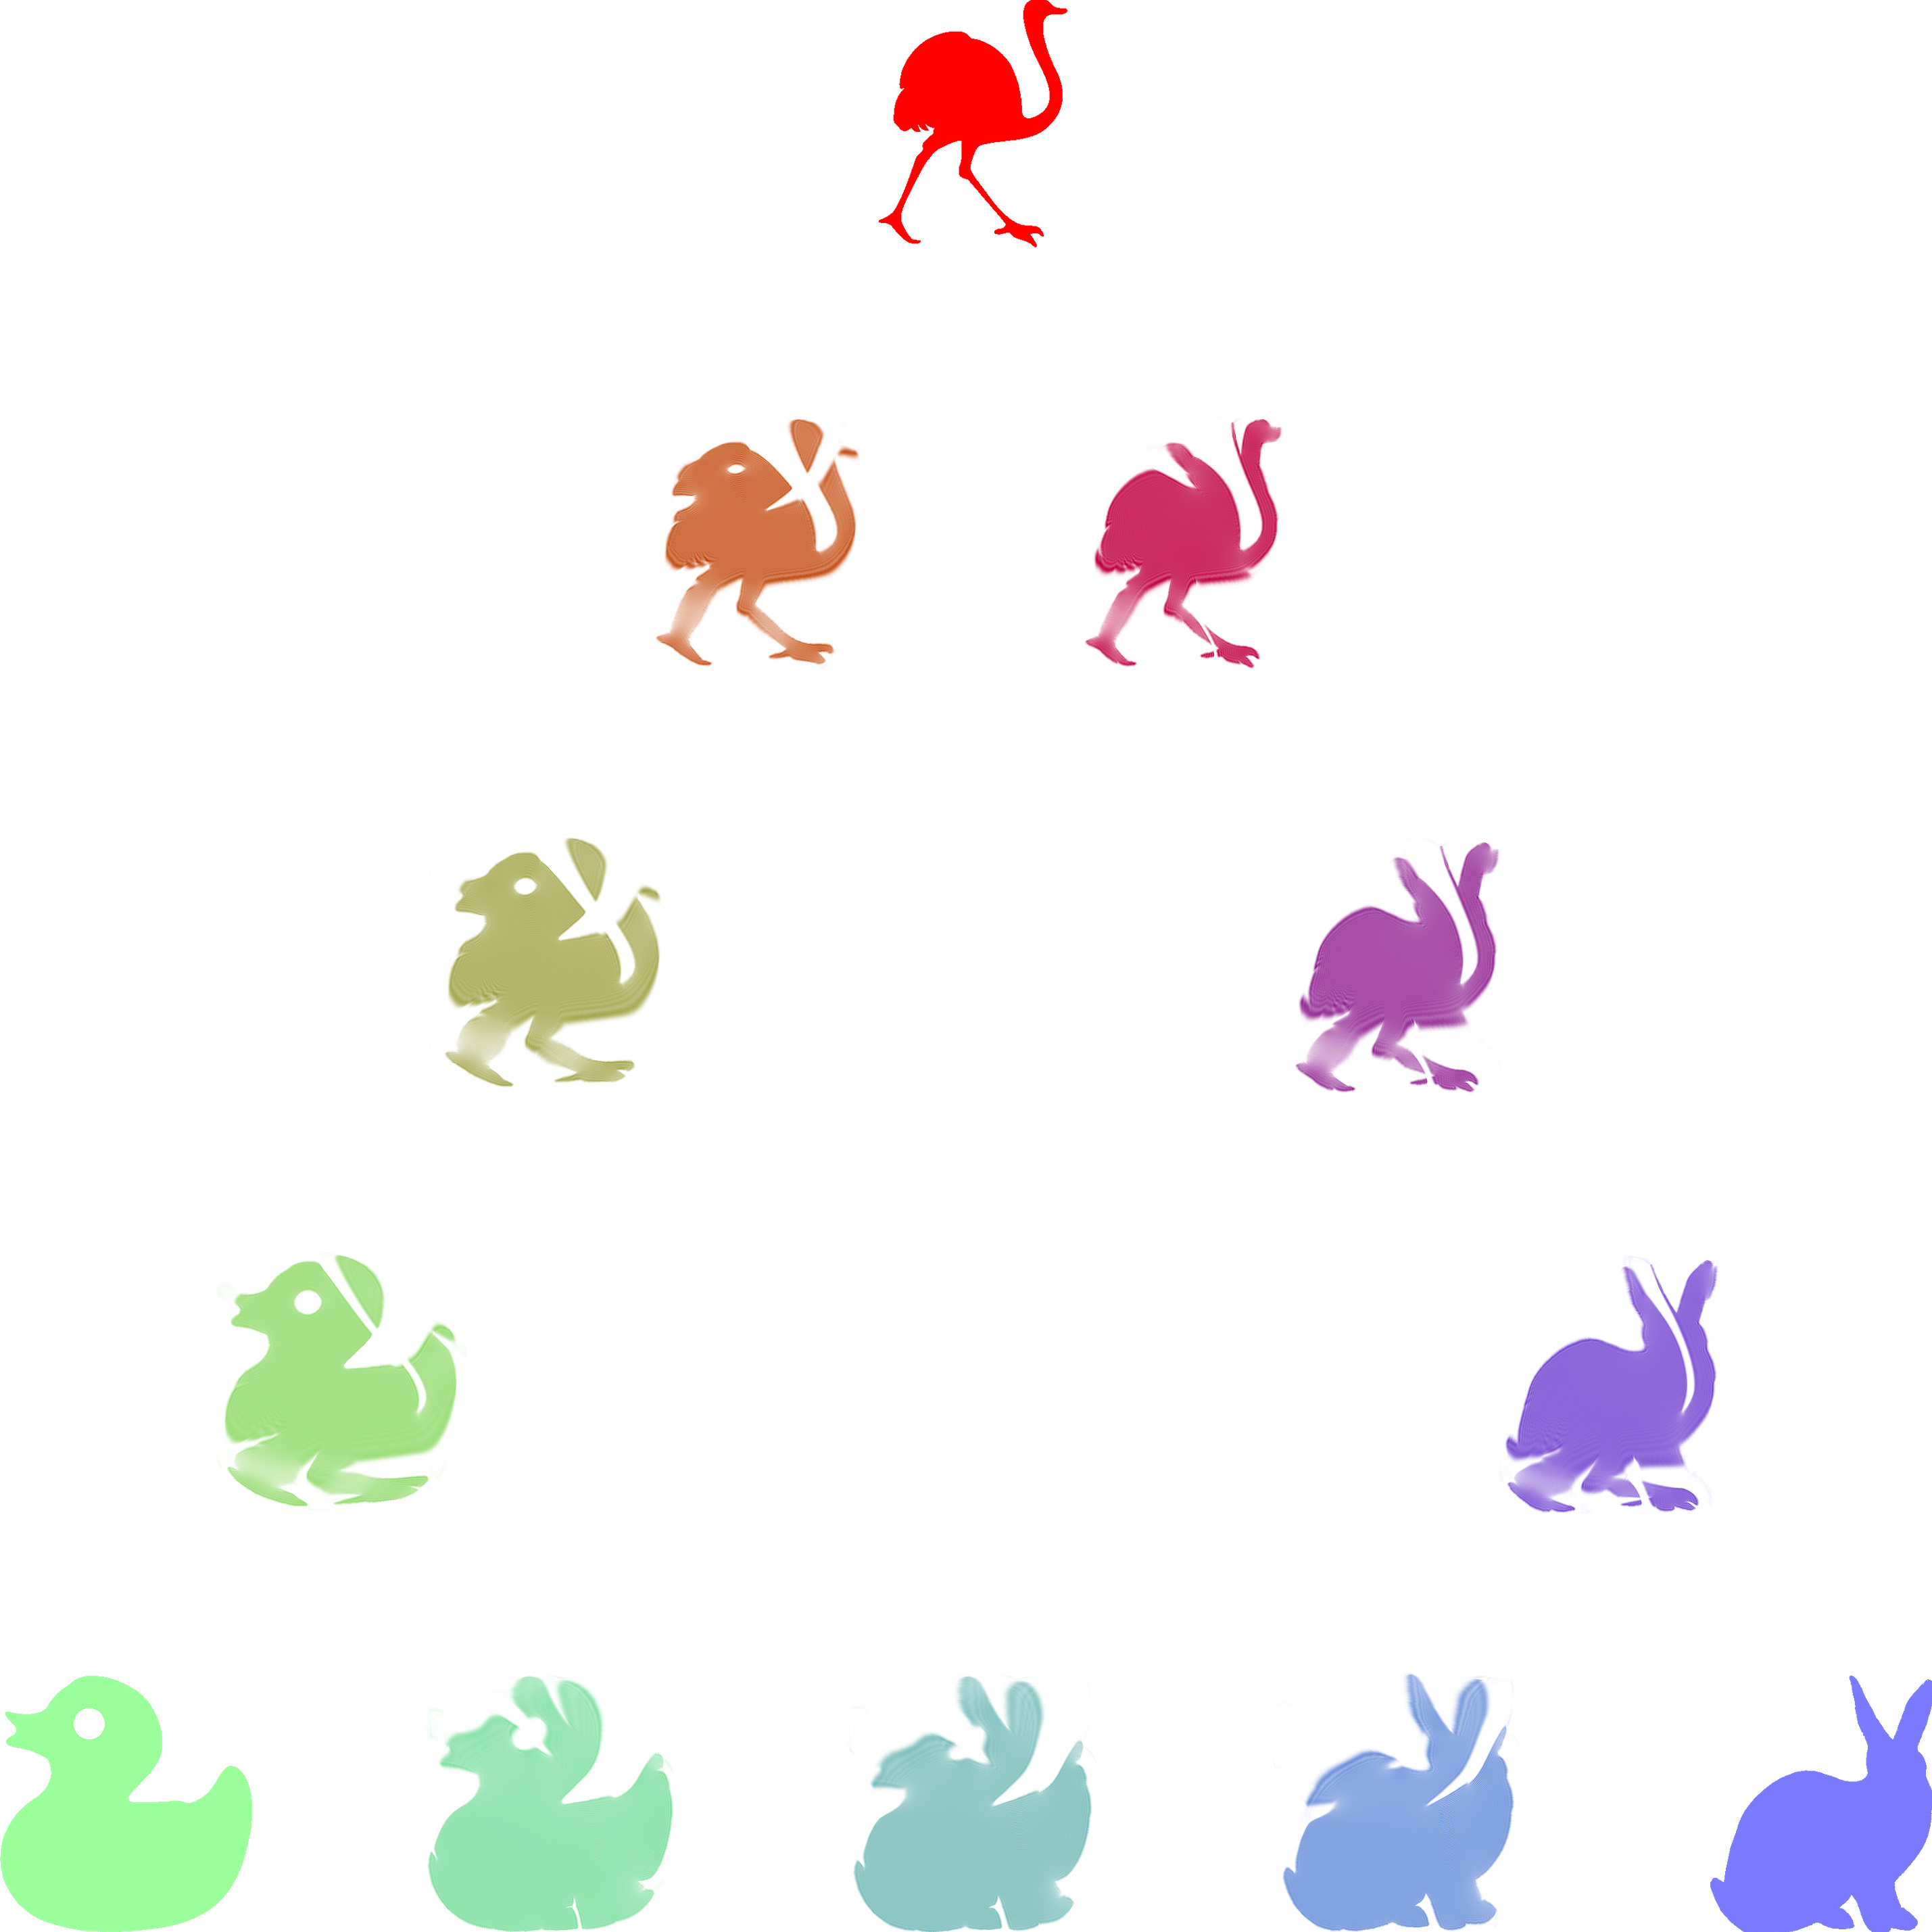
\includegraphics[width=0.31\linewidth]{animals/animalsColorRef} \\
 Radon barycenter  & Sliced barycenter & Wasserstein barycenter 
% & (b) Radon baryc. (Fast Slant Stack)
\end{tabular}
\end{center}
\caption{Comparison of $\Bary{\RR^d}^R, \Bary{\RR^d}^S$ and $\Bary{\RR^d}^W$ (computed using the method detailed in~\cite{FPapPeyOud13}).
}
\label{fig:compareRef}
\end{figure*}


%%%
\paragraph{Comparison of the Sliced and Radon barycenters.} 

As emphasized by Proposition~\ref{prop-comparison-bary}, while $\Bary{\RR^d}^R$ and $\Bary{\RR^d}^S$ are mathematically different, this difference is rather small, and is solely due to the lack of surjectivity of the Radon transform. We numerically evaluated this difference by computing 
\eq{
	\norm{ R(\Bary{\RR^d}^R(\mu_i, \lambda_i)_{i \in I}) - 
	\Bary{\Om^d}^W(R(\mu_i), \lambda_i)_{i \in I} }_{\text{TV}},
}
where $\norm{\cdot}_{\text{TV}}$ is the total variation of the measure defined in~\eqref{eq-tv-norm} and corresponds to the $L^1$ norm of the density in the case of an absolutely continuous measure. 
This measures the relative error due to the lack of surjectivity of $R$. Among several sets of discretized measures $\mu_i$ and weights $\lambda_i$, this relative error remained at approximately 0.15\%.
This said, the main difference between the sliced and Radon barycenter lies in their discretizations: $\Bary{\RR^d}^R$ is approximated with an Eulerian scheme and $\Bary{\RR^d}^S$ with a Lagrangian scheme.

\begin{figure}[!t]
\begin{center}
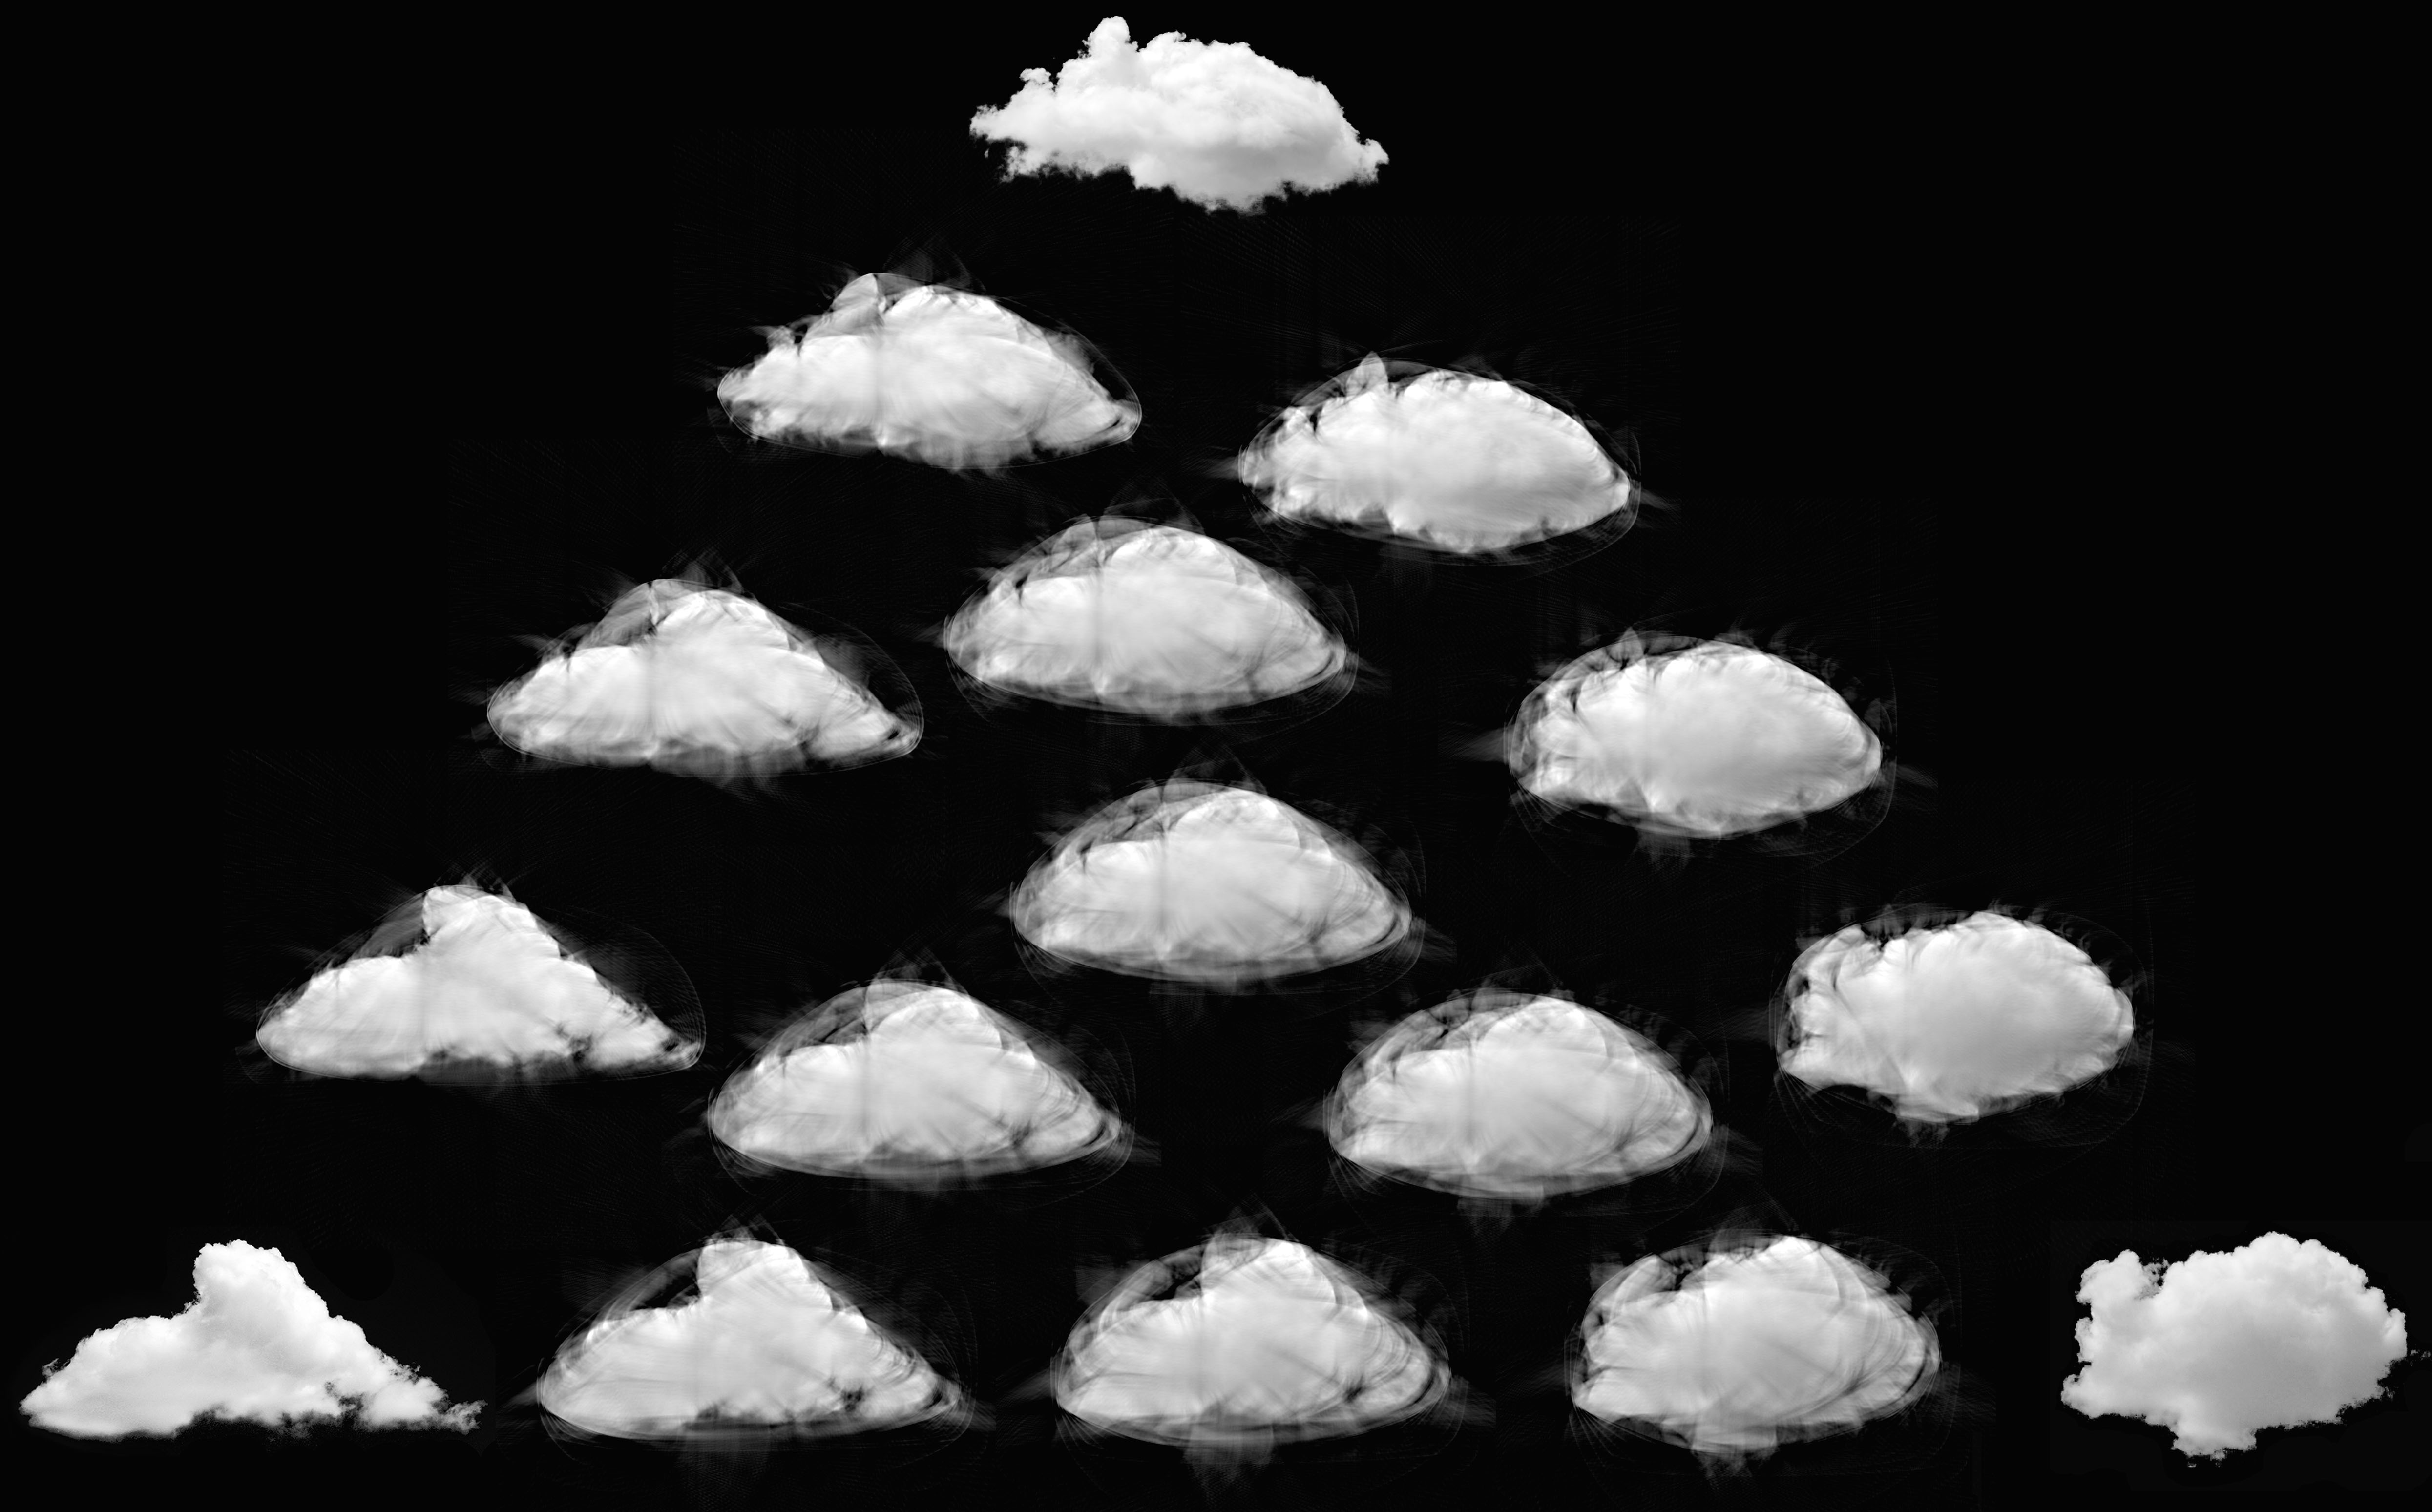
\includegraphics[width=\linewidth]{clouds/clouds.jpg}
\end{center}
\caption{Image warping using the Radon barycenter exhibits artifacts.  }
\label{fig:cloud}
\end{figure}


Figure~\ref{fig:compareRef} shows that the discretized barycenters are quite similar when computing the barycenter of three measures. Figure~\ref{fig:bary4} shows a similar comparison for the iso-barycenter of four measures. Figure~\ref{fig:cloud} shows what could be considered as a failure of the method to adapt to the computation of complex image barycenters. 

\begin{figure}[!t]
\begin{center}
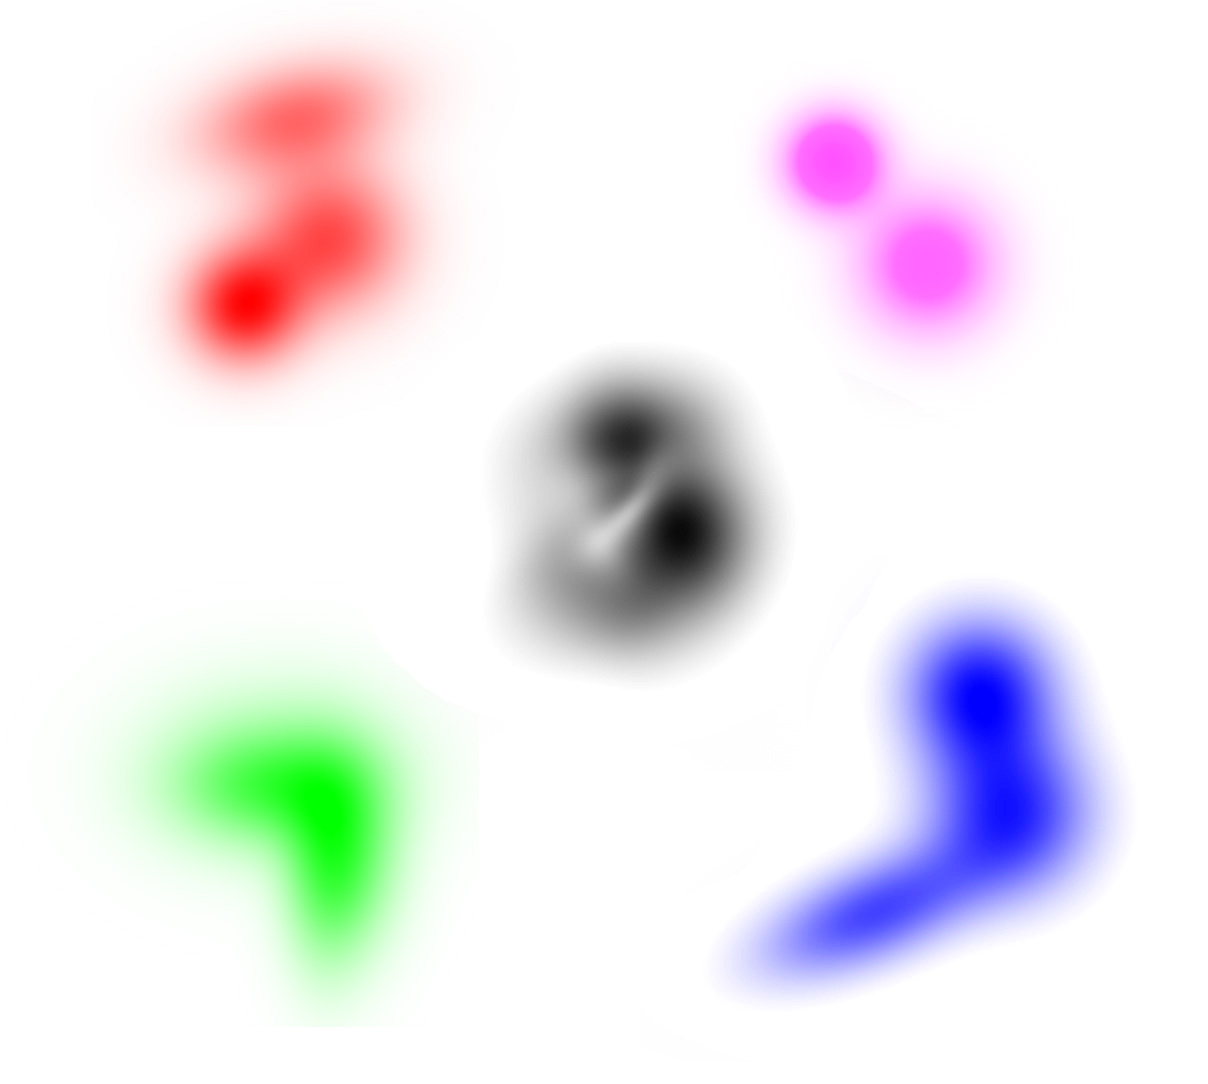
\includegraphics[width=0.48\linewidth]{bary4/bary4_padded}
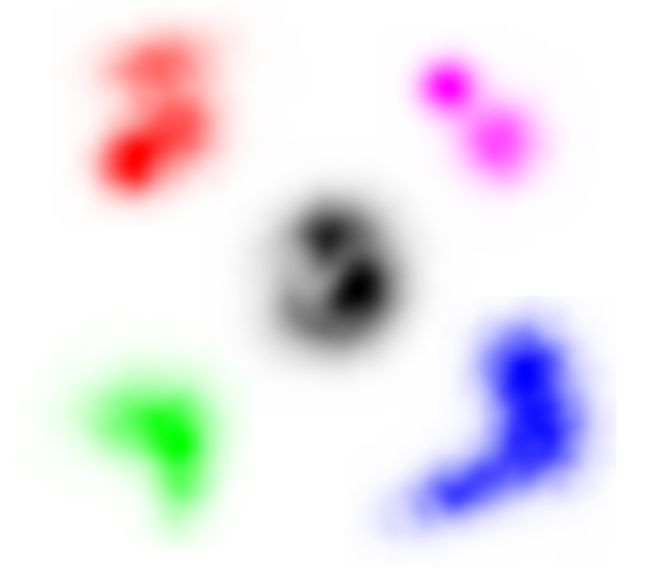
\includegraphics[width=0.48\linewidth]{bary4/bary4_SW2_100dir_40kpoints_sig20_N512pix}
\end{center}
\caption{Top: Radon barycenter $\Bary{\RR^d}^R$ of four 2-D distributions with equal weights. 
Bottom : Same experiment with SW2, using $N=4\,10^4$ points samples, $|\Theta|=100$ directions and a gaussian kernel with standard deviation $\sigma=20/512$ to estimate the corresponding densities. .
}
\label{fig:bary4}
\end{figure}


%%%
\paragraph{Comparison of computational complexity.}

A typical Radon barycenter of three two-dimensional pdfs discretized on a $1024 \times 1024$ pixel grid, and the principled Fast Slant Stack Radon transform with $2048$ slices, requires $11$ seconds to precompute the initial Radon transforms, and $170$ seconds to compute $32$ Radon barycenters, with unoptimized parallel Matlab code. It is possible to accelerate this timing using less precise Radon transform. For instance, using Matlab's implementation of the Radon transform with $180$ slices requires $14$ seconds to compute these $32$ barycenters on a single core. 
In comparison with the Eulerian proximal splitting method of Papadakis et al.~\cite{FPapPeyOud13}, the Wasserstein barycenter between two $1024 \times 1024$ distributions with $32$ time steps and $100,000$ iterations to achieve an acceptable convergence requires on average 72 hours, using an optimized C++ vectorized and parallel implementation (see Fig.~\ref{fig:compareRef} for a display of the resulting barycenters).

A sliced barycenter of three distributions, each approximated with 40k Dirac masses and 100 directions, requires 140 seconds using 100 iterations of Newton descent or 18 seconds using the stochastic Newton descent with subsets of 10 directions. With a finer set of 1000 directions and the same setup, the stochastic Newton descent with subsets of 100 directions requires 168 seconds.


%%%
\paragraph{Comparison with the entropy regularized barycenter~\cite{CuturiBarycenter}.}

Cuturi and Doucet proposed in~\cite{CuturiBarycenter} a method to approximate the Wasserstein barycenter on a fixed grid, hence using the Eulerian discretization presented in Section~\ref{subsec-algorithm-eulerian}. Their method performs a gradient descent on a smoothed Wasserstein distance. This smoothing is obtained by adding an entropic penalization to the linear cost function~\eqref{eq-dfn-wass-dist} defining the transportation distance. Figure~\ref{fig:compareMarco} shows a visual comparison of the iso-barycenters computed with this approach as well as with the sliced and Radon methods. 

The result obtained with the method of~\cite{CuturiBarycenter} is produced in two hours on a GPU, using a $150 \times 150$ sampling grid. In contrast, our Radon barycenter computed on a grid of $400 \times 400$ pixels (which is zero-padded to $1200 \times 1200$ pixels to avoid Radon transform artifacts) is obtained in 40 seconds using the fast slant stack approach with 1200 directions, and 2 seconds with Matlab built-in Radon transforms with 180 directions, on a single core of a laptop. Similarly, our Sliced barycenter implemented in Matlab produced the interpolation in 20 minutes, using $4 \times 10^5$ points sampled on a interpolated grid of $1000 \times 1000$ pixels, with 100 directions and 100 iterations.

\begin{figure}[!ht]
\begin{center} 
\begin{tabular}{c@{\hspace{1mm}}c@{\hspace{1mm}}c@{}}
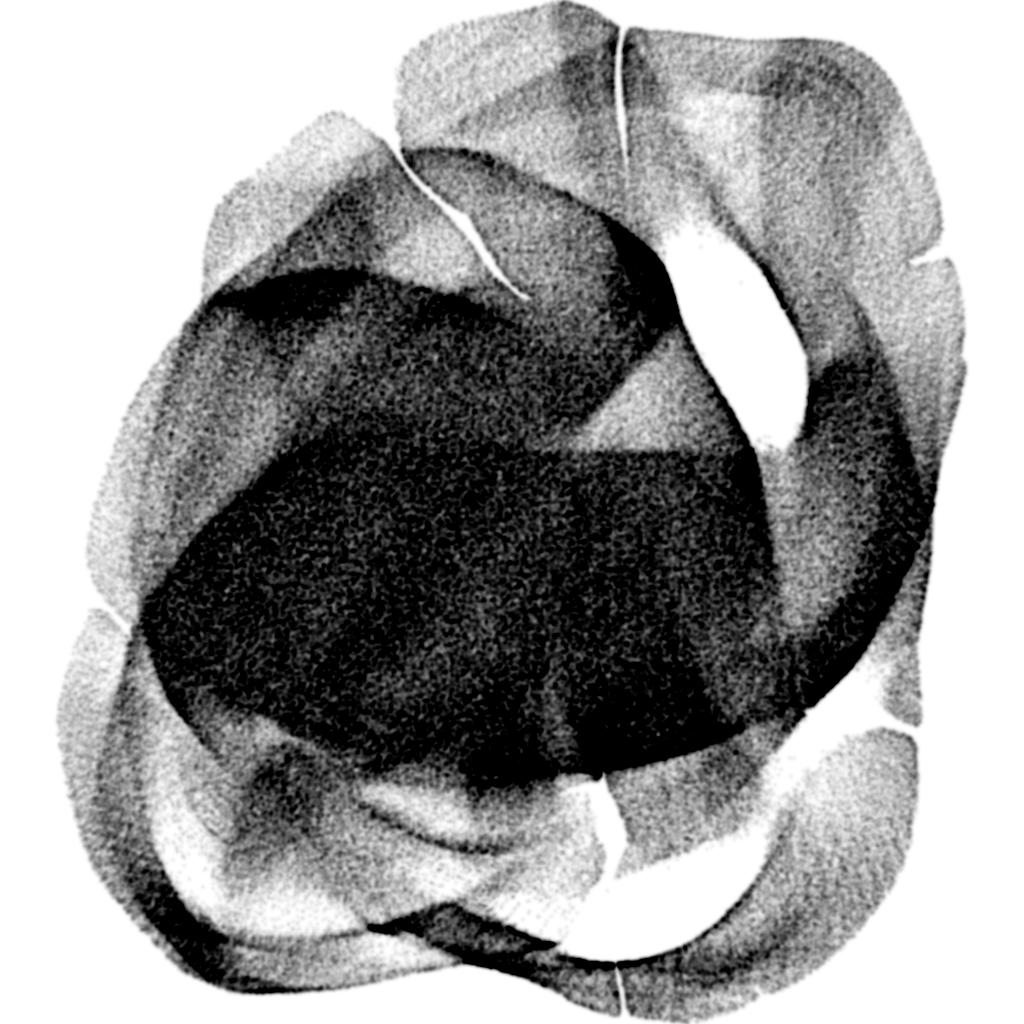
\includegraphics[width=.32\linewidth]{cuturi/bary-animals-Sliced-1-1-1_thresh} &
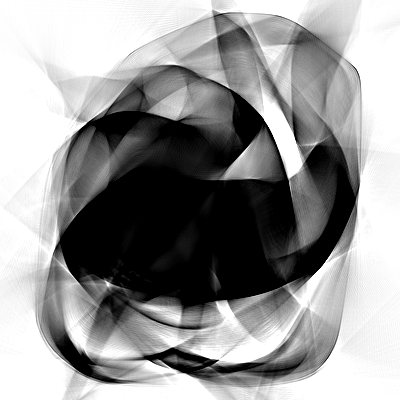
\includegraphics[width=.32\linewidth]{cuturi/animal_padded111} &

\includegraphics[width=.32\linewidth]{cuturi/bary-animals-cuturi-1-1-1} \\
$\Bary{\RR^d}^S$ & $\Bary{\RR^d}^R$ & Cuturi et al.
\end{tabular}
\end{center}
\caption{Comparison of three methods (Sliced, Radon, and the one presented in~\cite{CuturiBarycenter}) to compute isobarycenters (i.e. using $\la=(1,1,1)/3$) of the three input densities displayed at the vertices of Figure~\ref{fig:compareRef}, bottom. 
}
\label{fig:compareMarco}
\end{figure}


%%%%%%%%%%%%%%%%%%%%%%%%%%%%%%%%%%%%%%%%%%%%%%%%%%%
\subsection{Application to Texture Mixing} 

To illustrate the usefulness of the Radon barycenter, we apply it to the problem of texture mixing. The Radon barycenter is well suited to this application which requires an Eulerian discretization in order to interpolate power-spectra computed on the uniform grid of Fourier frequencies. This would be hardly feasible using the Lagrangian discretization of the Sliced barycenter. 


%%%%%
\paragraph{Texture mixing.}

Given a set of input texture images $\{ f^{[i]} \}_{i \in I}$, where each $f^{[i]} \in \RR^N$ is a grayscale image of $N=n \times n$ pixels, the goal of texture mixing is to produce a set of random vectors $\{ F^{[i]} \}_{i \in I}$, and an interpolation method $\la \in \La_I \mapsto F_\la$. In particular, it means that if $\la$ is $0$ excepted at the $i^{\text{th}}$ coordinate, then $F_\la=F^{[i]}$ (interpolation at the vertices of the simplex indexed by $I$). Texture mixing is a generalization of texture synthesis (which simply corresponds to the case $|I|=1$), in the sense that any realization $\tilde f^{[i]}$ of the random vector $F^{[i]}$ should look both ``random'' and visually similar (but not equal) to the input $f^{[i]}$.


%%%%%
\paragraph{Spot-noise (SN) texture model.}

Following the work of~\cite{galerne-ieee} (which introduces the name ``spot noise'' model), we consider stationary Gaussian random vectors $F$ which take values in $\RR^N$. These vectors are indexed on the image grid 
\eq{
	F = (F_k)_{k \in \Gg}
	\qwhereq
	\Gg = \{-n/2+1, \ldots, n/2\}^2, 
}
(for simplicity we assume that $n$ is even) and we use periodic boundary conditions. Without loss of generality, we assume that they have zero mean $\EE(F)=0$. 
% and unit global variance $\EE(\norm{F}^2)=1$. Note the mean and the variance are usually adjusted to match the contrast of the display. 
Such a random vector is thus entirely characterized by its (square root) power spectrum density (PSD)
\eq{
	\foralls \om \in \Gg, \quad P_F(\om) = \EE( |\hat F(\om)|^2 )^{1/2} 
}
where we define the Fourier transform of a vector or a random vector as
\eq{
	\foralls \om \in \Gg, \quad
	\hat F(\om) = \sum_{k \in \Gg} F_k e^{\frac{2 \imath \pi}{n} \dotp{k}{\om} }
}
\eq{
	\qwhereq
	 \dotp{k}{\om} = k_1 \om_1 + k_2 \om_2.
} 
We remind that once the power-spectrum $P_F$ of $F$ is known, $F$ is recovered by 
\eql{\label{eq-gaussian-sampling}
	\hat F(\om) = P_F(\om) \cdot \hat W(\om)
	\qwhereq
	W \sim \Nn(0,\Id_{N}).
}
It is thus easy to draw a realization $f$ of the vector $F$ by convolving the inverse Fourier transform of $P_F$ (the so-called texton, see~\cite{Desolneux-Moisan-12}) by a realization $w$ of the white noise $W$, i.e., computing $\hat f = P_F \cdot \hat w$, where $\cdot$ denotes entry-wise multiplication.


In this spot noise model, it is customary (see~\cite{galerne-ieee}) to learn the input Gaussian models $\{F^{[i]}\}_{i \in I}$ by estimating their PSD with a maximum likelihood estimation, which corresponds to estimating the covariance using the empirical periodogram
\eq{
	\foralls i \in I, \quad \foralls \om \in \Gg, \quad
	P_{F^{[i]}}(\om) = |\hat f^{[i]}(\om)|. 
} 
We also use this estimation, which, despite its simplicity, gives good visual performances, see~\cite{peyre2013Gaussians}. 

%%%%%
\paragraph{Optimal transport barycenter of SN models.}

We introduce a texture mixing method that performs the interpolation of the PSD using optimal transport. The rational of this method is to operate the mixing with geometric warpings of the spectral modes of the textures. The method is thus adapted to deal with micro-textures which exhibit a high degree of sparsity in the Fourier domain, i.e., which PSD are composed of a few localized spikes. This class of sparse spectral textures has been shown in~\cite{GalerneGabor} to be a powerful way to approximate more complicated textures for procedural texture synthesis. 

We define the measure associated to the PSD of the Gaussian model $F^{[i]}$ 
\eq{
	\foralls i \in I, \quad
	\mu_i = \frac{1}{\sum_{\om \in \Gg} P_{F^{[i]}}(\om)} 
		\sum_{\om \in \Gg} P_{F^{[i]}}(\om) \de_{\om} \in \Mm_1^+(\RR^2).
}
The barycenter measure is defined as
\eq{
	\foralls \la \in \La_I, \quad
	\mu^{(\la)} = \Bary{\RR^2}^R( \mu_i, \la_i )_{i \in I}.
}
Note that this measure exhibits central symmetry because of~\eqref{eq-prop-inv-cent} and Proposition~\eqref{prop:InvarianceHolds}.

This barycenter measure is approximated using the Eulerian discretized Radon barycenter described in Section~\ref{subsec-algorithm-eulerian}, to obtain a resulting measure 
\eq{	
	\bar\mu^{(\la)} = \Bary{\Gg}^R( \mu_i, \la_i )_{i \in I}.
}
By construction of this algorithm, this measure is supported on the grid $\Gg$ and also exhibits central symmetry. It can thus be written as
\eq{
	\bar\mu^{(\la)} = \sum_{\om \in \Gg} P_{F_\la}(\om) \de_{\om}.
}
This thus defines a stationary Gaussian random vector $F_\la$ through its PSD $P_{F_\la}$. This Gaussian vector is our interpolated model, which can be synthesized following~\eqref{eq-gaussian-sampling}. 


%%%%%
\paragraph{Examples.} 

We demonstrate our Radon barycenter of power spectrum densities on several examples. A sparse hand-de\-si\-gned power spectrum is interpolated in Fig.~\ref{fig:texsynth} and a more natural, less sparse, power spectrum is used in Fig.~\ref{fig:texsynth2}.
We handle colors by convolving the interpolated power spectrum of each color channel by the same white noise. Although the decoupling of color channels could occasionally lead to color artifacts, we did not 
observe such effects on our set of examples (further examples can be see in the additional material). We hence leave the investigation of perceptually decoupled color spaces 
or the joint transportation of color channels for future work.
%\todo{Then it means you treat each channel independently and do barycenter for each channel ? I thought this would leads to color artifact since you do not model the cross correlation between the channels. This needs clarification. }.

%\todo{Detail a bit, in particular how to handle colors}


\begin{figure*}[!t]
\setlength{\tabcolsep}{0pt}
  \setlength{\fboxsep}{0pt}
\begin{center} 
\begin{tabular}{@{}c@{\hspace{1mm}}c@{}}
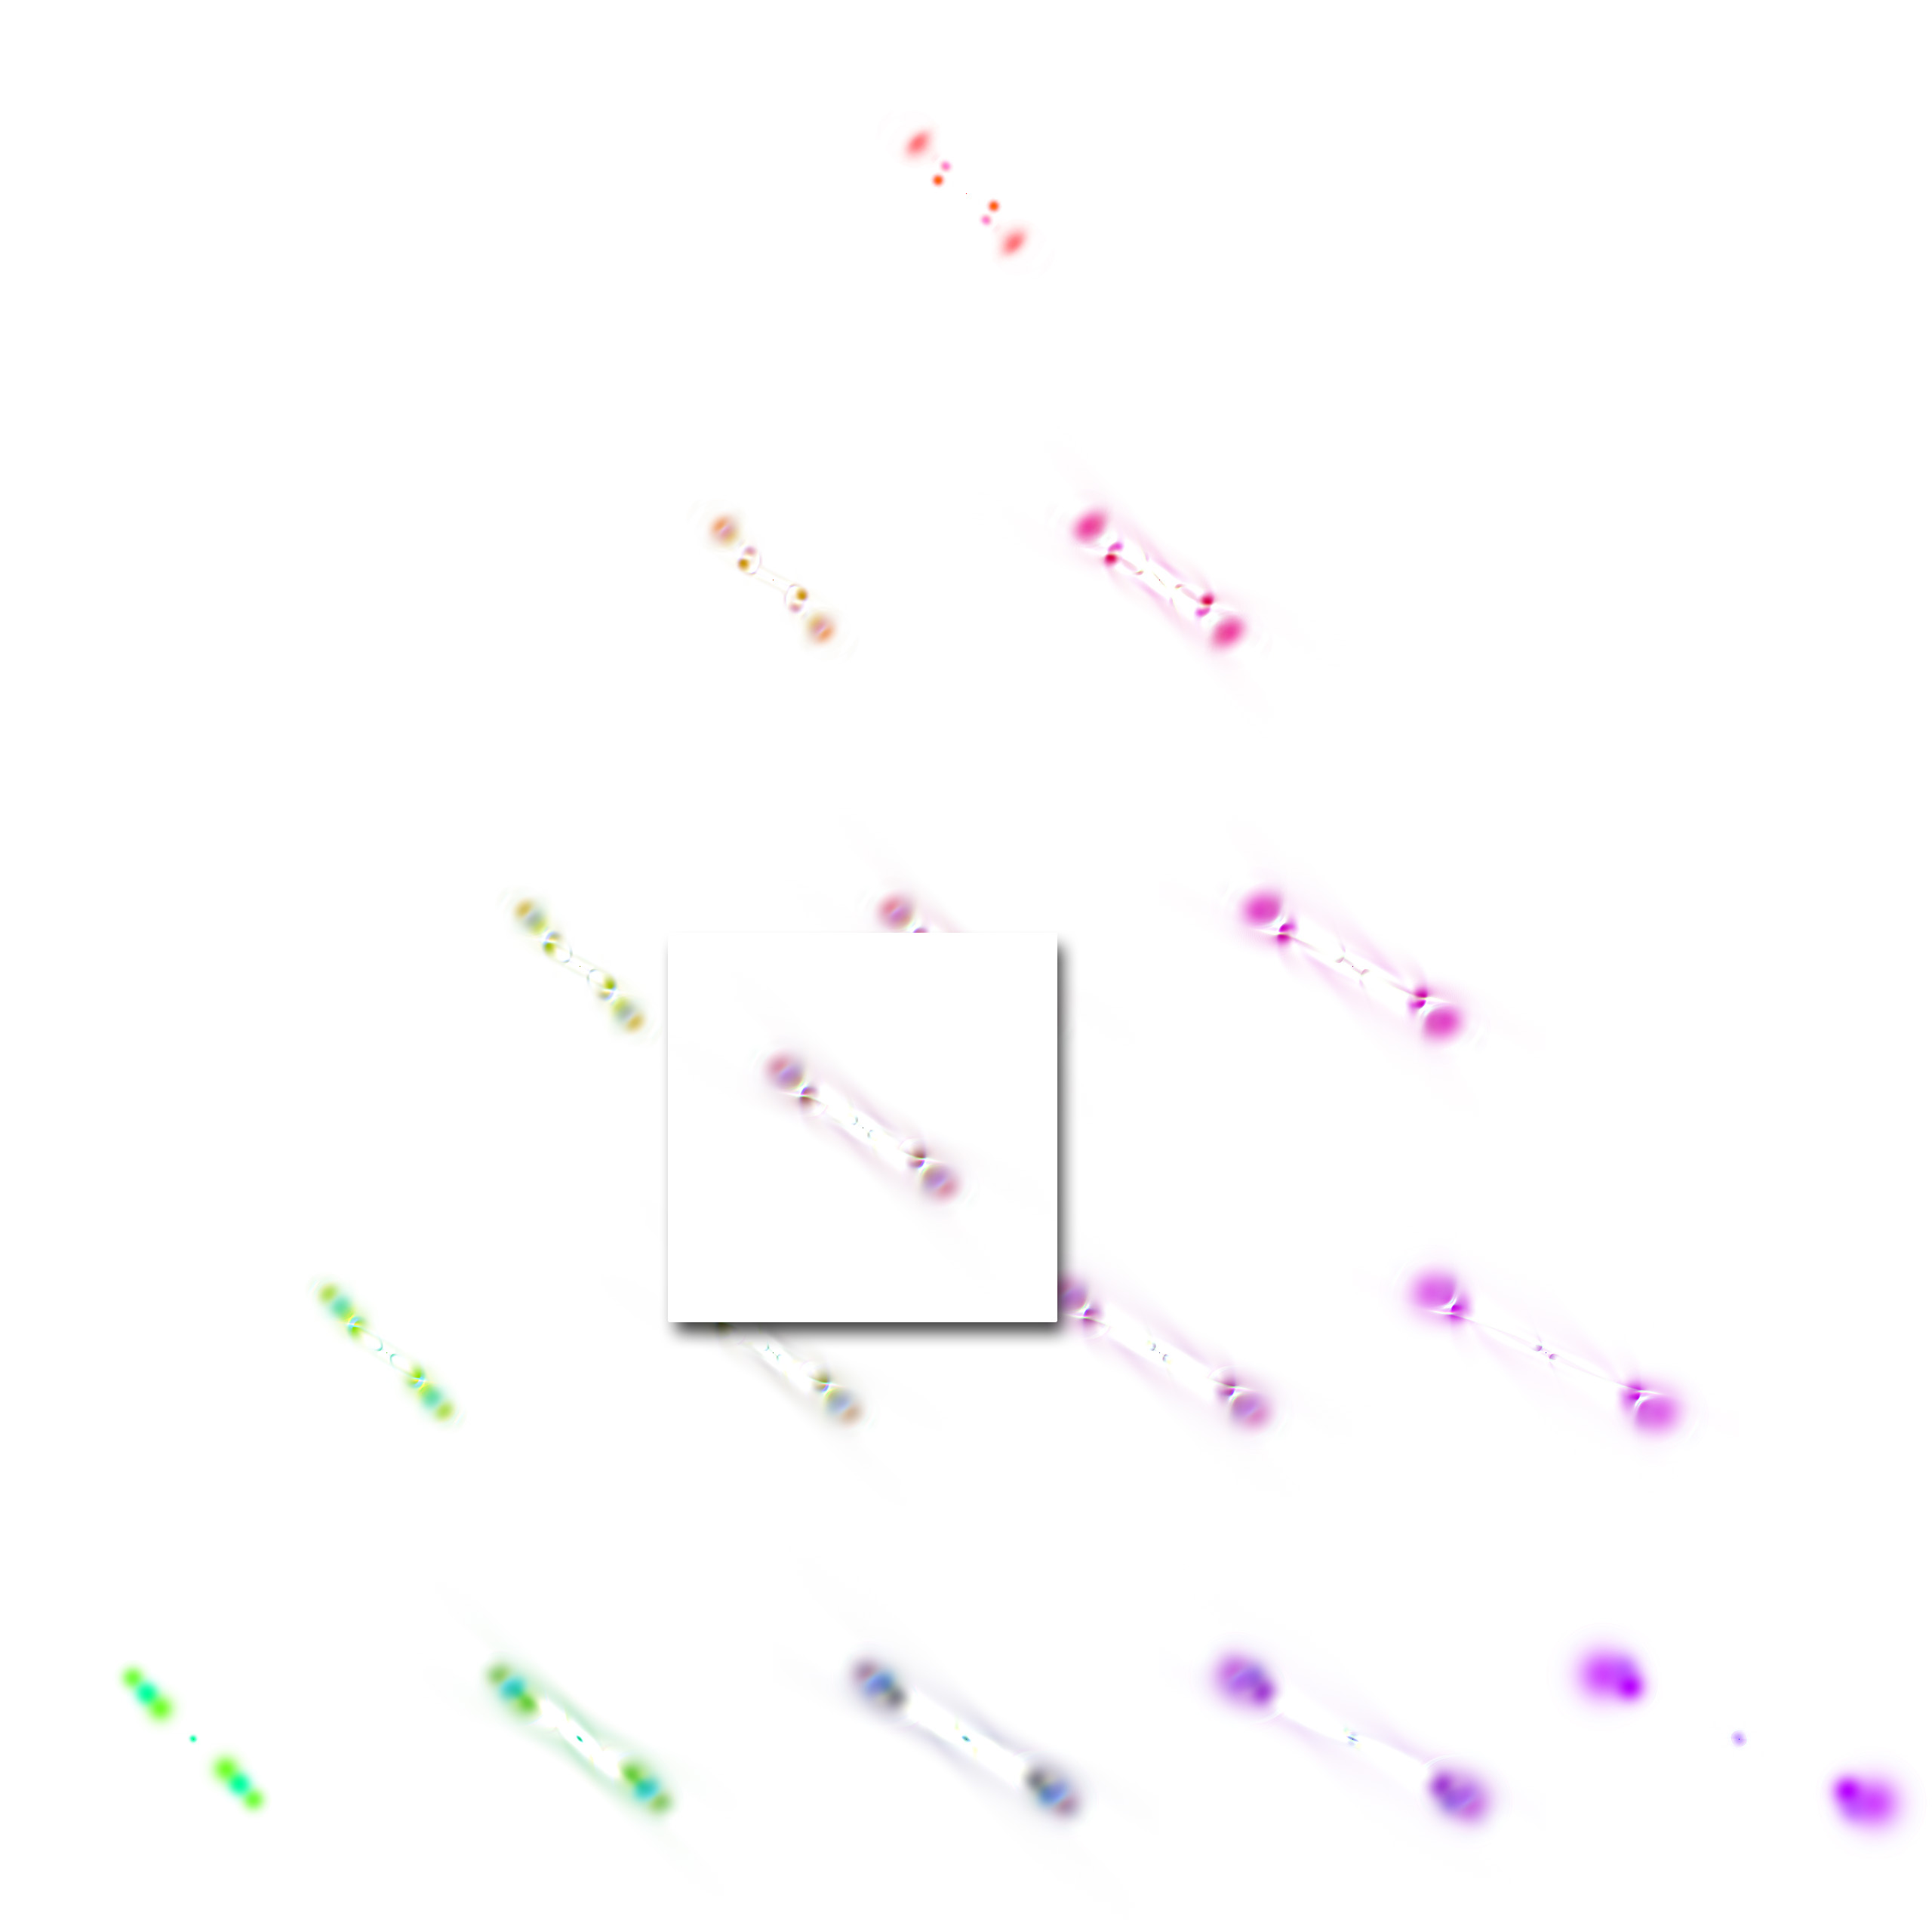
\includegraphics[width=0.3\linewidth]{textures/manCspec_fastslant} &
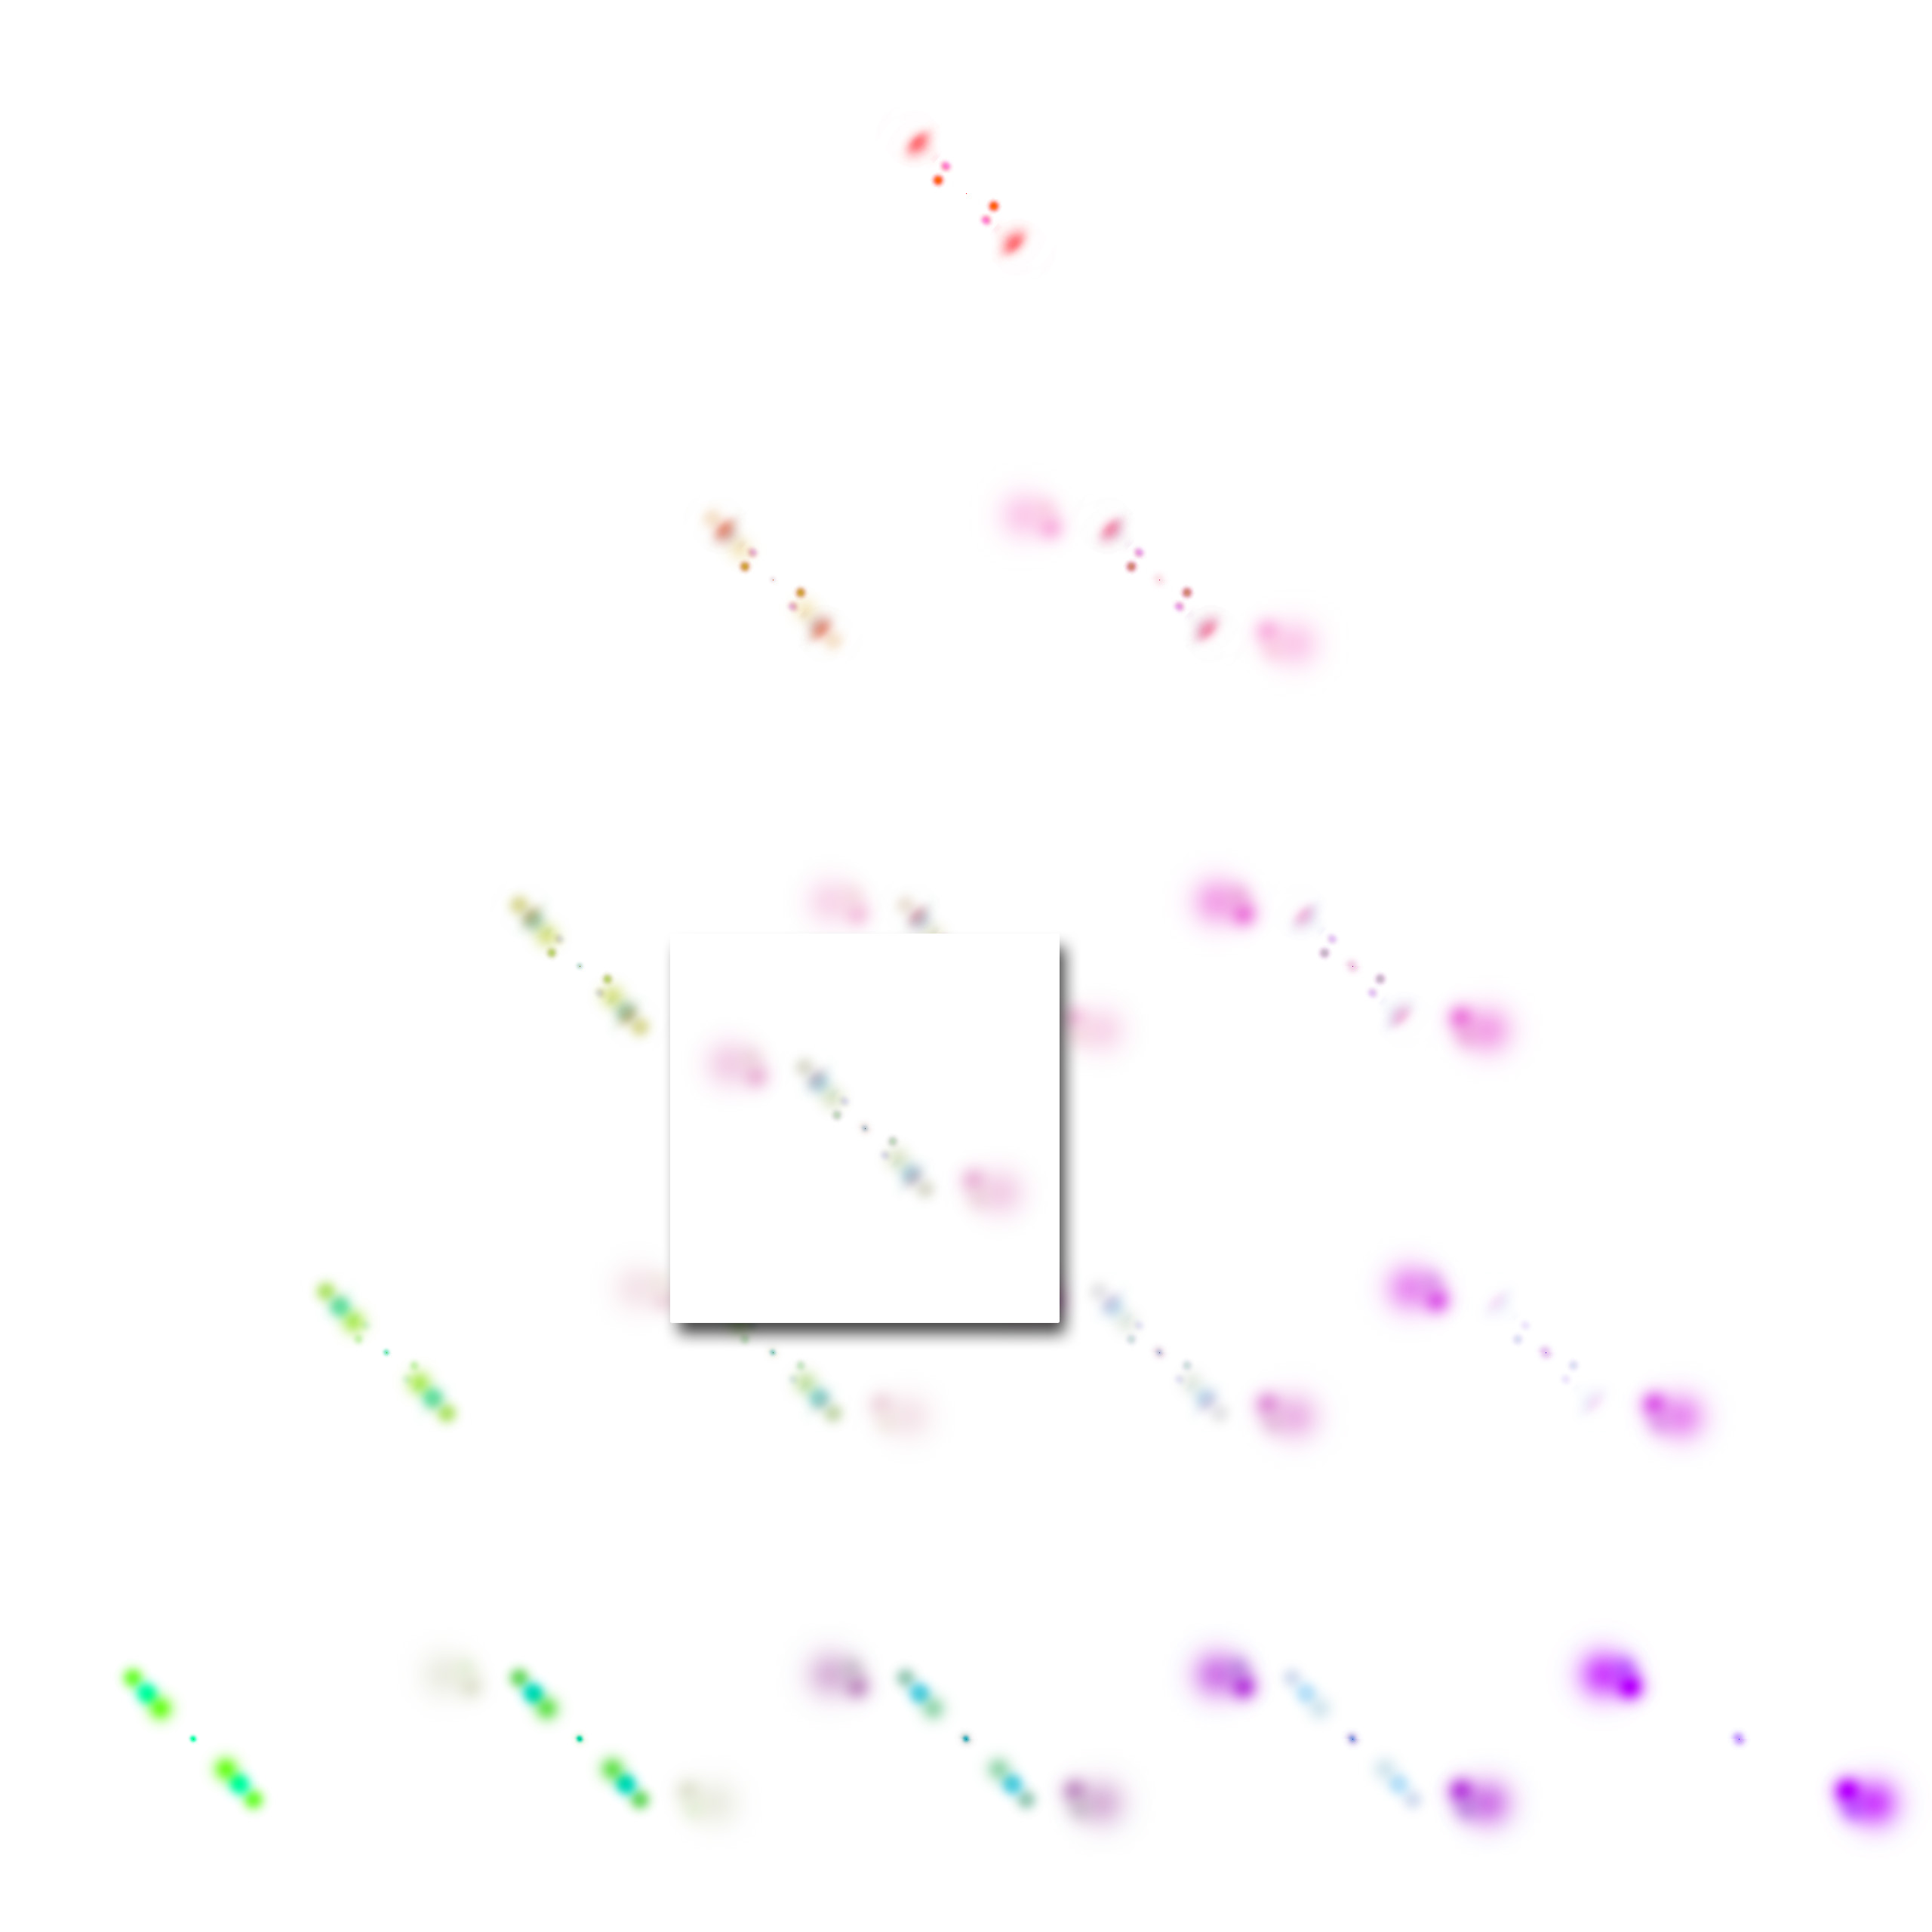
\includegraphics[width=0.3\linewidth]{textures/manCspec_Naive}  \\
 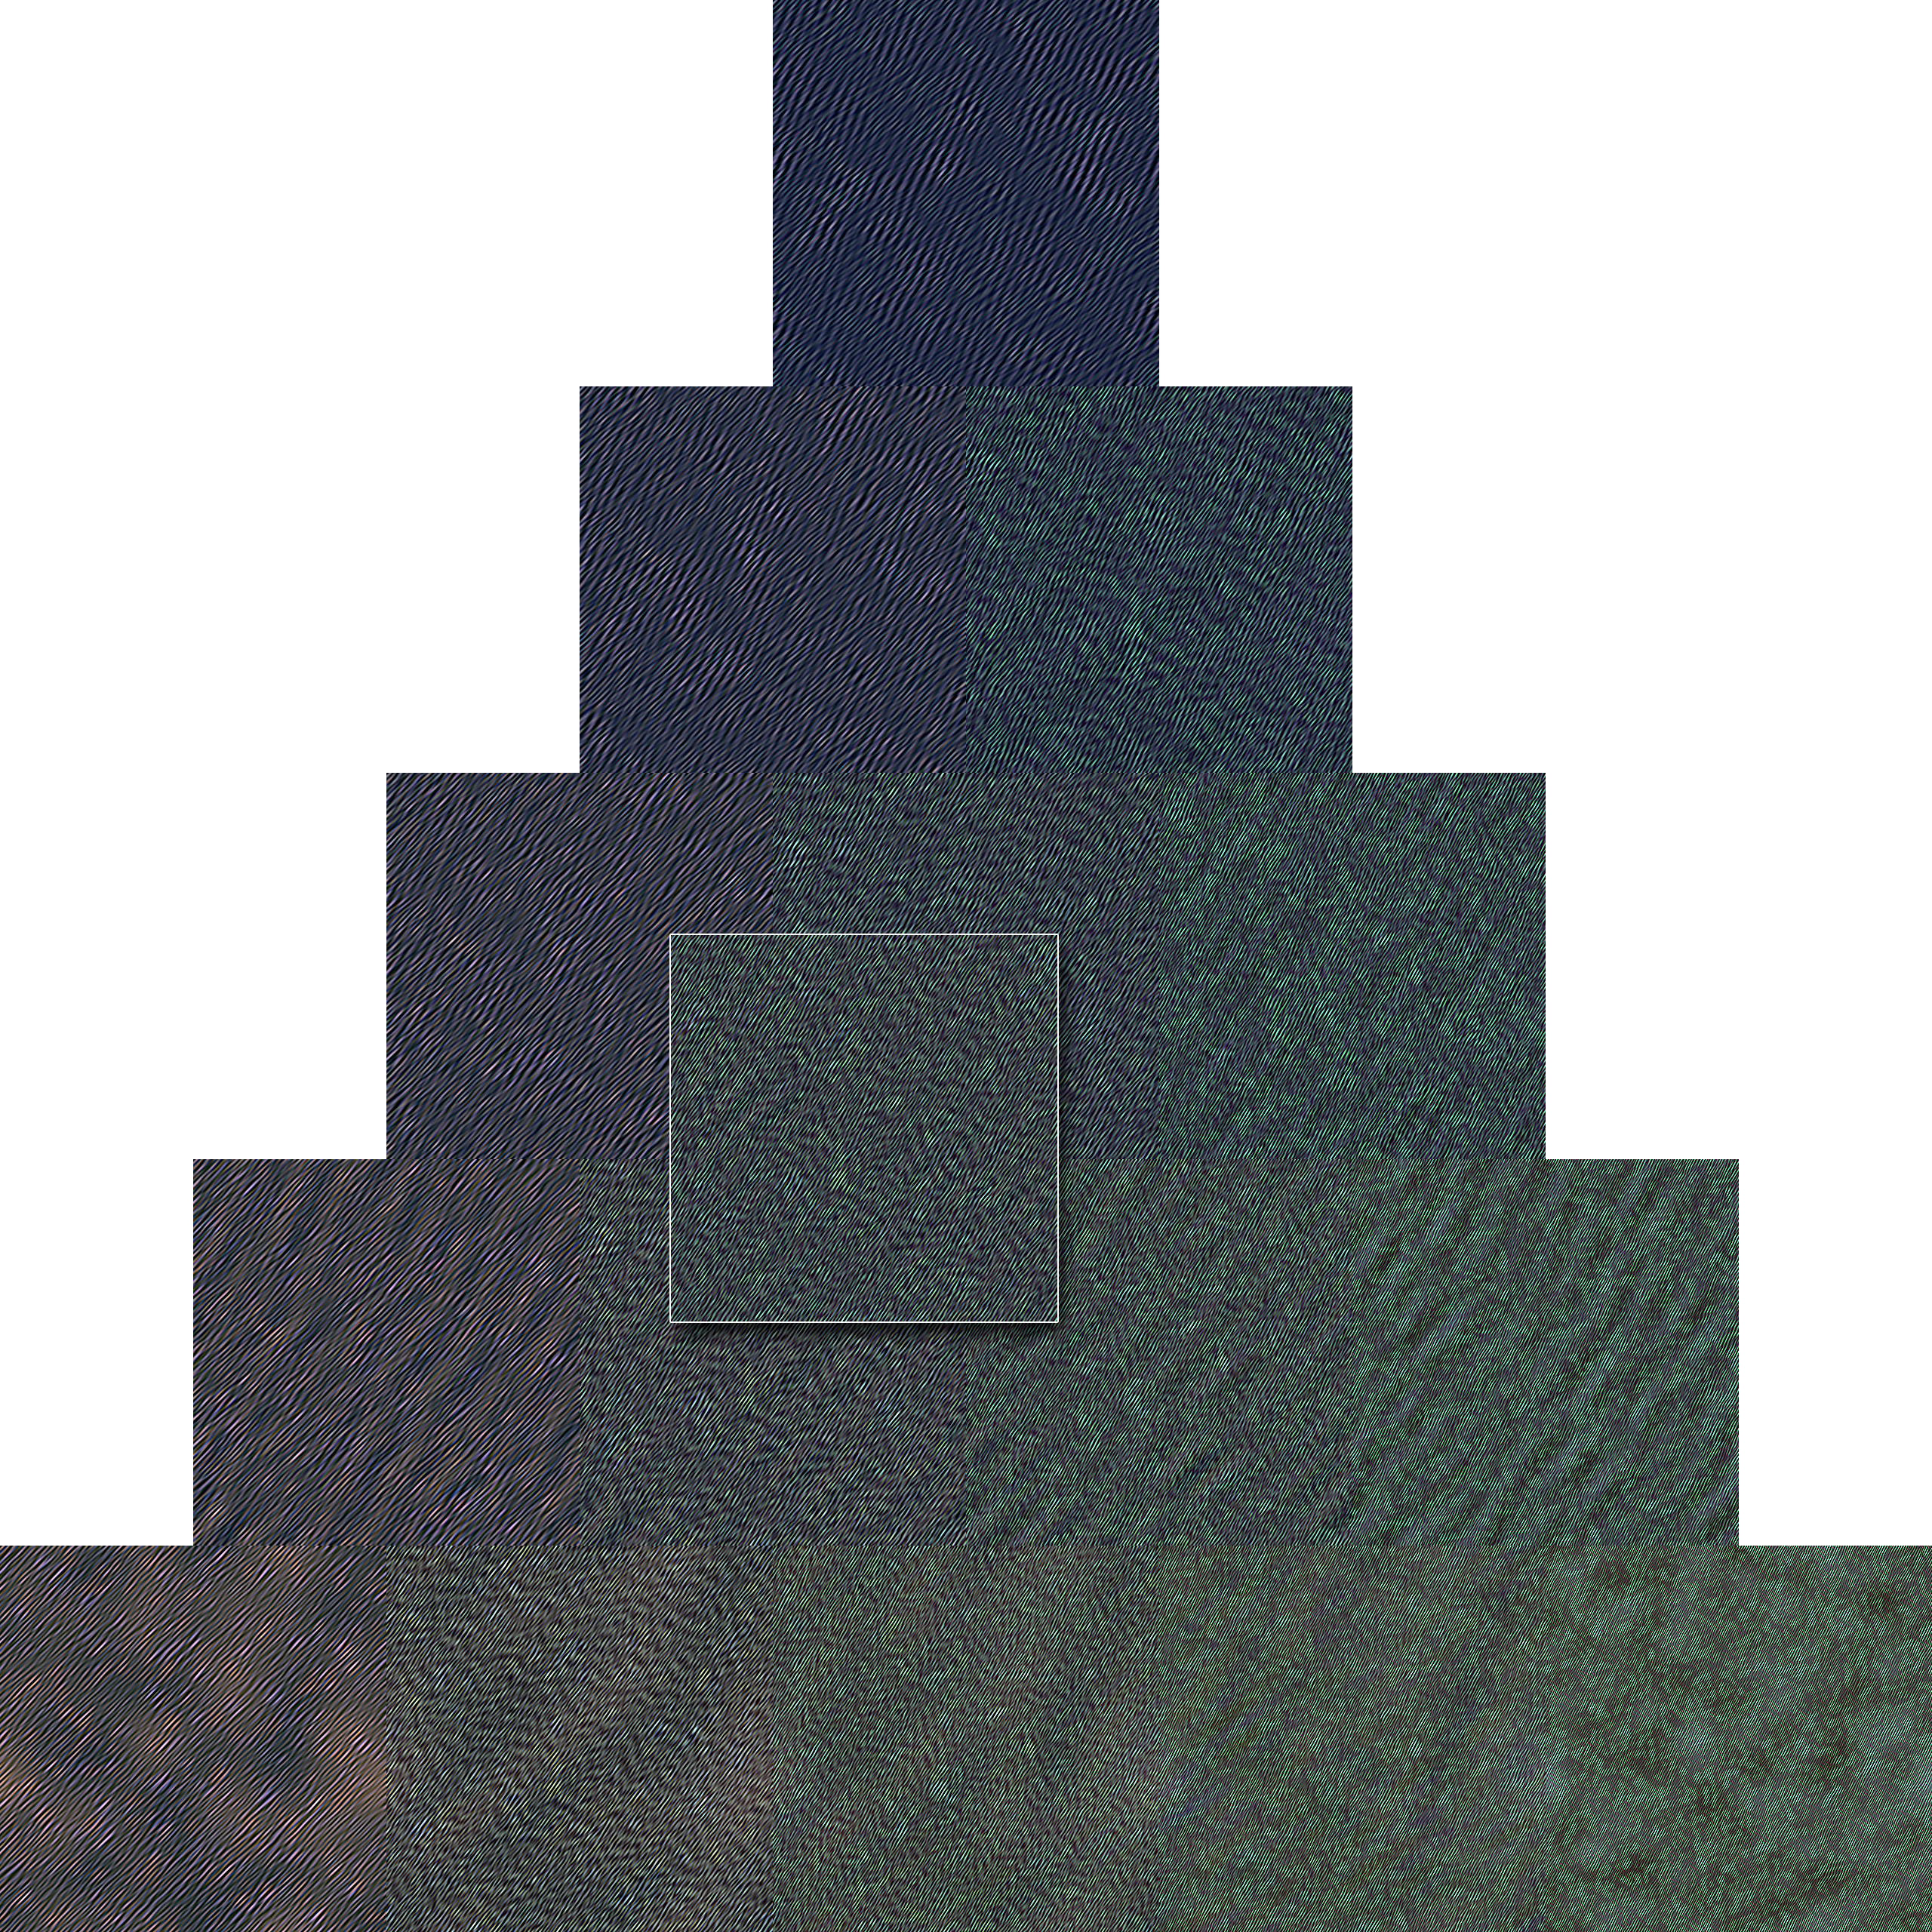
\includegraphics[width=0.49\linewidth]{textures/manC_fastslant}  &
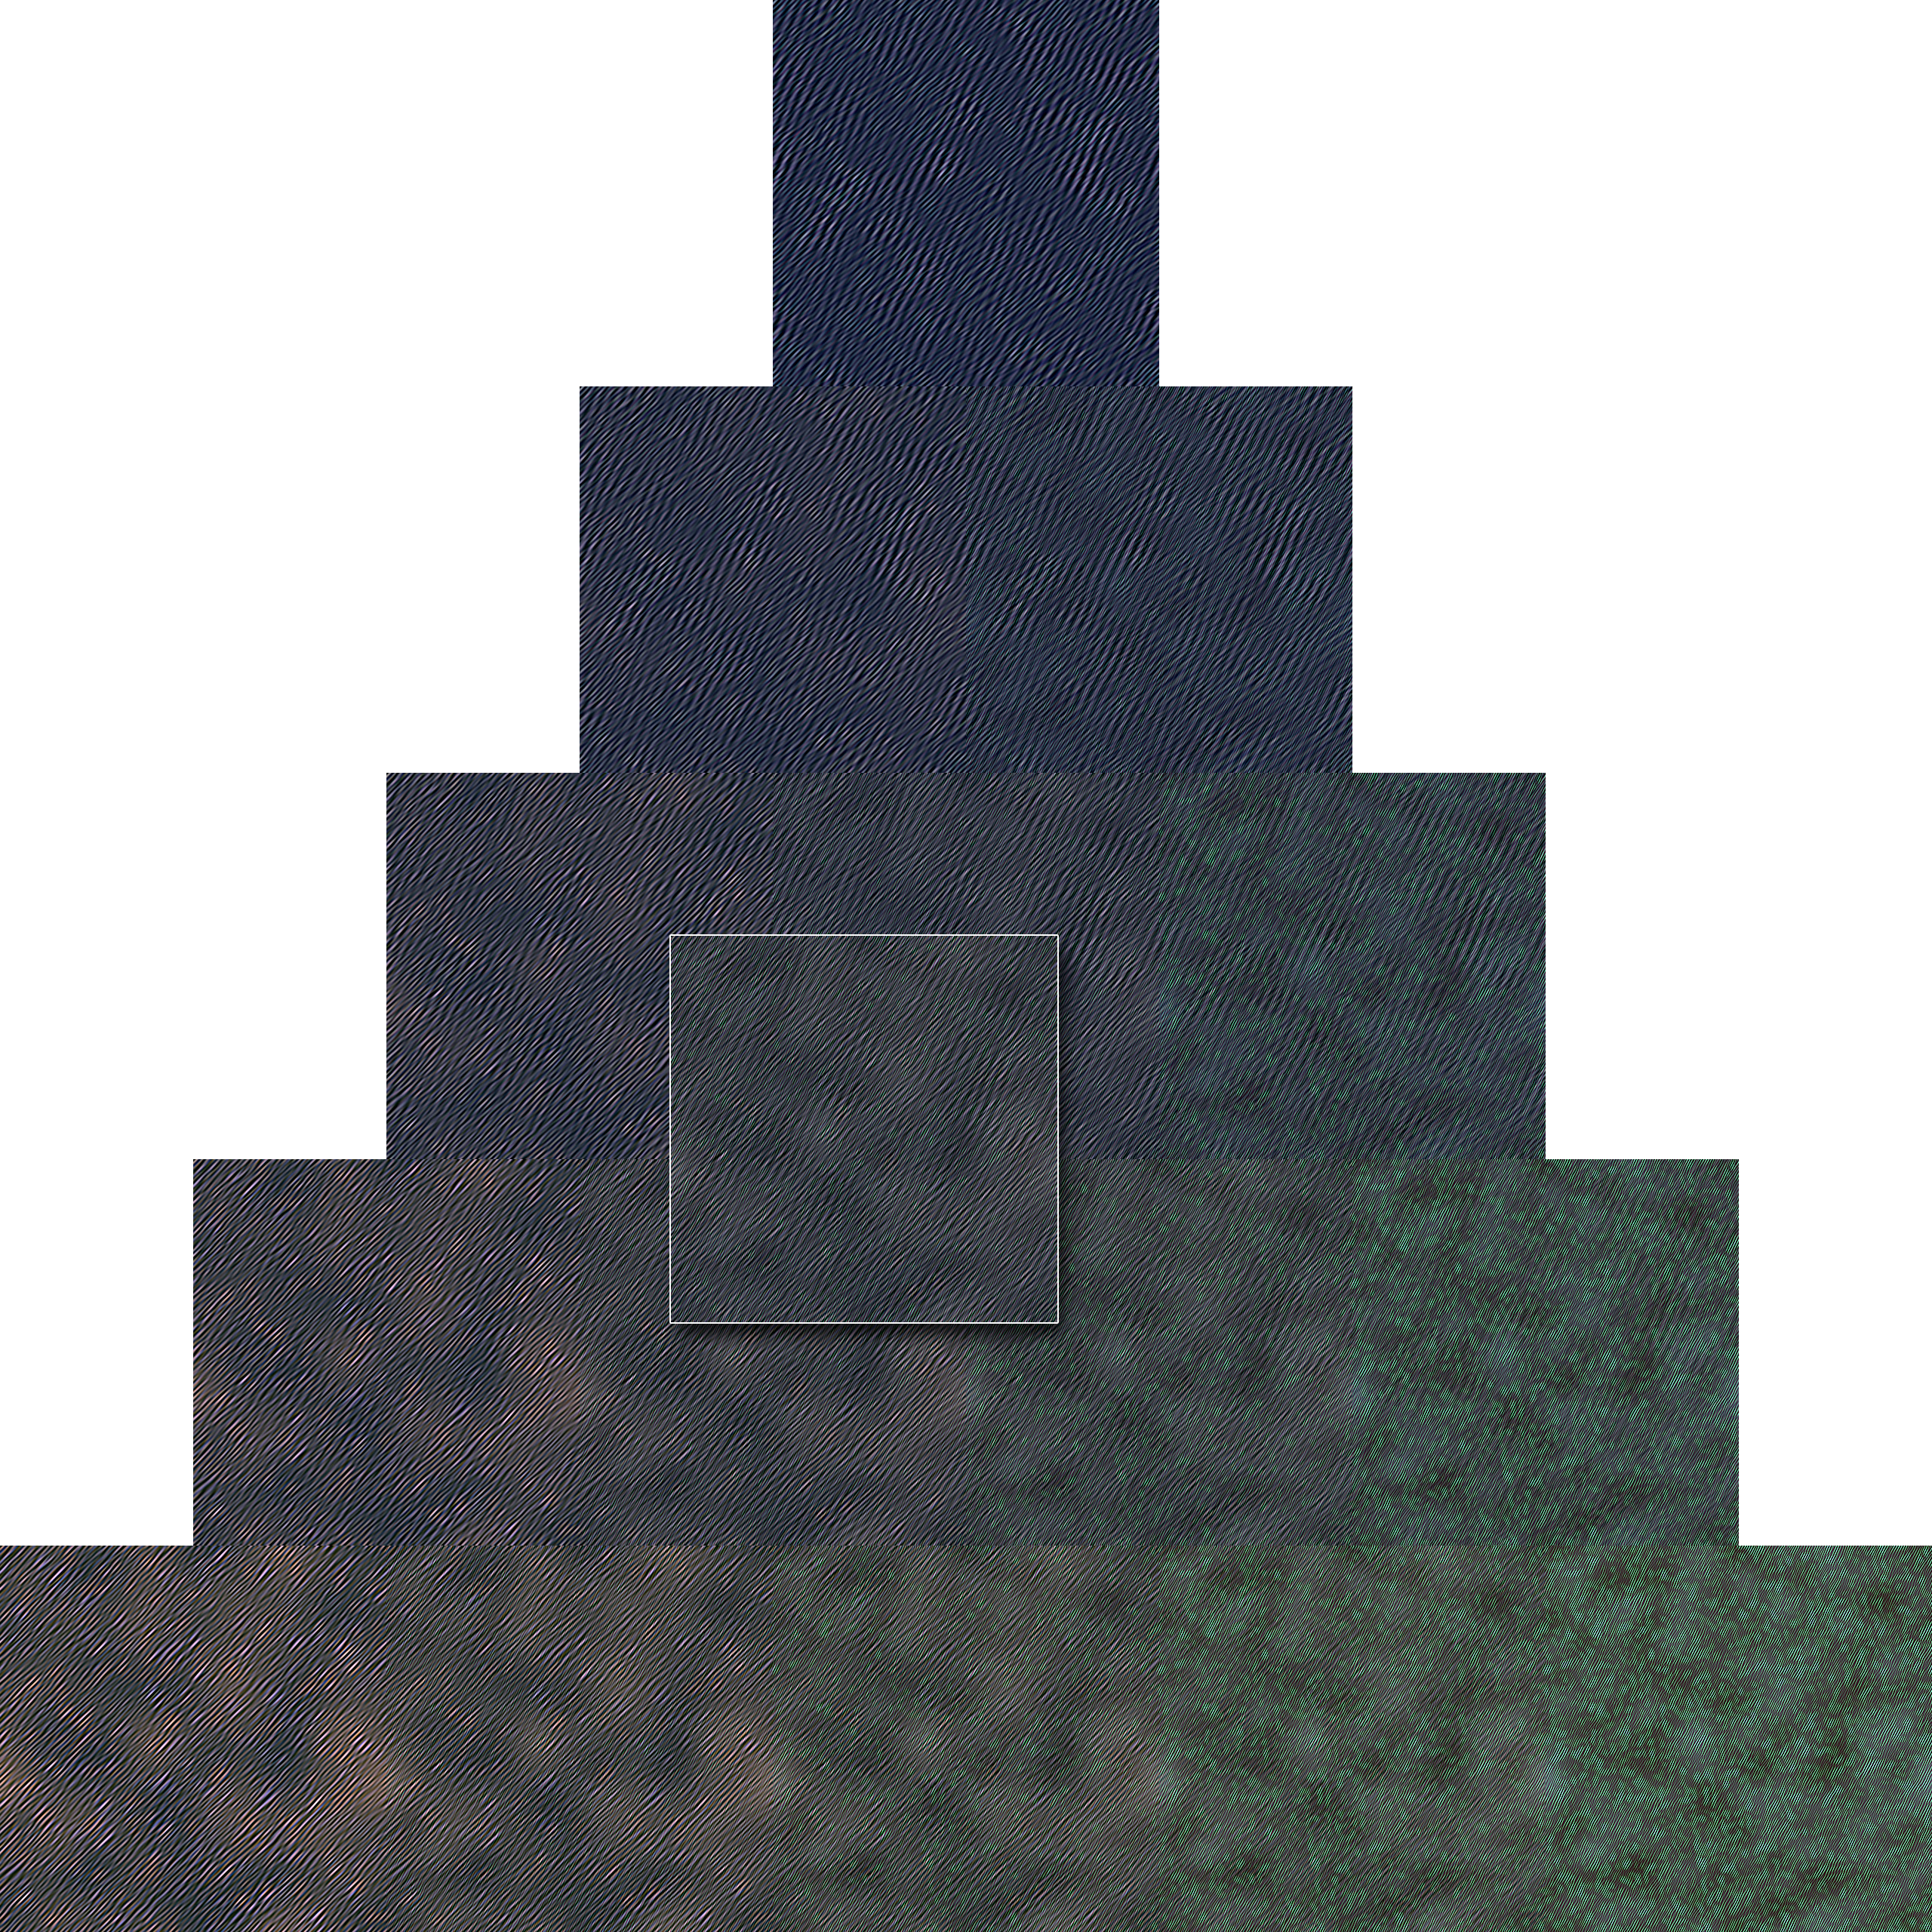
\includegraphics[width=0.49\linewidth]{textures/manC_Naive} \\
(a) Radon barycenter (our approach) & (b) Linear interpolation \protect{\cite{peyre2013Gaussians}}
\end{tabular}
\end{center}
\caption{(a) Eulerian Radon barycenter interpolates sparse amplitude spectra. (b) linear interpolation of the amplitude spectrum~\eqref{eq-interp-linear-spectrum}, as performed in \protect{\cite{peyre2013Gaussians}}. The top row shows the interpolated spectra $P_{F_\la}$.  }
\label{fig:texsynth}
\end{figure*}

\begin{figure*}[!t]
\setlength{\tabcolsep}{0pt}
  \setlength{\fboxsep}{0pt}
\begin{center} 
\begin{tabular}{ccc}
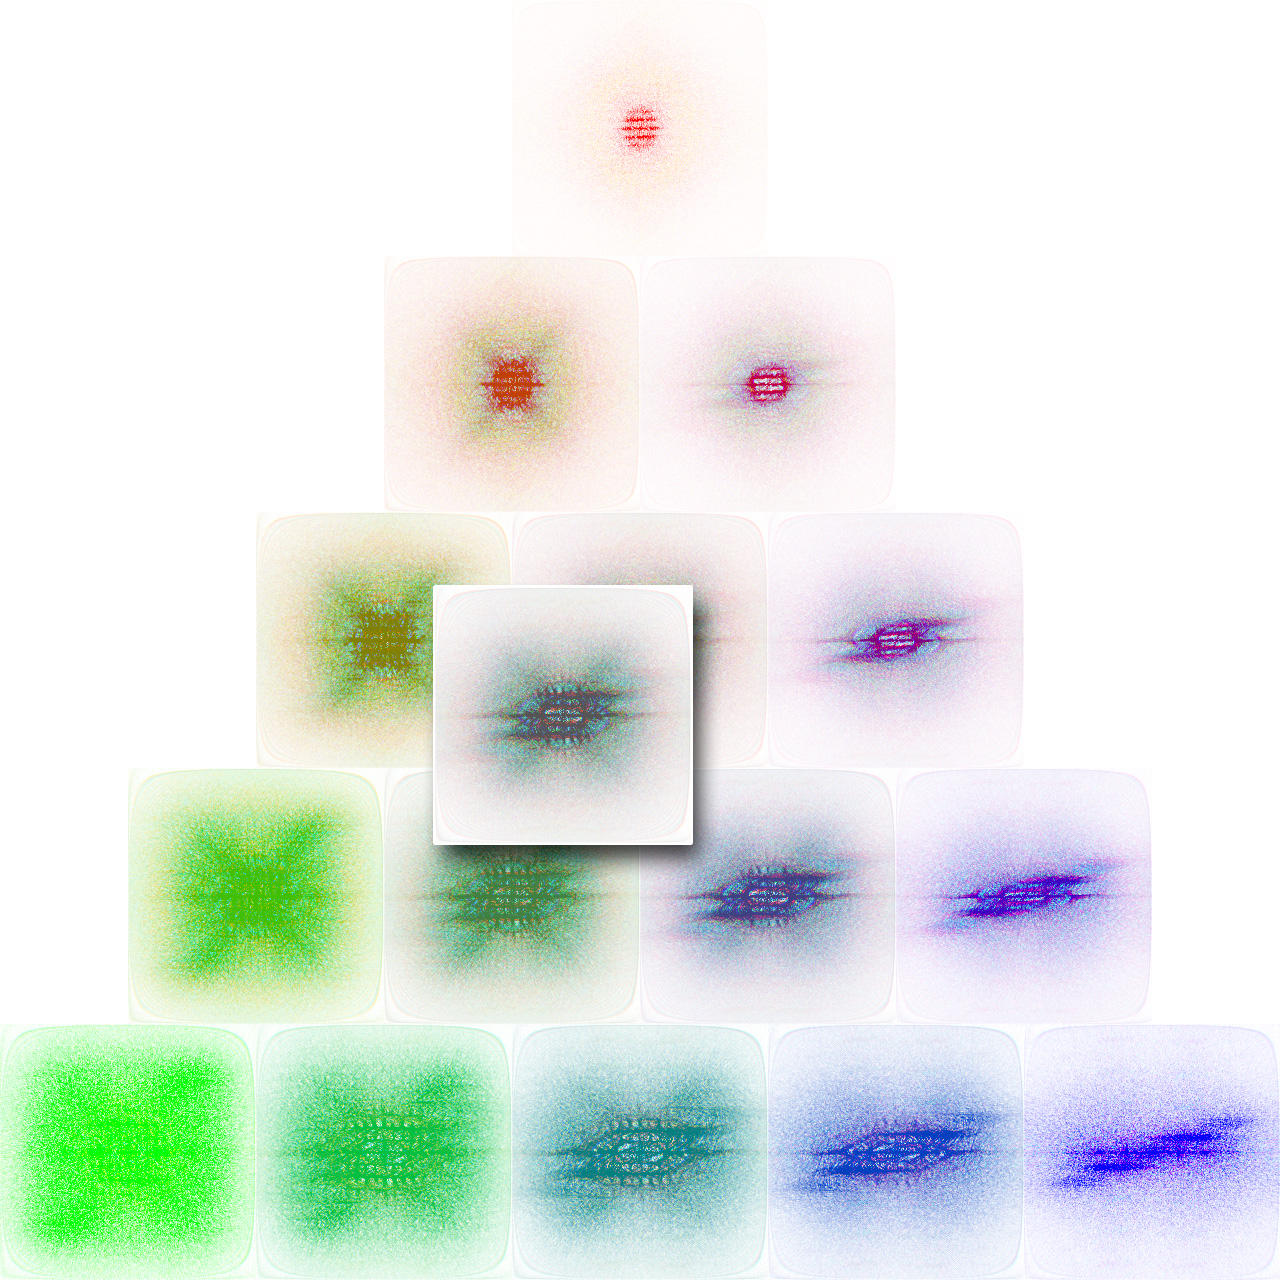
\includegraphics[width=0.48\linewidth]{textures/tex1spec_fastslant} &
 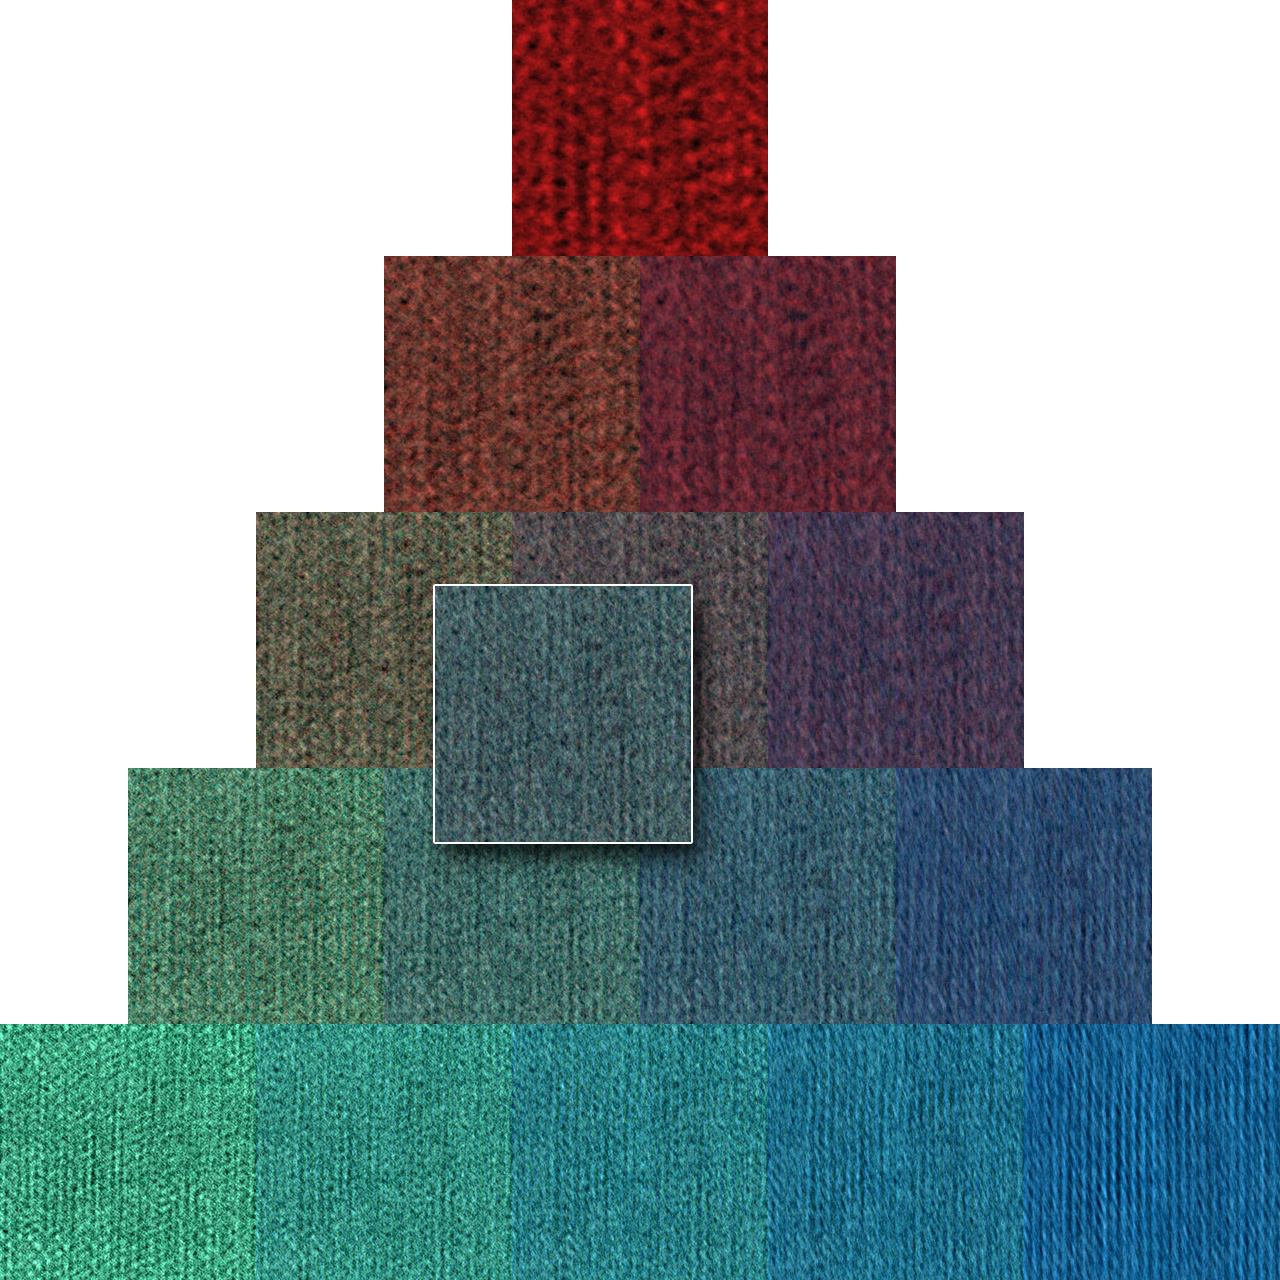
\includegraphics[width=0.48\linewidth]{textures/tex1fastslant} 
\end{tabular}
\end{center}
\caption{Eulerian Radon barycenter applied to the mixing of natural textures.}
\label{fig:texsynth2}
\end{figure*}

%%%%%
\paragraph{Comparison with linear interpolation.}

In~\cite{peyre2013Gaussians}, the authors also use optimal transport to perform SN model interpolation. Their approach is however radically different since they compute optimal transport geodesics in the space of Gaussian distributions in $\RR^N$, which has a closed form solution. In contrast, we propose to compute the transportation of PSD in $\RR^2$, viewed as discrete distributions of $N$ Diracs. For grayscale textures, the method detailed in~\cite{peyre2013Gaussians} thus boils down to a linear interpolation of the PSD, i.e., they define the PSD of the barycentric model $\tilde F_\la$ as
\eql{\label{eq-interp-linear-spectrum}
	\foralls \la \in \La_I, \quad
	P_{\tilde F_\la} = \sum_{i \in I} \la_i P_{F^{[i]}}.
} 
The effect achieved by our Radon barycenter differs from~\cite{peyre2013Gaussians}. As shown in Figure~\ref{fig:texsynth} and~\ref{fig:texsynth2}, we believe our method is geometrically more meaningful when dealing with textures that have a sparse Fourier expansion, while \cite{peyre2013Gaussians} deal with denser spectra more appropriately. Sparse spectra can occur, for instance, for textures with approximately periodic tiling of repetitive patterns. 



%%%%%%%%%%%%%%%%%%%%%%%%%%%%%%%%%%%%%%%%%%%%%%%%%%%
\subsection{Application to Color Palette Manipulation}
\label{sec-appli-colorization}

In this section we investigate the benefit of our Sliced Wasserstein barycenter for two applications: harmonizing colors in an image sequence, and grading colors of a single image. Color harmonization is the process of bringing the colors of input images to an average color distribution such that the images end up looking more similar. This has several applications such as, for instance, image stitching or enforcing temporal coherence of colors in movies. The second application allows for the editing of a single image by bringing its colors closer to a set of photographs exhibiting particular color palettes. This process is called color grading, and finds applications in photograph enhancement.


% In both cases, the method is a two step process. First, a color palette (i.e., color distribution) is computed using our barycenter. Then, the new color distribution is transferred to each input images using (approximate) optimal transport.

%\todo{I think it is simpler to avoid confusing the reader to make the method a two steps algorithm : first harmonization, then color transfer. } %Nico: I'm not sure what you mean here: is the above ok?

%%
\paragraph{Lagrangian color palette.}

We consider a color image represented as a vector $X \in \RR^{N \times 3}$ of $N$ pixels, so that $X = (X_k)_{k=1,\ldots,N}$ where each pixel $X_k \in \RR^3$ stores the value of a pixel indexed by $k$. 
In the following, we use the YCbCr color space because of its ability to decorrelate color channels, although other color spaces may be used (e.g., the CIE-Lab advocated in~\cite{Reinhard:2011}). 
The color distribution of this image is a measure $\mu_X$ defined in $\RR^3$, and describes the color palette.  We naturally represent this color distribution using a Lagrangian discretization, as defined in~\eqref{eq-lagrangian-discr}, by essentially storing pixel colors as a point cloud in the space of colors. Note that the Lagrangian discretization~\eqref{eq-lagrangian-discr} defining $\mu_X$ is automatically normalized so that $\mu_X \in \Mm_1^+(\RR^2)$. We hence compute the average distribution of multiple images distributions using our (Lagrangian) Sliced Wasserstein Barycenter detailed in Section~\ref{subsec-algorithm-lagrangian}.  

% The color point-cloud of the image $u$ is then obtained as $X_u = \left\{ (Tu)_k \right\}_{k\in M\times N} \in \R^{d\times MN}$, defining the color measure $\mu_u$ as a discrete sum of Dirac masses located in $(Tu)_k$, corresponding to the pixel $Tu(m,n)$ at location $k = m + (n-1)M$.

%%
\paragraph{Color palette transfer.}

Before detailing our main application to color palette barycenters, we illustrate our stochastic gradient descent (Section~\ref{subsec-sliced-assignement}). This descent allows for the computation of an approximate Sliced transport map $T^S$ between the color palette $\mu_{\iterInit{X}}$ of an input image $\iterInit{X}$ and the model palette $\mu_Y$ of an image $Y$, where $\iterInit{X},Y \in \RR^{N \times 3}$. The resulting image $X^\star$ is obtained as the limit of the stochastic gradient descent steps~\eqref{eq-stoch-grad-desc} until convergence
\eql{\label{eq-converg-colorization}
	\iter{X} \overset{\iterInd \rightarrow +\infty}{\longrightarrow} X^\star, 
}
as described in~\eqref{eq-lim-xstar}. 

%\paragraph{Comparison with~\cite{pitie2005n}}
We illustrate our technique in Fig.~\ref{fig:colortransfer2}. This process generalizes the algorithm introduced in~\cite{pitie2005n} that uses $|\Th_\iterInd|=3$ orthogonal directions at each step. 
%Figure~\ref{fig:colortransfer2} shows a comparison of the result obtained with $|\Th_\iterInd|=10$ orientations and the method of~\cite{pitie2005n}. To illustrate differences in the choice of orientations, we did not use any regularization, used the same RGB color space, and kept the number of iterations fixed to 20. This shows that using more directions reduces the visual artifacts created by the transport. 
While we make use of an exact Lagrangian method by sorting pixel values, Piti\'{e} et al. discretize histograms and use the cumulative histogram and pseudo-inverse approach (Eqs.~\ref{eq-cumulative-defn} and \ref{eq-cumulative-pseudoinv-defn}). The lower complexity of ~\cite{pitie2005n} comes at the expense of a discretization which can lead to quantization errors and limits convergence. 


% \cmt{
% The main differences of this approach in comparison to ours are:
% \begin{itemize}
% \item it makes use of cumulative histograms \eqref{eq-cumulative-defn} and pseudo-inverse \eqref{eq-cumulative-pseudoinv-defn} to perform 1-D histogram matching iteratively. In practice, this requires a quantization process for computing both histograms and inverse cumulative function, leading to color approximations and quantization error, so that the algorithm does not properly converge. The resulting color histogram is still very close to the target one in practice. % Nico: si on dit que ca ne converge pas de maniere forte, il faut montrer des plots, des tests, etc. On peut faire ca, mais on peut aussi nous dire que "peu importe puisque ca donne de jolis resultats quand meme"... Le but n'est pas non plus de basher Pitie qui va peut etre nous reviewer ;)

% \item the time complexity of this approach is linear $O(q)$ in the number of quantized colors $q$ (observe that the quantization must be performed simultaneously for both input and target color palettes, but also for color quantiles), whereas ours makes use of a sorting algorithm and results therefore in $O\big(N\log(N)\big)$. % Nico: donc notre approche est plus complexe (sauf a utiliser plus de bins que de pixels...!). On va pas insister dessus hein ;)

% \item the basis direction set $\Theta^{[k]}$ to be used at iteration $k$ is precomputed in order to minimize the correlation with previous directions;  % Nico: Je ne pense pas que ca soit important (sinon faut dire pourquoi ca l'est). On pourrait faire pareil par exemple, et on pourrait nous demander pourquoi on fait pas ca.

% \end{itemize}
% }

%\todo{what is smoother? pitie? ours? the wasserstein plan that we both approximate?}.  \todo{Apparently, using more direction leads to a better transport ? Is it correct ? Why ? Some more comments are needed.} \todo{Also note that I directly too Pitie's code ; the regularization might be different etc. I was more intending a qualitative comparison}
%\cmt{Julien : Piti� ne fournit pas le code pour la r�gularisation, mais seulement pour le transfert de couleur, ce qui donne des artefacts.}



% Note that transferring the colors of an image to another can be performed with our stochastic gradient descent, which directly generalizes the method proposed in~\cite{pitie2005n}. The algorithm proposed by Piti\'{e} et al.~\cite{pitie2005n} corresponds to our stochastic gradient descent when the subset of orientations $\Th_\iterInd$ chosen at each iteration is a set of three orthogonal directions drawn uniformly at random. We do not impose this restriction. A color transfer result can be see in Fig.~\ref{fig:colortransfer2}.

\begin{figure}[!t]
%
\begin{center} 
\begin{tabular}{@{}c@{\hspace{2mm}}c@{}}
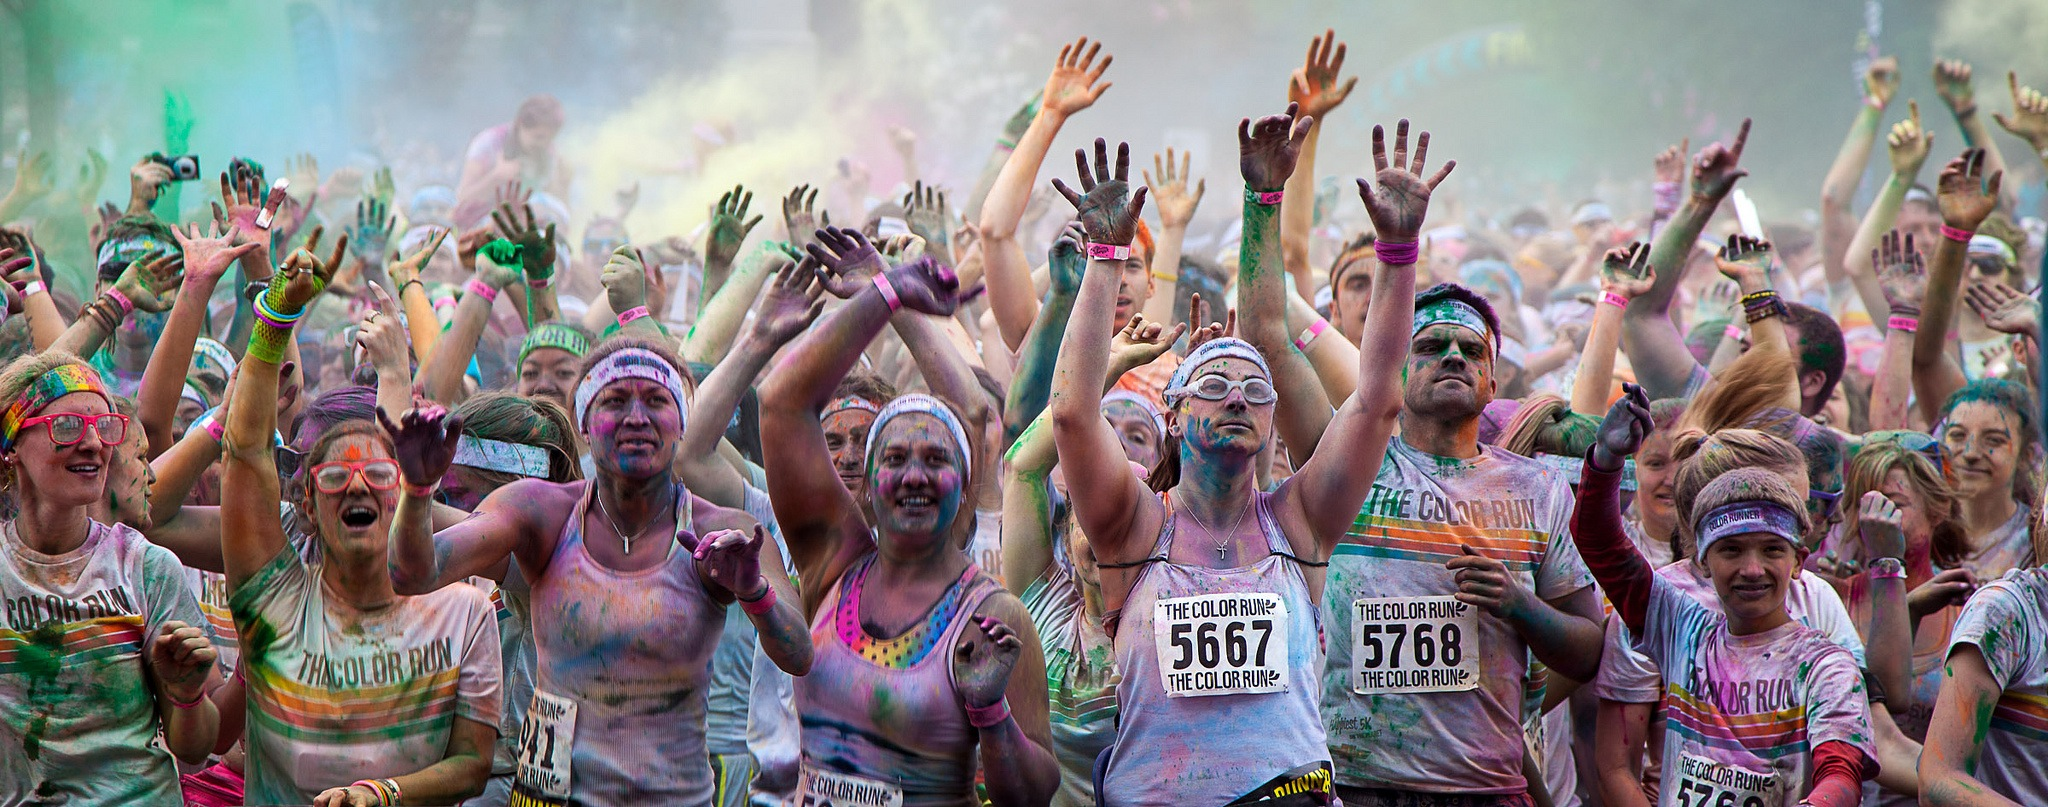
\includegraphics[height=2cm]{color/8733654151_b9422bb2ec_k} &
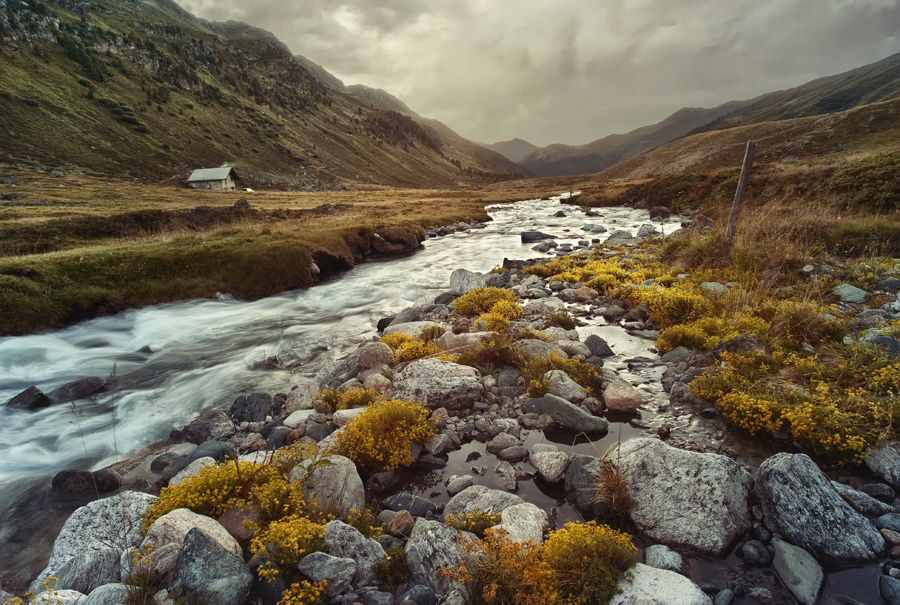
\includegraphics[height=2cm]{color/4852775794_c671f133d0_b} \\
(a) input image $\iterInit{X}$  & (b) input model $Y$ \\
\end{tabular}
\begin{tabular}{@{}c@{}}
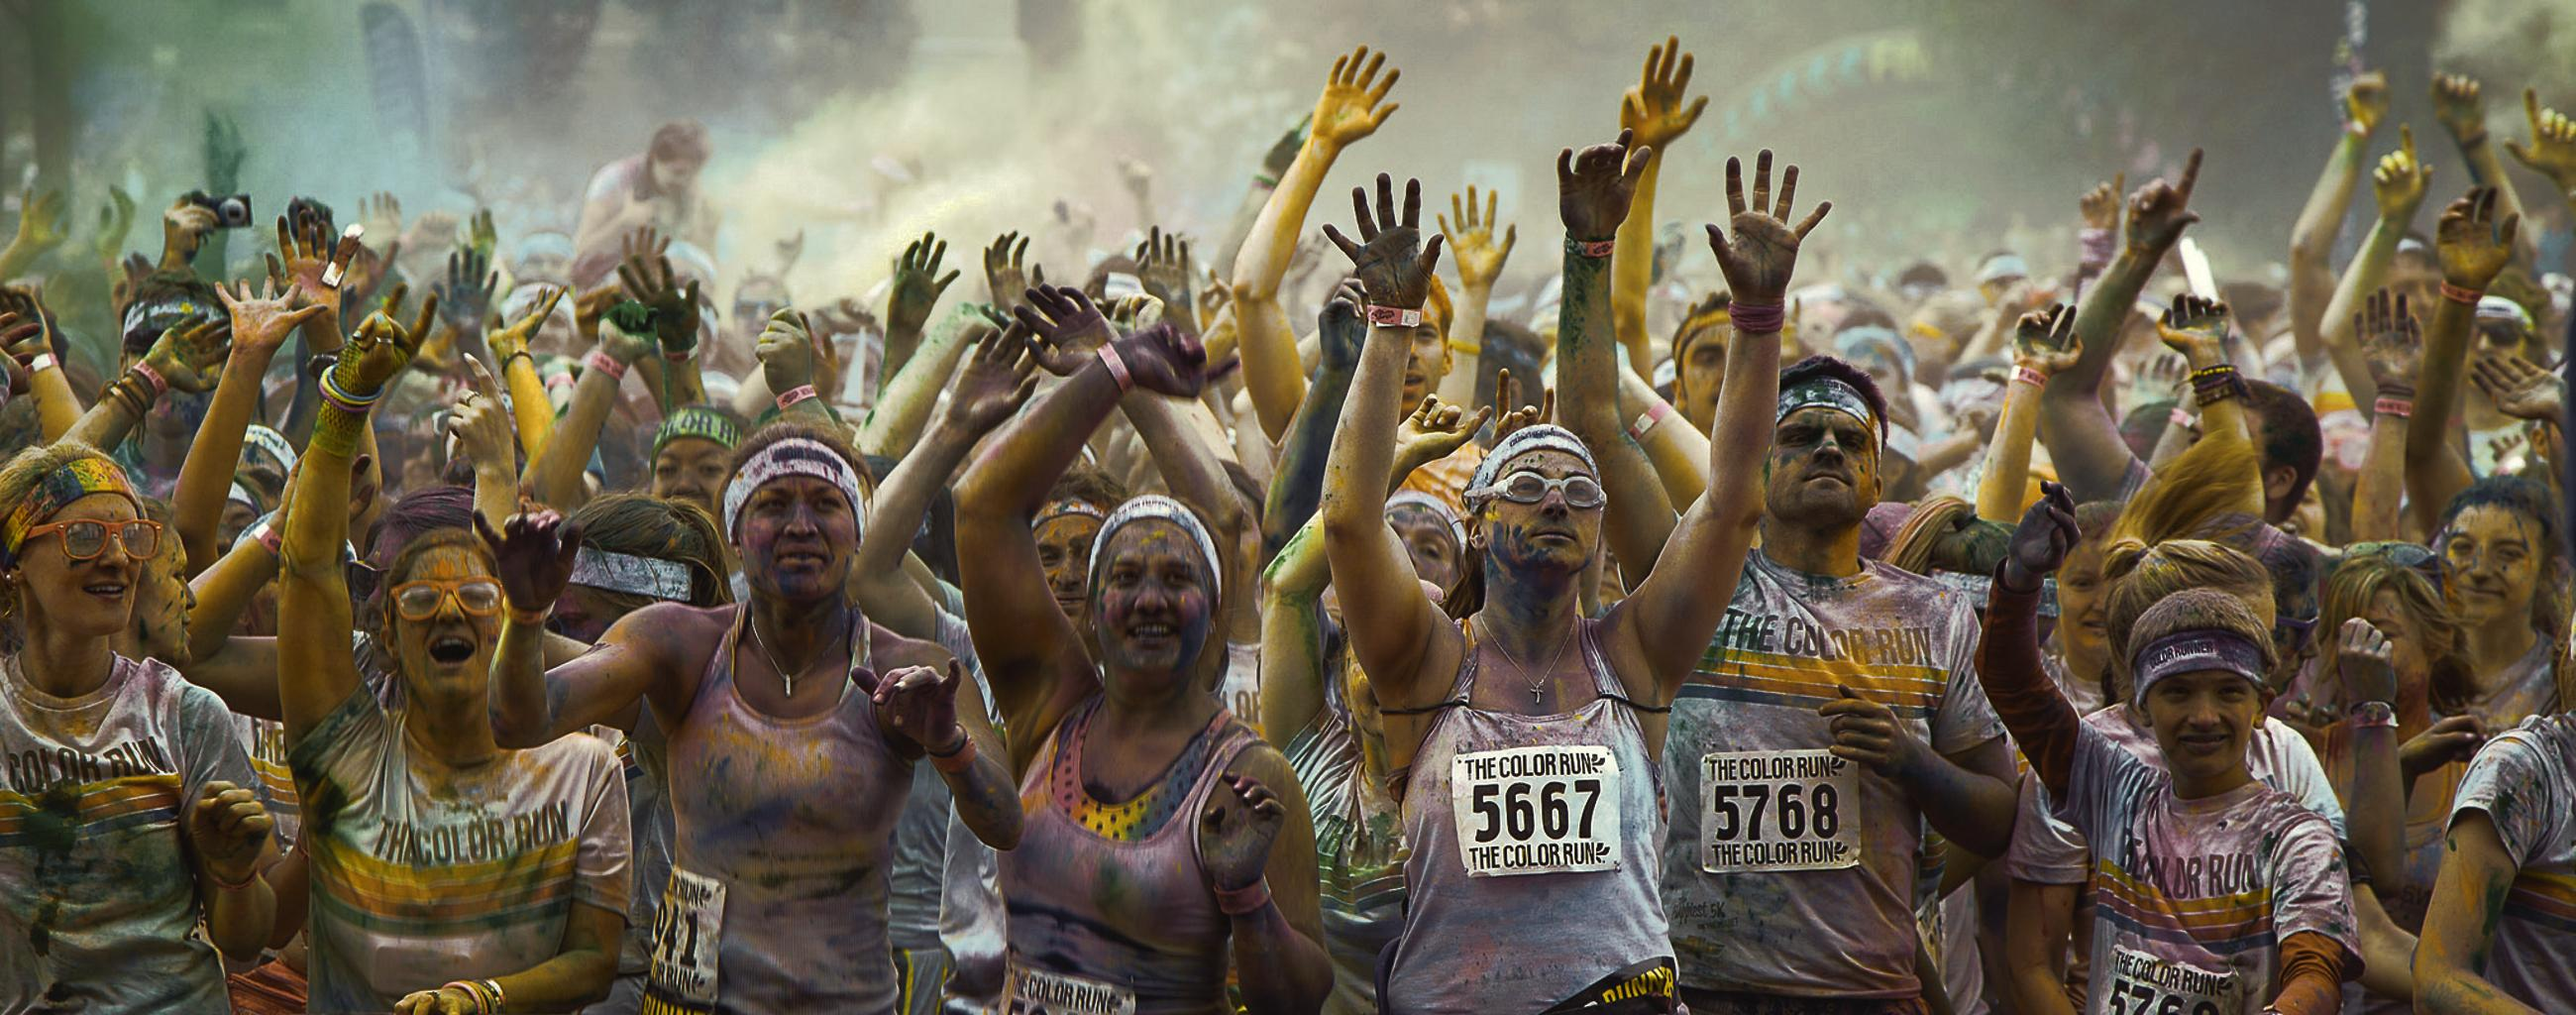
\includegraphics[width=\columnwidth]{color/color_transfer_20iters_noreg_rgb_10dirs}\\ 
(c) our result $X^\star$ 
\end{tabular}
\vspace{-0.2cm}
\end{center} 
%
\caption{Our stochastic gradient descent (c) can be used to transfer the colors of a model image (b) to an input image (a). We generalize the method of Piti\'{e} et al.~\protect{\cite{pitie2005n}} as described in Sec.~\ref{sec-appli-colorization}
%\cmt{Julien : pour �tre ``fair'', il faut que l'on enl�ve la r�gularisation} %ok
}
\label{fig:colortransfer2}
\end{figure}


%%
\paragraph{Color palette barycenter.}

% Let $\{u^{(i)}\}_{i\in I}$ be the color-sequence and 

We consider a set $\{X^{(i)}\}_{i\in I}$ of color images, as well as a particular input color image $\iterInit{X}$. Using~\eqref{eq-non-convx-pointclouds}, we define the color palette $\mu_{X^\star}$, the barycenter of the input palettes $\mu_{X^{(i)}}$, as the Sliced Wasserstein barycenter\\ 
%\eq{
	$\mu_{X^\star} \approx \Bary{\RR^d}^S\pa{ 
			\mu_{X^{(i)}}, \la_i 
		}_{i\in I}$
%}
with weights $\lambda \in \La_I$. 

%%%
\paragraph{Color image harmonization and color grading.}

In order to adjust colors in an image, we are interested in an image $X^\star$ visually similar to $\iterInit{X}$, but whose palette closely matches the palette barycentre $\mu_{X^\star}$. Similarly to the simple color transfer application (see~\eqref{eq-converg-colorization}), we obtain this image by performing the gradient descent iterations~\eqref{eq-grad-desc-sliced} with initialization $\iterInit{X}$, and define $X^\star$ as the limit image $	\iter{X} \overset{\iterInd \rightarrow +\infty}{\longrightarrow} X^\star$.

However, highly non-linear color transformations can create undesirable visual artifacts. We therefore use an iterative post-processing technique introduced in~\cite{Rabin_artefact} to regularize the transportation map $\iterInit{X}_k \mapsto X^\star_k$. We refer the interested reader to~\cite{Rabin_artefact} for further details. 
% We still denote as $X^\star$ the final harmonized imaged obtained after this pre-processing. 

%We use our technique for manipulating colors. 
For color harmonization,  we apply this process successively to each image in an input sequence $\{ X^{(i)} \}_{i \in I}$, by initializing $\iterInit{X}$ with $X^{(i)}$ for each $i$. %We denote our resulting images $X^{(i,\star)} \leftarrow X^\star$.  \cmt{Nico: why would we introduce a notation that we won't use?}
For color grading, we instead apply the palette barycenter to an arbitrary input image $\iterInit{X}$. %, which is, in general, different from any of the input images in $\{ X^{(i)} \}_{i \in I}$. 

\begin{figure*}[!t]
\begin{center} 
\raisebox{-0.5\height}{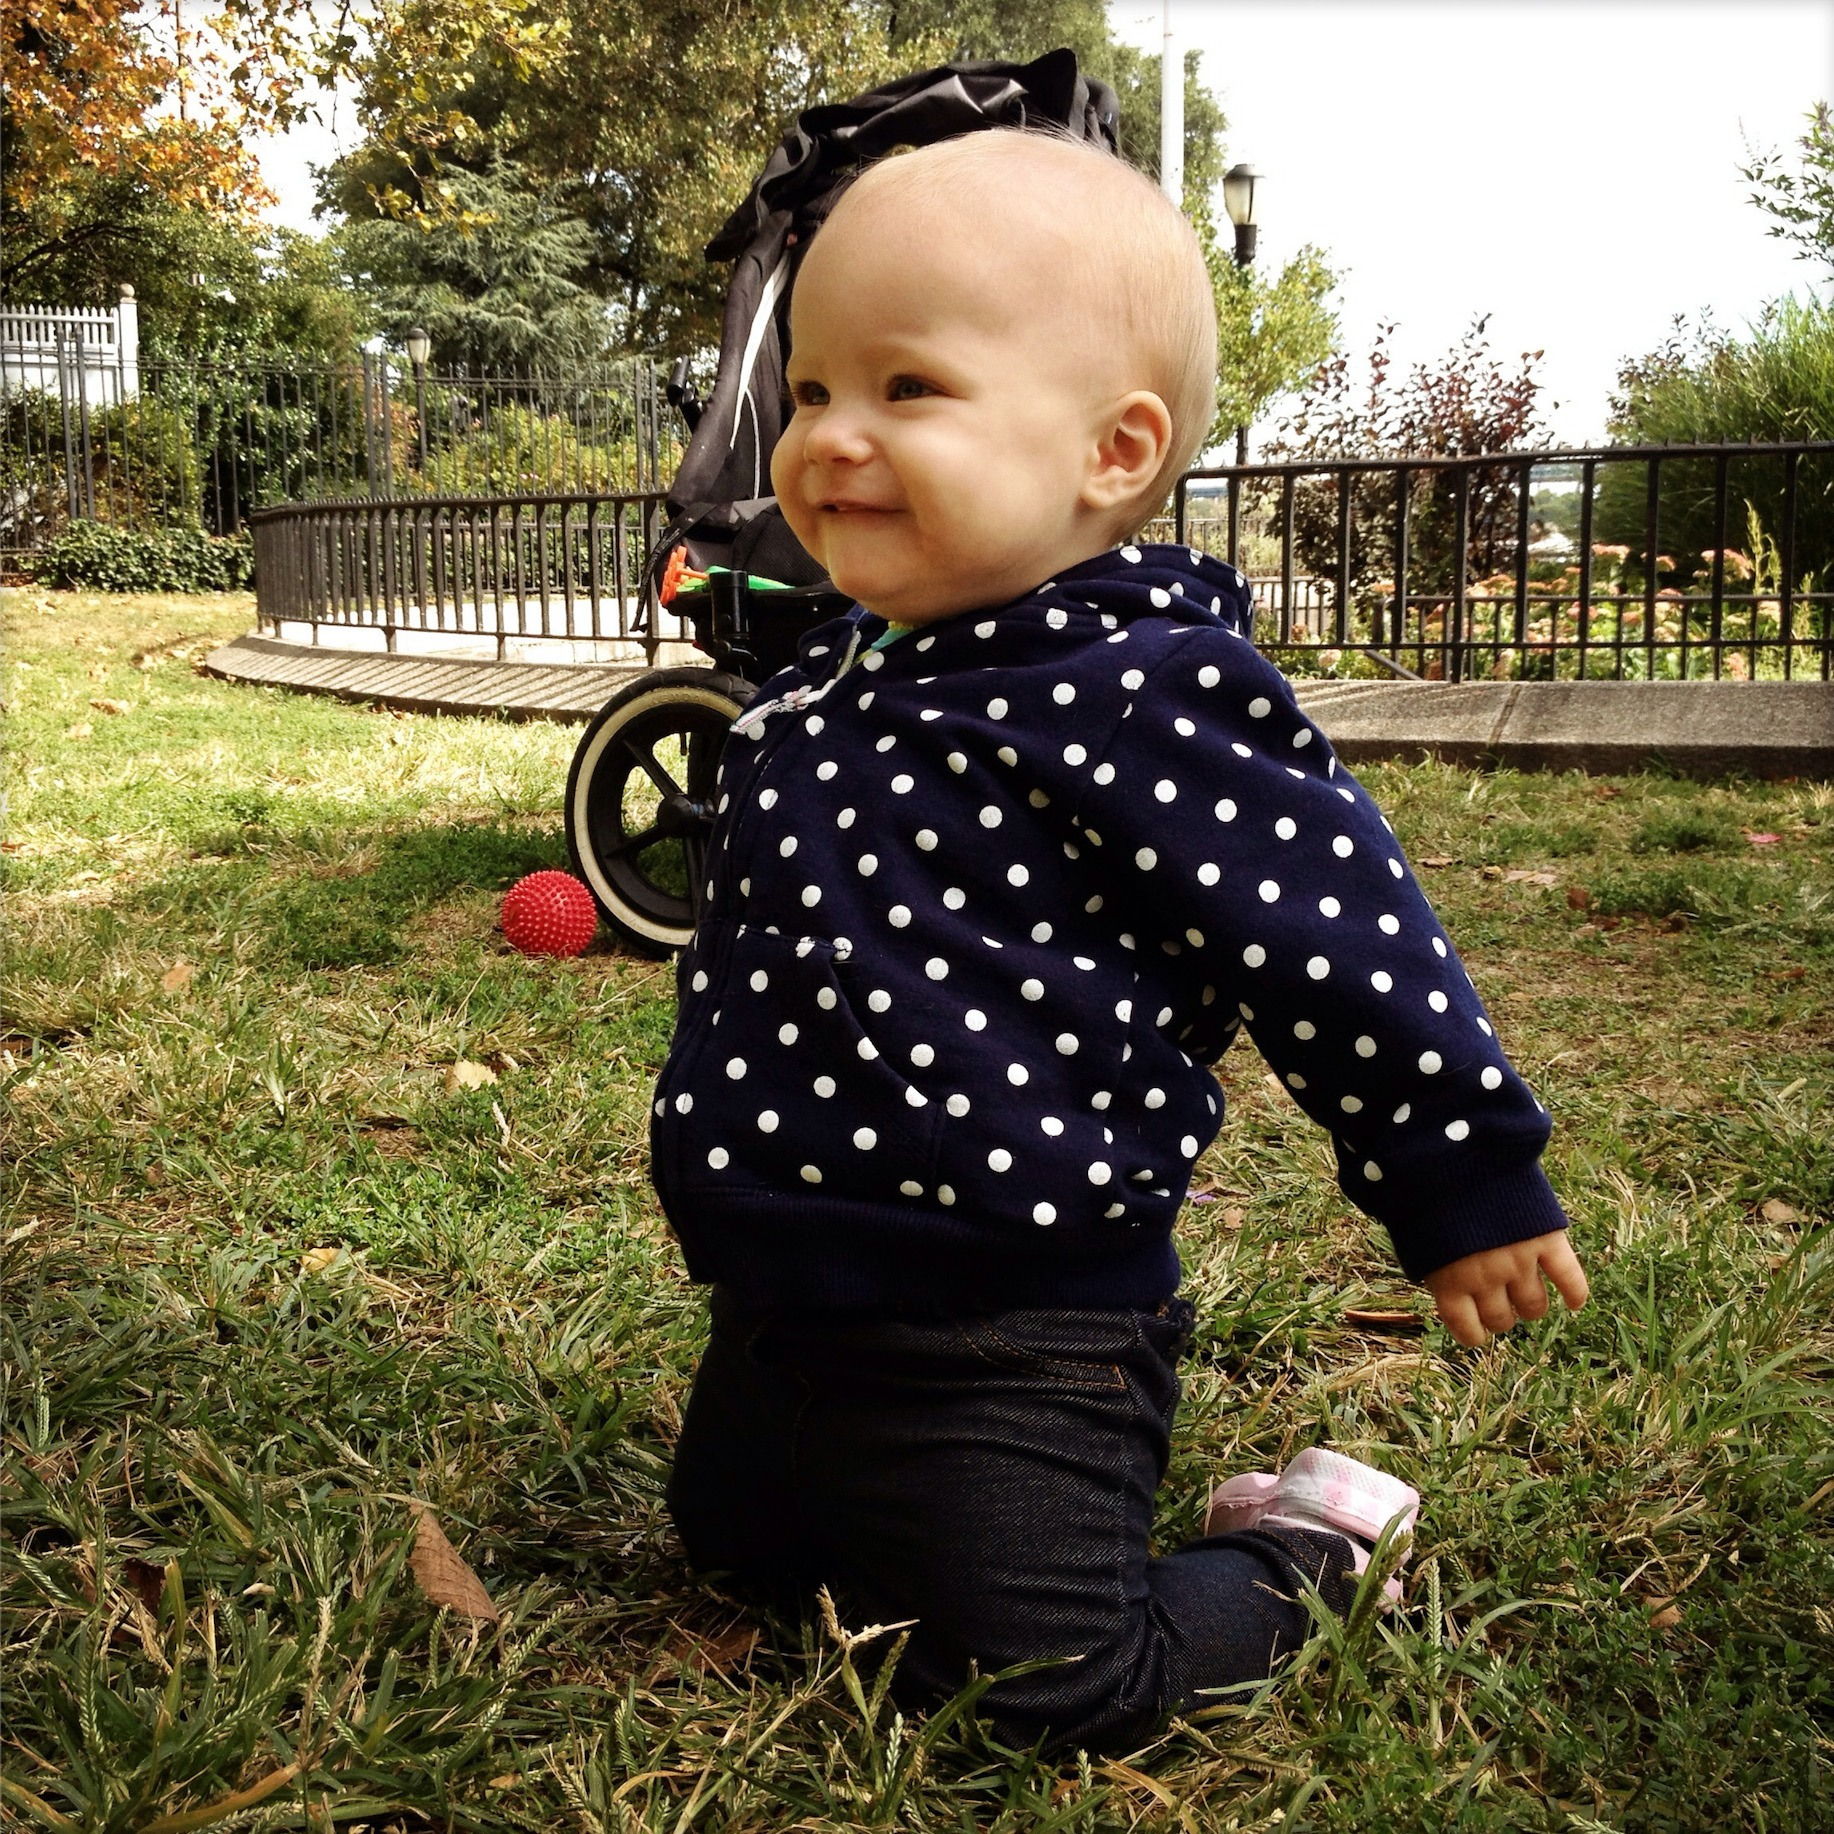
\includegraphics[width=0.2\linewidth]{color-samples/9768152396_c7be0b47bd_o}}
\raisebox{-0.5\height}{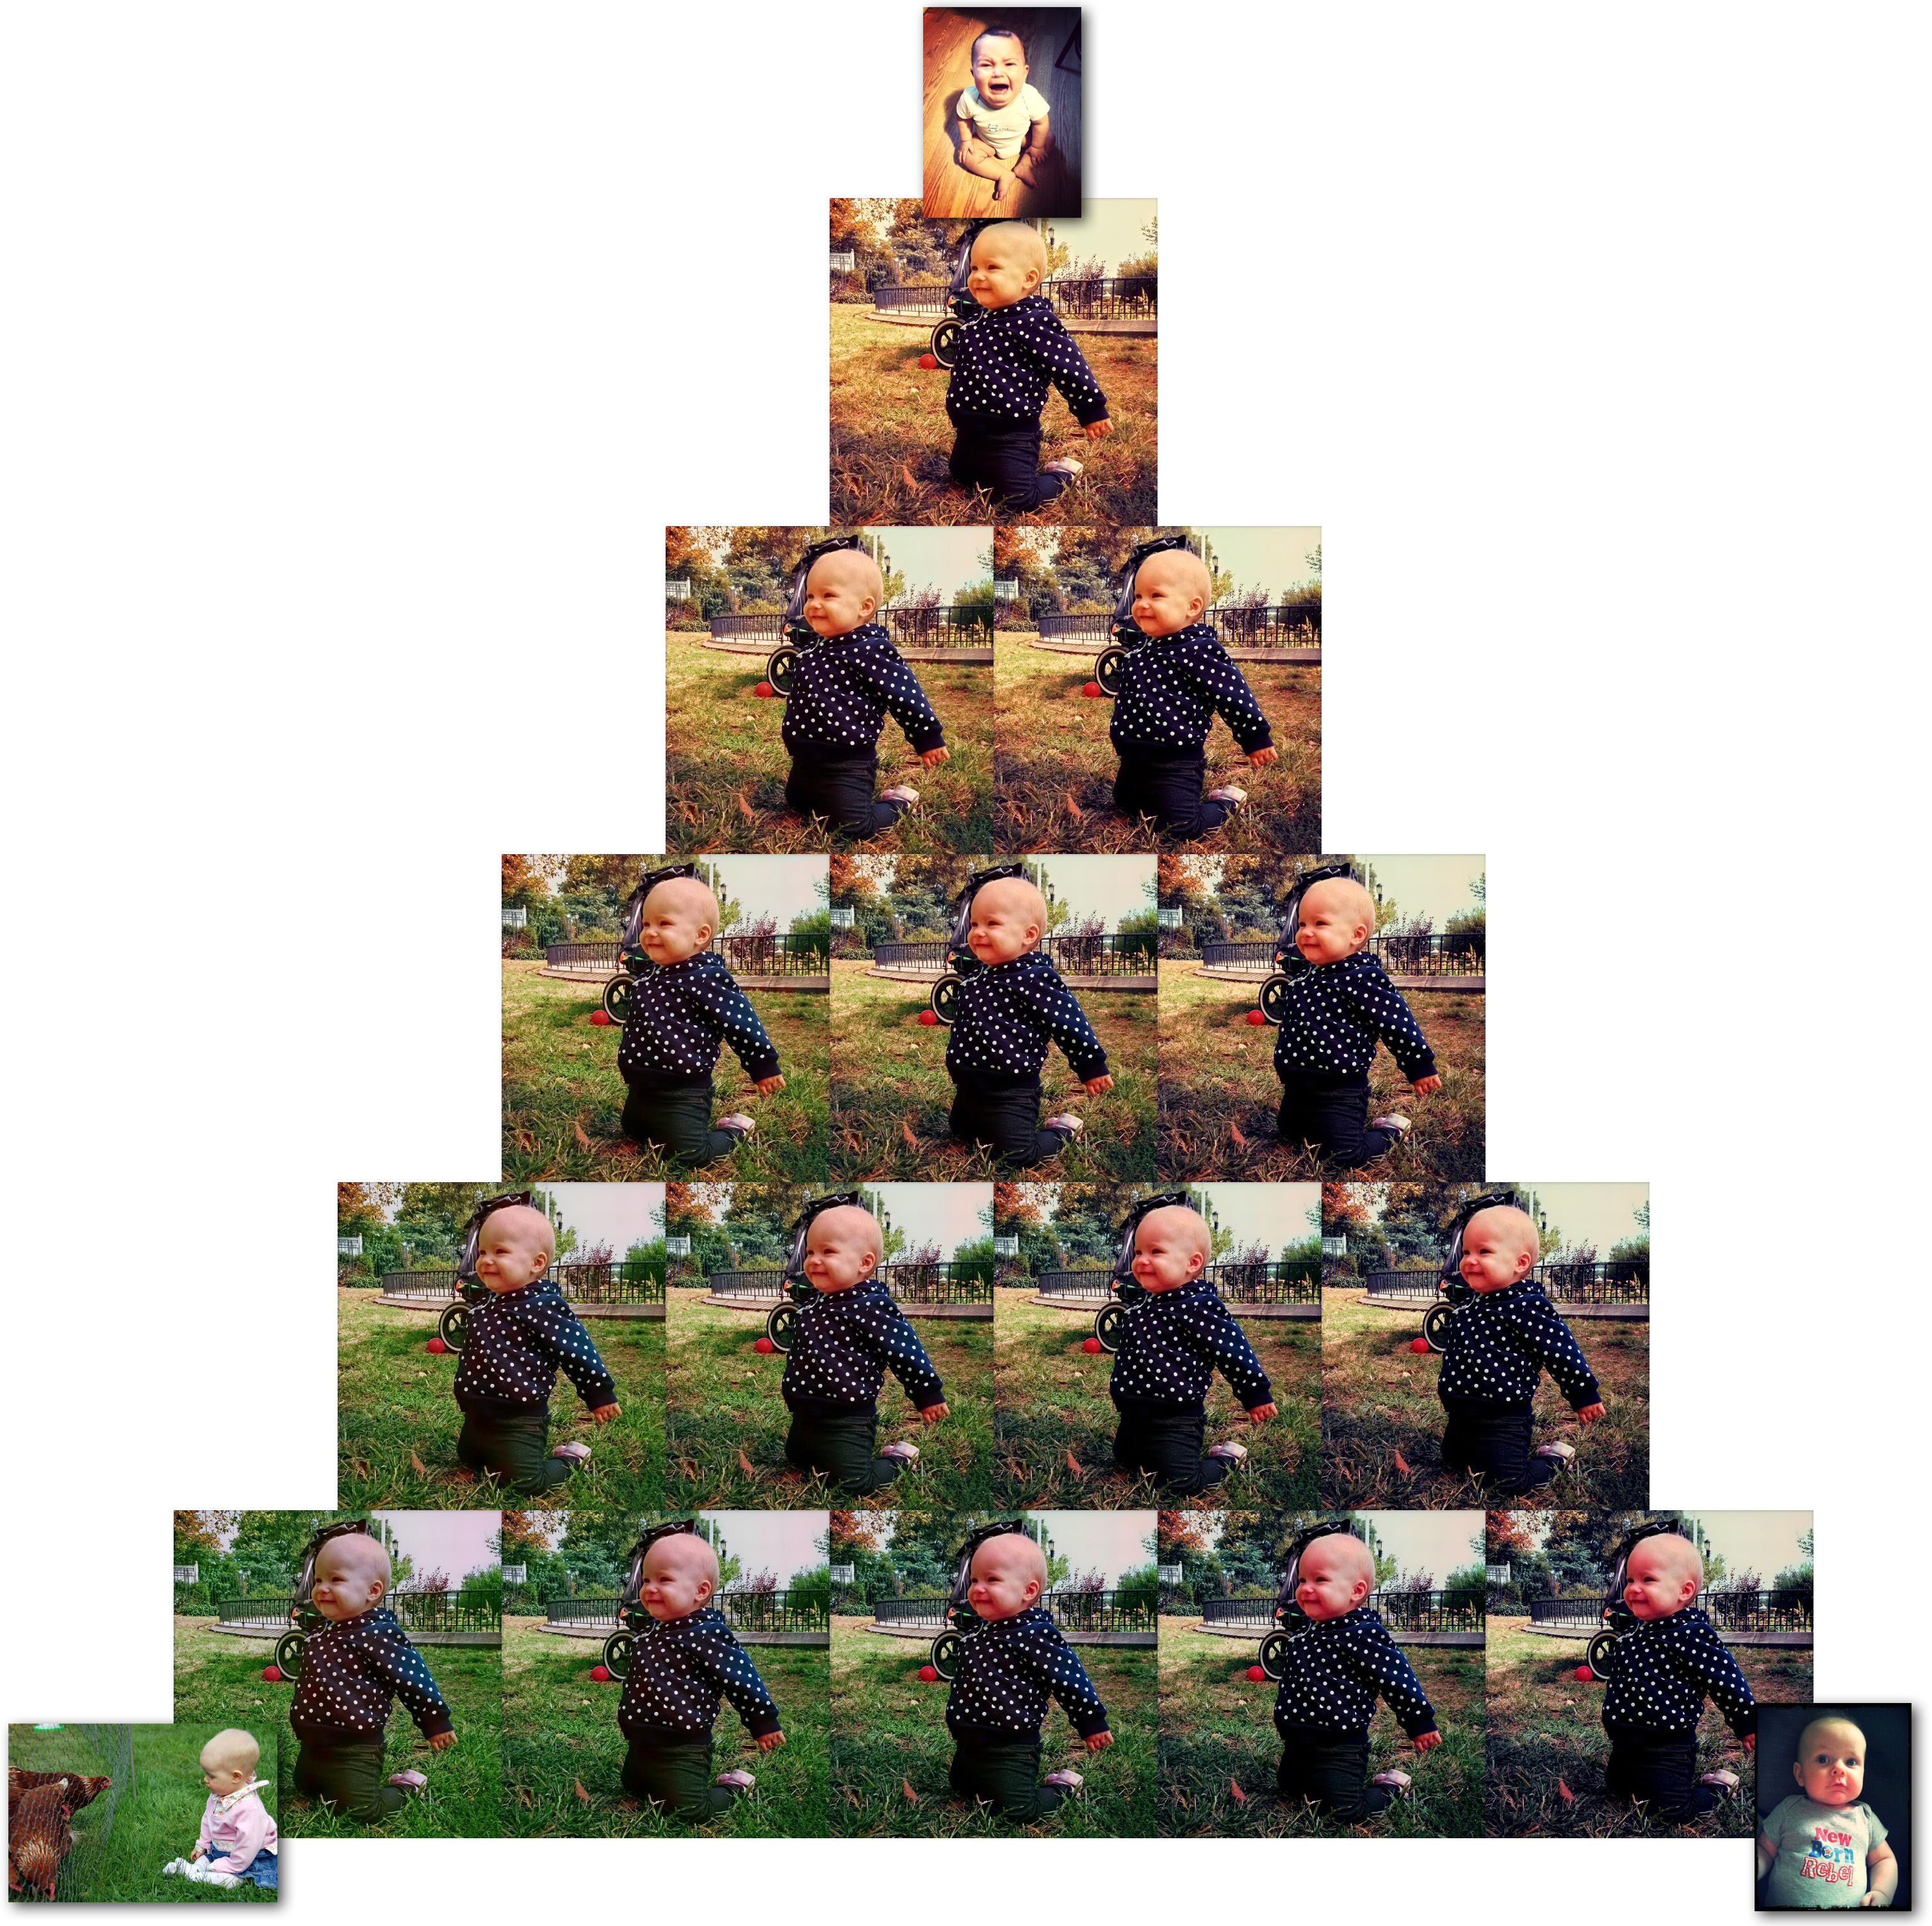
\includegraphics[width=0.65\linewidth]{color2/Proj_H_ok}}\\
\raisebox{-0.5\height}{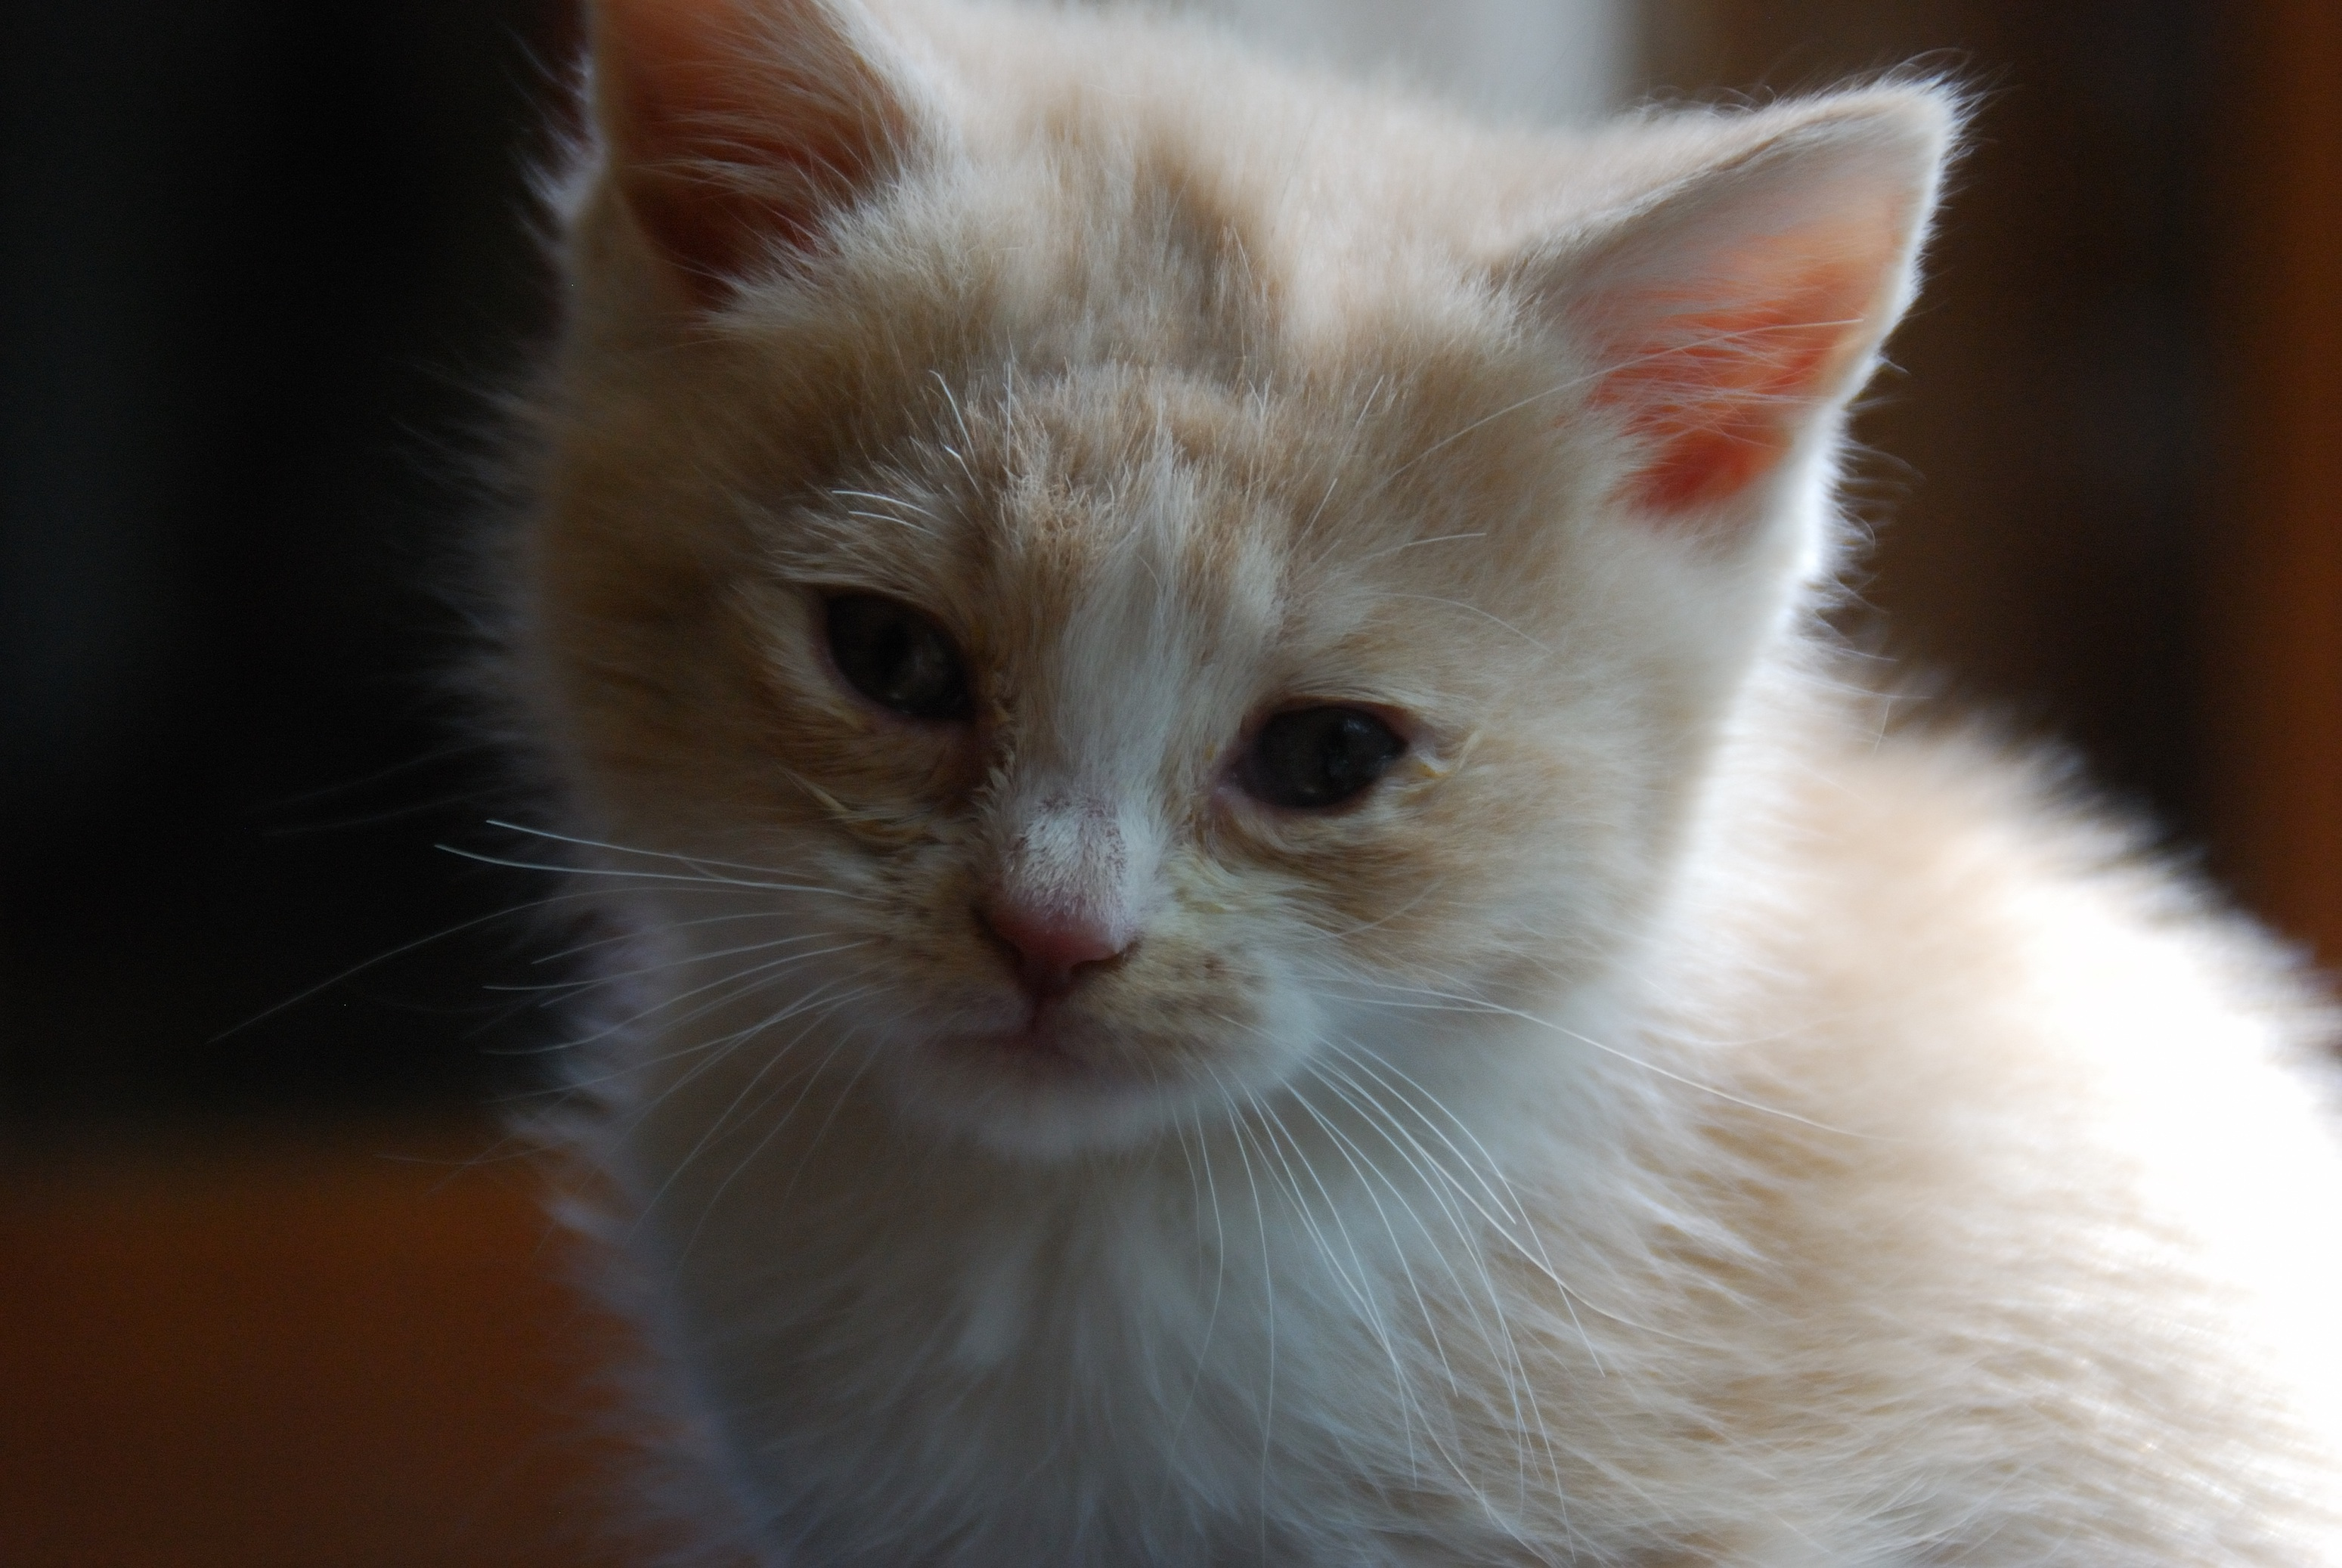
\includegraphics[width=0.2\linewidth]{color-samples/3629553810_f27623de46_o}}
\raisebox{-0.5\height}{\includegraphics[width=0.65\linewidth]{color2/ProjF_ok}}
\end{center}
\caption{Color manipulation by transferring the colors of $|I|=3$ photographs $\{X_i\}_{i \in I}$ (shown at the vertices of the triangle, right) to the initial photograph $\iterInit{X}$ (left) to obtain $X^\star$ which varies in the triangle as a function of the convex weights $\la \in \La_I$. Additional results can be seen in supplemental material.}
\label{fig:colortransfer}
\end{figure*}

%%
\paragraph{Examples.}


\begin{figure}[!t]
\begin{center} 
\includegraphics[width=0.3\linewidth]{color/clockmontague-1} \hspace{1mm}
\includegraphics[width=0.3\linewidth]{color/clockmontague-2}  \hspace{1mm}
\includegraphics[width=0.3\linewidth]{color/clockmontague-3} 
\\
Original images $(X^{(i)})_{i \in I}$.\\ 
\includegraphics[width=0.3\linewidth]{color/Bary_Reg_clockmontague-1} \hspace{1mm}
\includegraphics[width=0.3\linewidth]{color/Bary_Reg_clockmontague-2}  \hspace{1mm}
\includegraphics[width=0.3\linewidth]{color/Bary_Reg_clockmontague-3} 
\\
Harmonized images $\{ X^{(i,\star)} \}_{i \in I}$. 
\end{center}
\vspace{-0.2cm}
\caption{Color harmonization of an image sequence, using $\la_i=1/|I|$ to compute the iso-barycenter (here $|I|=3$). }
\label{fig:colorharmonization}
\end{figure}


Figure~\ref{fig:colorharmonization} shows an example of harmonization, where the color palette is defined as the iso-barycenter of three input color palettes. In Figure~\ref{fig:colortransfer}, the image $\iterInit{X}$ to be modified is not contained in the set of input pictures $\{X^{(i)}\}_{i\in I}$. This allows for the user to navigate over the simplex of color palettes to select the desired one. Table~\ref{tab:weights} provides the corresponding weights for Figure~\ref{fig:colortransfer}.
% Nico: a simplex is necessarily convex, right?


\begin{table}
\caption{Coordinates $w$ used to define the weights $\lambda = w/(\sum_i w_i)$  for the color transfer in Figure~\ref{fig:colortransfer}.}
\label{tab:weights}
\begin{center}
\begin{tabular}{cccccccccc} % |c|c|c|c|c|c|c|c|c|c|
   %\hline
  \multicolumn{4}{c}{  } & \multicolumn{2}{c}{ $\sf (0,0,1)$ } \\
   %\hline
   \multicolumn{3}{c}{  } & \multicolumn{2}{c}{ $\sf (1,0,3)$ } & \multicolumn{2}{c}{ $\sf (0,1,3)$ } \\
   %\hline
   \multicolumn{2}{c}{  } & \multicolumn{2}{c}{ $\sf (1,0,1)$ } & \multicolumn{2}{c}{ $\sf (1,1,2)$ } & \multicolumn{2}{c}{ $\sf (0,1,1)$ } \\
   %\hline
   {\color{white} $\sf (0,$} & \multicolumn{2}{c}{ $\sf (3,0,1)$ } & \multicolumn{2}{c}{ $\sf (2,1,1)$ } & \multicolumn{2}{c}{ $\sf (1,2,1)$ } & \multicolumn{2}{c}{ $\sf (0,3,1) $}  \\
   %\hline
   \multicolumn{2}{c}{ $\sf (1,0,0)$ }  & \multicolumn{2}{c}{ $\sf (3,1,0)$ } & \multicolumn{2}{c}{ $\sf (1,1,0)$ } & \multicolumn{2}{c}{ $\sf (1,3,0)$ } & \multicolumn{2}{c}{ $\sf (0,1,0)$ }  
   %\hline
\end{tabular}
\end{center}
\end{table}


% \begin{figure*}[!t]
% \setlength{\tabcolsep}{10pt}
  % \setlength{\fboxsep}{0pt}
  
% \begin{center} 
% \begin{tabular}{c c}
% \includegraphics[width=0.16\linewidth]{color/4625786629_1808574482_b} \hfill
% \includegraphics[width=0.16\linewidth]{color/8245632244_78ca92ed42_h} \hfill 
% \includegraphics[width=0.16\linewidth]{color/8581254643_8ead330c4c_h} 
% &
% \\

% (a)  & (b)   \\

% \includegraphics[width=0.16\linewidth]{color/Bary_Reg_4625786629_1808574482_b} \hfill
% \includegraphics[width=0.16\linewidth]{color/Bary_Reg_8245632244_78ca92ed42_h} \hfill 
% \includegraphics[width=0.16\linewidth]{color/Bary_Reg_8581254643_8ead330c4c_h} 

% &
% \\

% (c) & (d) \\

% \includegraphics[width=0.48\linewidth]{color/Proj_4625786629_1808574482_b} &
% \includegraphics[width=0.48\linewidth]{color/Proj_girls} \\

% (e) & (f) \\
% \end{tabular}
% \end{center}
% \caption{}
% \label{fig:colortransfer2}
% \end{figure*}